% Customizable fields and text areas start with % >> below.
% Lines starting with the comment character (%) are normally removed before release outside the collaboration, but not those comments ending lines

% svn info. These are modified by svn at checkout time.
% The last version of these macros found before the maketitle will be the one on the front page,
% so only the main file is tracked.
% Do not edit by hand!
\RCS$Revision: 340136 $
\RCS$HeadURL: svn+ssh://nckw@svn.cern.ch/reps/tdr2/papers/EXO-12-055/trunk/EXO-12-055.tex $
\RCS$Id: EXO-12-055.tex 340136 2016-04-26 16:32:55Z nckw $
%%%%%%%%%%%%% local definitions %%%%%%%%%%%%%%%%%%%%%
% This allows for switching between one column and two column (cms@external) layouts
% The widths should  be modified for your particular figures. You'll need additional copies if you have more than one standard figure size.
\newlength\cmsFigWidth
\newcommand{\Zmm}{\ensuremath{\textrm{Z}\to\mu^+\mu^-}}
\newcommand{\Zvv}{\ensuremath{\textrm{Z}\to\nu\nu}}
\newcommand{\Wlv}{\ensuremath{\textrm{W}\to l\nu}}
\newcommand{\Zmmjets}{\ensuremath{\textrm{Z}(\mu\mu)+\textrm{jets}}}
\newcommand{\Vjets}{\ensuremath{\textrm{V}+\textrm{jets}}}
\newcommand{\Zjets}{\ensuremath{\textrm{Z}+\textrm{jets}}}
\newcommand{\Zlljets}{\ensuremath{\textrm{Z}(ll)+\textrm{jets}}}
\newcommand{\Zvvjets}{\ensuremath{\textrm{Z}(\nu\nu)+\textrm{jets}}}
\newcommand{\Wlvjets}{\ensuremath{\textrm{W}(l\nu)+\textrm{jets}}}
\newcommand{\Wmvjets}{\ensuremath{\textrm{W}(\mu\nu)+\textrm{jets}}}
\newcommand{\phojets}{\ensuremath{\gamma+\textrm{jets}}}
\newcommand{\brhiggs}{\ensuremath{0.62}}
\newcommand{\higgsbr}{\ensuremath{0.62}}
\newcommand{\higgsbrobs}{\ensuremath{0.53}}
\newcommand{\pt}{\ensuremath{p_{\mathrm{T}}}}
\newcommand\numberthis{\addtocounter{equation}{1}\tag{\theequation}}

\ifthenelse{\boolean{cms@external}}{\setlength\cmsFigWidth{0.85\columnwidth}}{\setlength\cmsFigWidth{0.4\textwidth}}
\ifthenelse{\boolean{cms@external}}{\providecommand{\cmsLeft}{top\xspace}}{\providecommand{\cmsLeft}{left\xspace}}
\ifthenelse{\boolean{cms@external}}{\providecommand{\cmsRight}{bottom\xspace}}{\providecommand{\cmsRight}{right\xspace}}
%%%%%%%%%%%%%%%  Title page %%%%%%%%%%%%%%%%%%%%%%%%
\cmsNoteHeader{EXO-12-055} % This is over-written in the CMS environment: useful as preprint no. for export versions
% >> Title: please make sure that the non-TeX equivalent is in PDFTitle below
\title{Search for dark matter with CMS at $\sqrt{s}=8$ TeV in events with missing transverse energy and jets including those from hadronically decaying vector bosons.}

% >> Authors
%Author is always "The CMS Collaboration" for PAS and papers, so author, etc, below will be ignored in those cases
%For multiple affiliations, create an address entry for the combination
%To mark authors as primary, use the \author* form
\address[neu]{Northeastern University}
\address[fnal]{Fermilab}
\address[cern]{CERN}
\author[cern]{The CMS Collaboration}

% >> Date
% The date is in yyyy/mm/dd format. Today has been
% redefined to match, but if the date needs to be fixed, please write it in this fashion.
% For papers and PAS, \today is taken as the date the head file (this one) was last modified according to svn: see the RCS Id string above.
% For the final version it is best to "touch" the head file to make sure it has the latest date.
\date{\today}

% >> Abstract
% Abstract processing:
% 1. **DO NOT use \include or \input** to include the abstract: our abstract extractor will not search through other files than this one.
% 2. **DO NOT use %**                  to comment out sections of the abstract: the extractor will still grab those lines (and they won't be comments any longer!).
% 3. For PASs: **DO NOT use tex macros**         in the abstract: CDS MathJax processor used on the abstract doesn't understand them _and_ will only look within $$. The abstracts for papers are hand formatted so macros are okay.
\abstract{
A search is presented for an excess of events with large missing transverse energy in association with a highly energetic jet in a data sample of proton-proton 
interactions at a centre-of-mass energy of 8 TeV. The data correspond to an integrated luminosity of 19.7 $\textrm{fb}^{-1}$ collected by the CMS detector at the LHC. 
The results are interpreted under a set of simplified models describing the production of dark matter via a scalar,
pseudoscalar, vector, or axial vector mediator. 
Additional sensitivity is achieved by tagging events consistent with the jet originating from a boosted hadronically decaying vector boson. 
}

% >> PDF Metadata
% Do not comment out the following hypersetup lines (metadata). They will disappear in NODRAFT mode and are needed by CDS.
% Also: make sure that the values of the metadata items are sensible and are in plain text:
% (1) no TeX! -- for \sqrt{s} use sqrt(s) -- this will show with extra quote marks in the draft version but is okay).
% (2) no %.
% (3) No curly braces {}.
\hypersetup{%
pdfauthor={CMS Collaboration},%
pdftitle={Search for dark matter with CMS at $\sqrt{s}=8$ TeV in events with missing transverse energy and jets including those from hadronically decaying vector bosons.},%
pdfsubject={CMS},%
pdfkeywords={CMS, physics, software, computing}}

\maketitle %maketitle comes after all the front information has been supplied
% >> Text
%%%%%%%%%%%%%%%%%%%%%%%%%%%%%%%%%%%%%%%%%%%%%%
%%%%%%%%%%%%%%%%%%%%%%%%%%%%%%%%%%%%%%%%%%%%%%
\section{Introduction}
%%%%%%%%%%%%%%%%%%%%%%%%%%%%%%%%%%%%%%%%%%%%%%
%%%%%%%%%%%%%%%%%%%%%%%%%%%%%%%%%%%%%%%%%%%%%%
This paper describes a search for dark matter (DM) in events containing an
energetic jet and an imbalance of transverse energy (\ETm) in 
proton-proton (pp) collisions at a centre-of-mass energy of 8 TeV. 
The data correspond to an integrated luminosity of  19.7\fbinv collected 
using the Compact Muon Solenoid (CMS) detector at the CERN Large Hadron Collider (LHC).

The existence of DM is one of the most compelling sources of evidence
for physics beyond the standard model (SM) of particle physics, with a number of astrophysical
observations suggesting an abundance of a nonbaryonic form of matter in the
universe. In many theories which extend the SM, the production of DM particles
is possible at the LHC. Monojet searches~\cite{monojet1,monojet2,ATLAS:2012ky,Aad:2011xw,Chatrchyan:2012me,Khachatryan:2016reg} provide  
sensitivity to a wide range of models for  DM production at the LHC, while mono-V 
(where V=W or Z boson) searches~\cite{monolep,Aad:2014vka,Aad:2013oja,ATLAS:2014wra} target models with 
associated production of DM with SM vector bosons. While the mono-V searches target more specific models, 
they benefit from smaller contributions from SM backgrounds. 
%which can be enhanced in
%theories with non-universal DM couplings~\cite{IVDM}.  
The interpretation of
results from these and other DM searches at the LHC have generally utilized
effective field theories (EFT) that assume heavy mediators and DM production via
contact interactions~\cite{Fox:2011pm}.  The results of this analysis are
interpreted in the context of a spin-0 or spin-1 mediator decaying to DM pairs
under a set of simplified DM
models~\cite{simplified1,Buchmueller:2013dya,Buchmueller:2014yoa},  which span a broad range of mediator and DM 
particle properties~\cite{Abercrombie:2015wmb}. This allows for a comparison in sensitivity with respect to
direct detection(DD) experiments while retaining validity as a description of DM
production across the entire kinematic region accessible at the LHC. 

This search is the first at CMS to target the hadronic decay modes of the vector
bosons in the mono-V channels. The 
mono-V search uses recently developed techniques designed to exploit information 
available in the jet's substructure when the V-boson is 
highly boosted and uses a multivariate V-tagging technique to
identify the individual jets from moderately boosted V-bosons.  
The events are categorized according to the nature of the jets in the
event. The signal extraction is performed by considering the $\ETm$
distribution in each event category, and using additional data control regions 
to constrain the dominant backgrounds yielding improvements of roughly 60\% and 40\% respectively 
in exclusion limits in comparison with the previous CMS monojet analysis~\cite{monojet1}.

This paper is structured as follows:Section 2 provides a description of the 
CMS detector; Section 3 outlines the DM models
explored as signal hypotheses; Section 4 provides a description of the
physics object reconstruction, event selection and categorization used in
the search; Section 5 describes the background modelling used for the signal
extraction; Section 6 presents the results and interpretations in  
the context of simplified models for DM production.

%===============================================================================
\section{CMS detector}

The CMS detector, described in detail in Ref.~\cite{CMSdetector}, is a
multi-purpose apparatus designed to study high-transverse momentum($\pt$) physics processes in
proton-proton and heavy-ion collisions.  A superconducting solenoid occupies its
central region, providing a magnetic field of 3.8\unit{T} parallel to the beam
direction. Charged-particle trajectories are measured by the silicon pixel and
strip trackers, which cover a pseudorapidity region of $\abs{\eta} < 2.5$. A
lead tungstate (PbWO$_4$) crystal electromagnetic calorimeter (ECAL) and a
brass and scintillator hadron calorimeter (HCAL) surround the tracking volume and
cover $\abs{\eta} < 3$. The steel/quartz-fiber Cherenkov hadron forward (HF)
calorimeter extends the coverage to $\abs{\eta} < 5$.  The muon system consists
of gas-ionization detectors embedded in the steel flux-return yoke outside the
solenoid, and covers $\abs{\eta} < 2.4$. The first level of the CMS trigger
system, composed of custom hardware processors, is designed to select the most
interesting events in less than 4\mus, using information from the calorimeters
and muon detectors. The high-level trigger processor farm then further reduces
the event rate to a few hundred Hz.  

\section{Signal hypotheses} 
The signal hypotheses targeted in this search are provided under a set of simplified
mediator models~\cite{simplified1,Buchmueller:2013dya,Buchmueller:2014yoa}. 
These models assume an additional particle, a fermionic dark
matter candidate, and an additional interaction that forces the production of DM.  
It is assumed that this additional interaction is mediated by a
generic spin-0 or spin-1 particle.  The interactions are characterised by four
distinct Lagrangians, written for a Dirac-fermion DM particle $\chi$
with mass $m_{\mathrm{DM}}$ and mediator~($S$, $P$, $Z'$, $Z''$) with mass $m_{\mathrm{MED}}$ as, 

\begin{align} \label{eq:LS} \mathcal{L}_{\mathrm{scalar}}&\supset\,
-\,\frac{1}{2}m_{\rm MED}^2 S^2 - g_{\rm DM}  S \, \bar{\chi}\chi - \sum_{q=b,t}
g_{\rm SM}^q S \, \bar{q}q  - m_{\rm DM} \bar{\chi}\chi \,, \\ \label{eq:LP}
\mathcal{L}_{\rm{pseudoscalar}}&\supset\, -\,\frac{1}{2}m_{\rm MED}^2 P^2 - i
g_{\rm DM}  P \, \bar{\chi} \gamma^5\chi -\sum_{q=b,t}  i g_{\rm SM}^q  P \, \bar{q}
\gamma^5q  - m_{\rm DM} \bar{\chi}\chi\,, \\ \label{eq:LV}
\mathcal{L}_{\mathrm{vector}}&\supset \, \frac{1}{2}m_{\rm MED}^2 Z'_{\mu}
Z'^{\mu} - g_{\rm DM}Z'_{\mu} \bar{\chi}\gamma^{\mu}\chi -\sum_q g_{\rm SM}^q
Z'_{\mu} \bar{q}\gamma^{\mu}q - m_{\rm DM} \bar{\chi}\chi\,, \\ \label{eq:LA}
\mathcal{L}_{\rm{axial-vector}}&\supset\,  \frac{1}{2}m_{\rm MED}^2 Z''_{\mu}
Z''^{\mu} - g_{\rm DM} Z''_{\mu} \bar{\chi}\gamma^{\mu}\gamma^5\chi -\sum_q
g_{\rm SM}^q Z''_{\mu} \bar{q}\gamma^{\mu}\gamma^5q - m_{\rm DM} \bar{\chi}\chi,\,
\end{align}

assuming pure scalar, pseudoscalar, vector, and axial vector mediated
interactions denoted by $S,~P,~Z'$ and $Z''$ mediators, respectively.  The
terms $g_{\mathrm{DM}}$ and $g_{\mathrm{SM}}$ denote the couplings
of the mediator to the DM particle and to SM particles, respectively~\cite{Harris:2014hga}.  
In all models considered, the couplings are assumed to be unity ($g_{\mathrm{SM}}=g_{\mathrm{DM}}=1$). 
For the scalar and pseudoscalar models, this denotes a Yukawa coupling to SM particles.
The choice of the split in terms of axial vector and vector mediators in the Lagrangian is to
parallel the existing separation with direct detection, into spin-dependent and
spin-independent interactions. Here, spin-independent can refer to either vector
or scalar mediated interactions, between which DD makes no
distinction, while spin-dependent interactions refer to axial vector mediated
processes.
 
Pseudoscalar DM-nucleon interaction cross sections are suppressed at non-relativistic DM 
velocities which limits the sensitivity from direct detection experiments~\cite{Haisch:2012kf,LopezHonorez:2012kv}.  
An extension to the scalar and pseudoscalar can
be performed by allowing the scalar and pseudoscalar interactions to undergo
electroweak symmetry breaking in an analogous way to the Higgs
mechanism~\cite{Khoze:2015sra,Hambye:2013sna,Khoze:2014xha,Khoze:2014woa,Altmannshofer:2014vra,Carone:2013wla,Heikinheimo:2013fta}.  
In collider experiments, the production of Dark Matter in spin-0 mediated
interactions is predominantly through gluon-fusion via a top-quark loop 
(Fig. ~\ref{fig:monoXfeyn}(a)).  When couplings of the mediator to vector bosons are 
present, mono-V 
signatures are produced through a radiative process (Fig.~\ref{fig:monoXfeyn}(b)). 
The scenario in which couplings between the mediator and vector bosons are not considered, is 
denoted herein as $fermionic$. 
For the spin-1 signatures, DM is produced in
an analogous way to Z boson production (Fig.~\ref{fig:monoXfeyn}(c,d)). The
mono-V or monojet signatures follow from the presence of a V-boson or
jet in the initial state. 
For the fermionic models, the width is determined under the minimum width constraint 
requiring that only quarks and DM particles couple to the mediator. For the case in 
which couplings between the mediator and V-bosons are allowed, the width is modified to 
account for the additional contributions which these couplings allow~\cite{Harris:2014hga}.

In order to model the expected contribution from these signals, simulated 
events are generated using MCFM~6.8\cite{mcfm} for the monojet final state, and
JHUGen~5.2.5~\cite{Anderson:2013afp} for the V-boson signature.
All signal models are generated at leading order, using  
PYTHIA~6.4.26~\cite{Sjostrand:2006za} for parton showers and hadronization, and Geant4~\cite{geant4} for simulation of the CMS detector response.  
For the monojet signal, the generation is performed using the mediator mass for both the generation and hadronisation scale. 
An alternative choice taking the boson $\pt$ for the hadronisation scale was found to result in differences between  
$30-80$\% in the expected signal yield in the relevant kinematic region for mediator masses above 400\GeV. 
For scalar and pseudoscalar mediated DM production, the finite top quark mass is taken 
into account for both the inclusive and differential cross-section. NNPDF3.0 used to
specify the parton distribution function inputs in the signal generation~\cite{Ball:2014uwa}.

\begin{figure}[htbp] \centering \subfloat[][]{
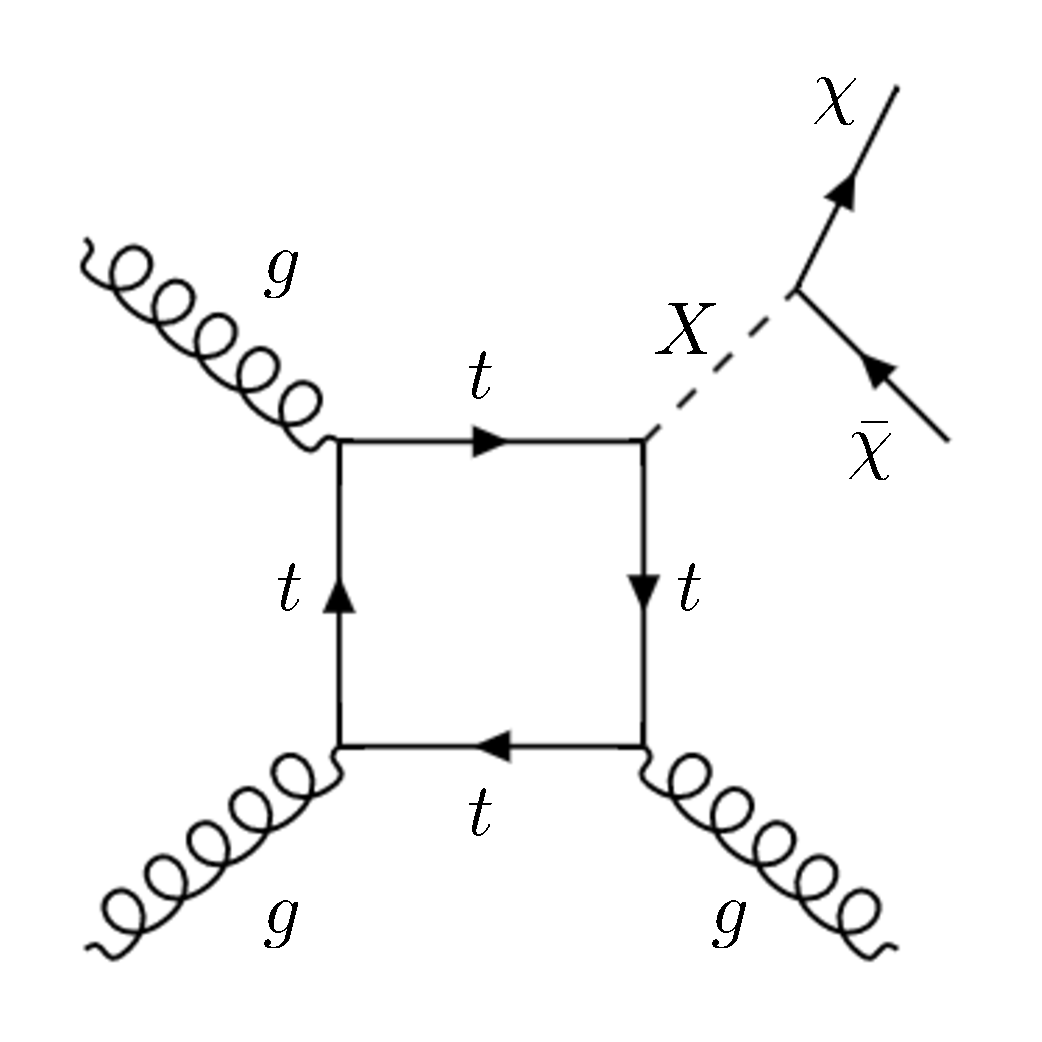
\includegraphics[angle=0,width=0.36\textwidth]{figures/scalarbox.pdf}
\label{fig:monojet0} } \subfloat[][]{
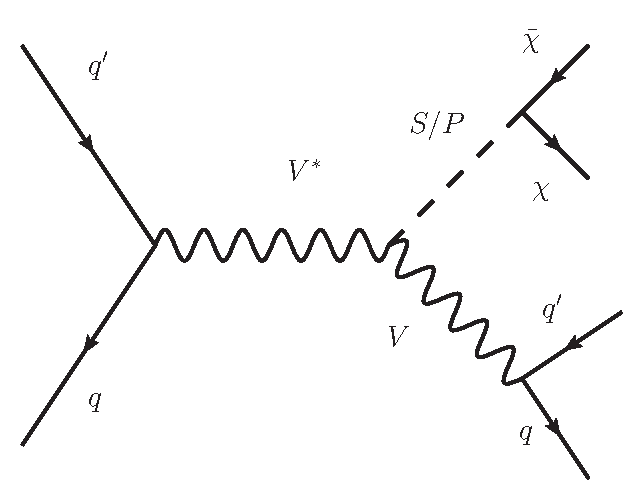
\includegraphics[angle=0,width=0.36\textwidth]{figures/scalarV.pdf}
\label{fig:monoV0} }\\ \subfloat[][]{
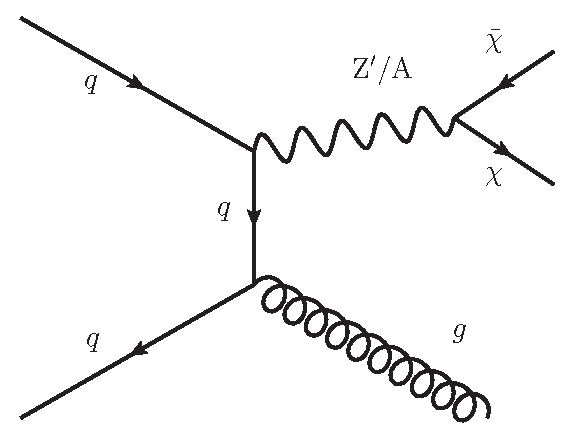
\includegraphics[angle=0,width=0.36\textwidth]{figures/vectorJ.pdf}
\label{fig:monojet1} } \subfloat[][]{
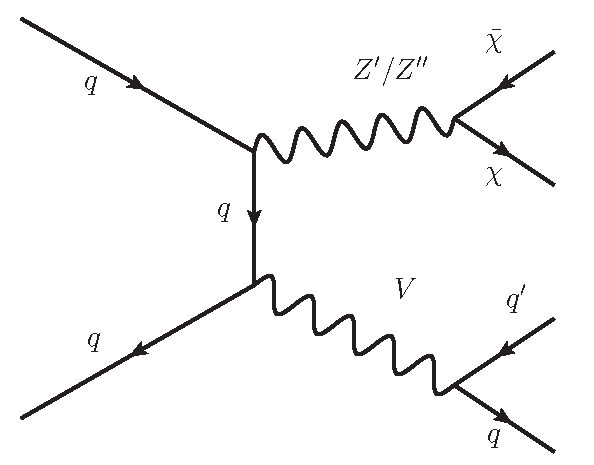
\includegraphics[angle=0,width=0.36\textwidth]{figures/vectorV.pdf}
\label{fig:monojet2} } 
\caption{Diagrams for production of DM via mediator (X) in the cases
  of a scalar/pseudoscalar mediator providing (a) monojet and (b) mono-V signatures. 
  Diagrams for production of DM via a vector/axial vector mediator providing 
  (c) monojet and (d) mono-V signatures. \label{fig:monoXfeyn}} \end{figure}


\section{Event selection and categorization}\label{sec:selection}

Candidate signal events are selected on the basis of large values of
missing transverse energy (\ETm) and
one or more high-\pt jets~\cite{CMSdetector}. 

The data used for this analysis are collected using two \ETm triggers 
The first requires an \ETm of
greater than 120 \GeV, calculated only using information from the calorimeters,
while the second requires an \ETm greater than 95~\GeV or 105~\GeV, depending on
the data-taking period, together with at least one jet of \pt$>80$ \GeV and
$|\eta|<2.6$. The $\ETm$ is  calculated using the particle flow (PF) reconstruction
algorithm~\cite{CMS-PAS-PFT-09-001} which optimally combines information from various components 
of the CMS detector to reconstruct and identify individual particles. 
The lowest threshold on \ETm for event selection is set at 200 \GeV 
in order to ensure Done a trigger efficiency greater than 99\% for selected events. 

Jets are reconstructed from the clustering of PF objects using both 
the anti-$k_{\textrm{T}}$ algorithm~\cite{Cacciari:2008gp} with 0.5 (ak5 jet) as
the distance parameter, and the Cambridge/Aachen algorithm~\cite{cajets} with
0.8 distance parameter (ca8). The leading jet is further required to pass standard 
CMS identification criteria~\cite{jec}. The jets
are corrected for contamination from additional, synchornous
interactions (pileup, PU) on the basis of the observed event energy density~\cite{jec}. 
Further corrections are then applied to calibrate the absolute scale of the jet energy~\cite{jec}.

The \ETm is calculated as the magnitude of the negative vector sum of the
transverse momenta of all final state particles, which are reconstructed using PF.  
Events with a large mis-reconstructed \ETm are removed by applying a quality filter on the tracker, 
ECAL, HCAL and muon detector data.

The angle between the \ETm direction and the leading jet in the plane transverse to the
beam line, $\Delta\phi$, is required to be larger than 2 radians to reduce the
contribution from QCD multijet events. Finally, events are vetoed if they
contain at least one well-identified electron, photon or muon with
$\pt>10$~\gev, or a $\tau$ lepton with
$\pt>15$~\gev~\cite{Khachatryan:2015iwa,Khachatryan:2015hwa,Khachatryan:2015dfa,Chatrchyan:2013sba}. The
electron, $\tau$ lepton and photon vetoes require that the  
identified object be isolated using standard PF isolation algorithms~\cite{Beaudette:2014cea}.

Selected events are classified based on the
topology of the jets in order to distinguish initial or final state radiation 
from hadronic V-boson decays which can be either highly boosted or resolved into 2 jets. 
This results in three orthogonal categories of events which are referred to as monojet, V-boosted,  
and V-resolved. The V-boosted and V-resolved categories are collectively referred to as V-tag. 

To compute the SM background expectation, simulated samples are
produced at leading order for the Z+jets, W+jets, $\mathrm{t\bar{t}}$,
single top quark, and QCD multijet processes using
Madgraph~5.1.3~\cite{amcatnlo} interfaced CT10 pdf set~\cite{Gao:2013xoa},
and  with PYTHIA~6.4.26a for
hadronization and fragmentation, where jets from the matrix element calculations are matched
to the parton shower following the MLM matching
prescription~\cite{Mangano:2006rw}.  Additionally a single top quark background
sample, produced at next-to-leading order with {\sc Powheg~1.0} ~\cite{Nason:2004rx,Frixione:2007vw,powheg,Alioli:2010xd,Alioli:2009je}, and a set of diboson samples,
produced at leading order directly with {\sc Pythia6}; all samples are added using
the CT10 pdfset~\cite{Gao:2013xoa}.  The MC samples are corrected to
account for the distribution of the number of additional pileup 
interactions observed in the 8 TeV dataset. Both signal and background samples are
additionally corrected to account for the mismodelling of hadronic recoil in
simulation following the procedure described in Ref.~\cite{CMS-PAS-JME-12-002}.


%between initial or final state
%radiation of gluons or quarks and jets arising from hadronic vector boson
%decays.  The events are first distinguished by the presence of an single jet
%containing the full quark decays of a vector boson (boosted category),
%subsequently for a resolved vector boson (resolved category), and finally the
%remaining events are collected into the monojet category. 

If the vector boson decays hadronically and has sufficiently large~\pt, both its hadronic decay products are captured by a single
reconstructed ``fat'' jet.  Events in the V-boosted category are
required to have a reconstructed ca8 jet with $\pt>200$ \GeV and  $\ETm>250$
\GeV.  Further selection criteria are applied to improve the vector boson jet purity by
cutting on the ``N-subjettiness'' ratio $\tau_2/\tau_1$ as defined 
in Refs.~\cite{Thaler:2010tr,Thaler:2011gf}, which identifies jets with a two sub-jet
topology, and the pruned jet mass ($m_{\mathrm{prune}}$)~\cite{Ellis:2009me}.
The $\tau_2/\tau_1$ ratio is required to be smaller than 0.5 and $m_{\mathrm{prune}}$ 
is required to be in the range 60-110 \GeV.  
Events which contain additional jets close to the ca8 jet, but no closer than $\Delta R <
0.5$, are selected to include the frequent cases in which initial state
radiation yields additional jets. If an ak5 jet with $\pt>30$~\GeV and $|\eta|<2.5$
is reconstructed, and the opening azimuthal angle between it and the ca8 jet
is smaller than 2 radians, the event is selected, otherwise it is rejected. Events
with more than one ak5 jet with $\pt>30$ \GeV and $|\eta|<2.5$, reconstructed
at $\Delta R> 0.5$ with respect to the ca8 jet are rejected.
Figure~\ref{fig:boostvtagvars} shows the distributions of $\tau_2/\tau_1$ and
$m_{\mathrm{prune}}$, before the application of the jet mass selection, in simulation
and data for the V-boosted category. Some disagreement is present in the
modelling between data and simulation resulting from imperfect knowledge of the 
parton shower and detector simulation. 
This disagreement is covered by the systematic uncertainties used in the
analysis. A detailed discussion of the modelling can be found in Ref.~\cite{Khachatryan:2014vla}.  

\begin{figure*}[hbtp]\begin{center} \subfigure[]{
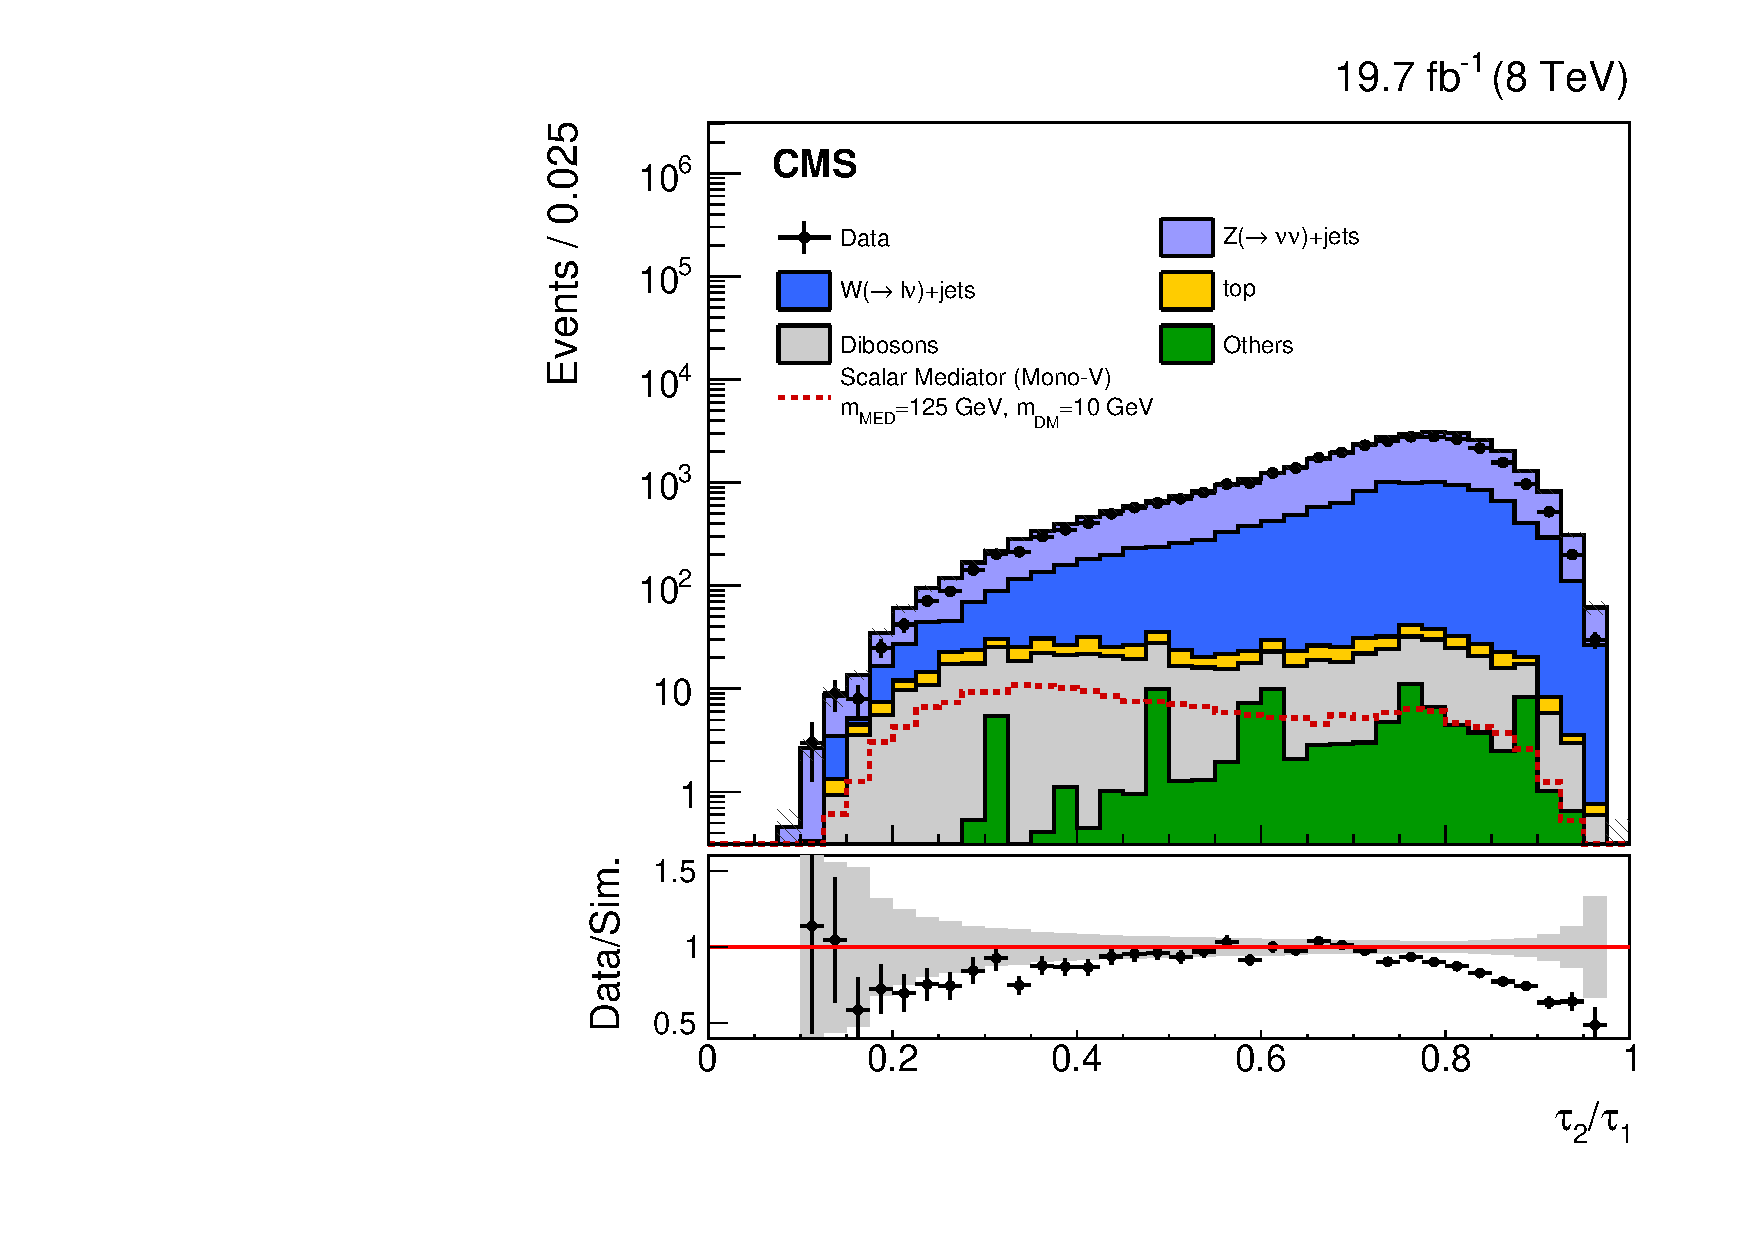
\includegraphics[width=0.49\textwidth]{figures/t2t1_sig_baseline.pdf} }
\subfigure[]{
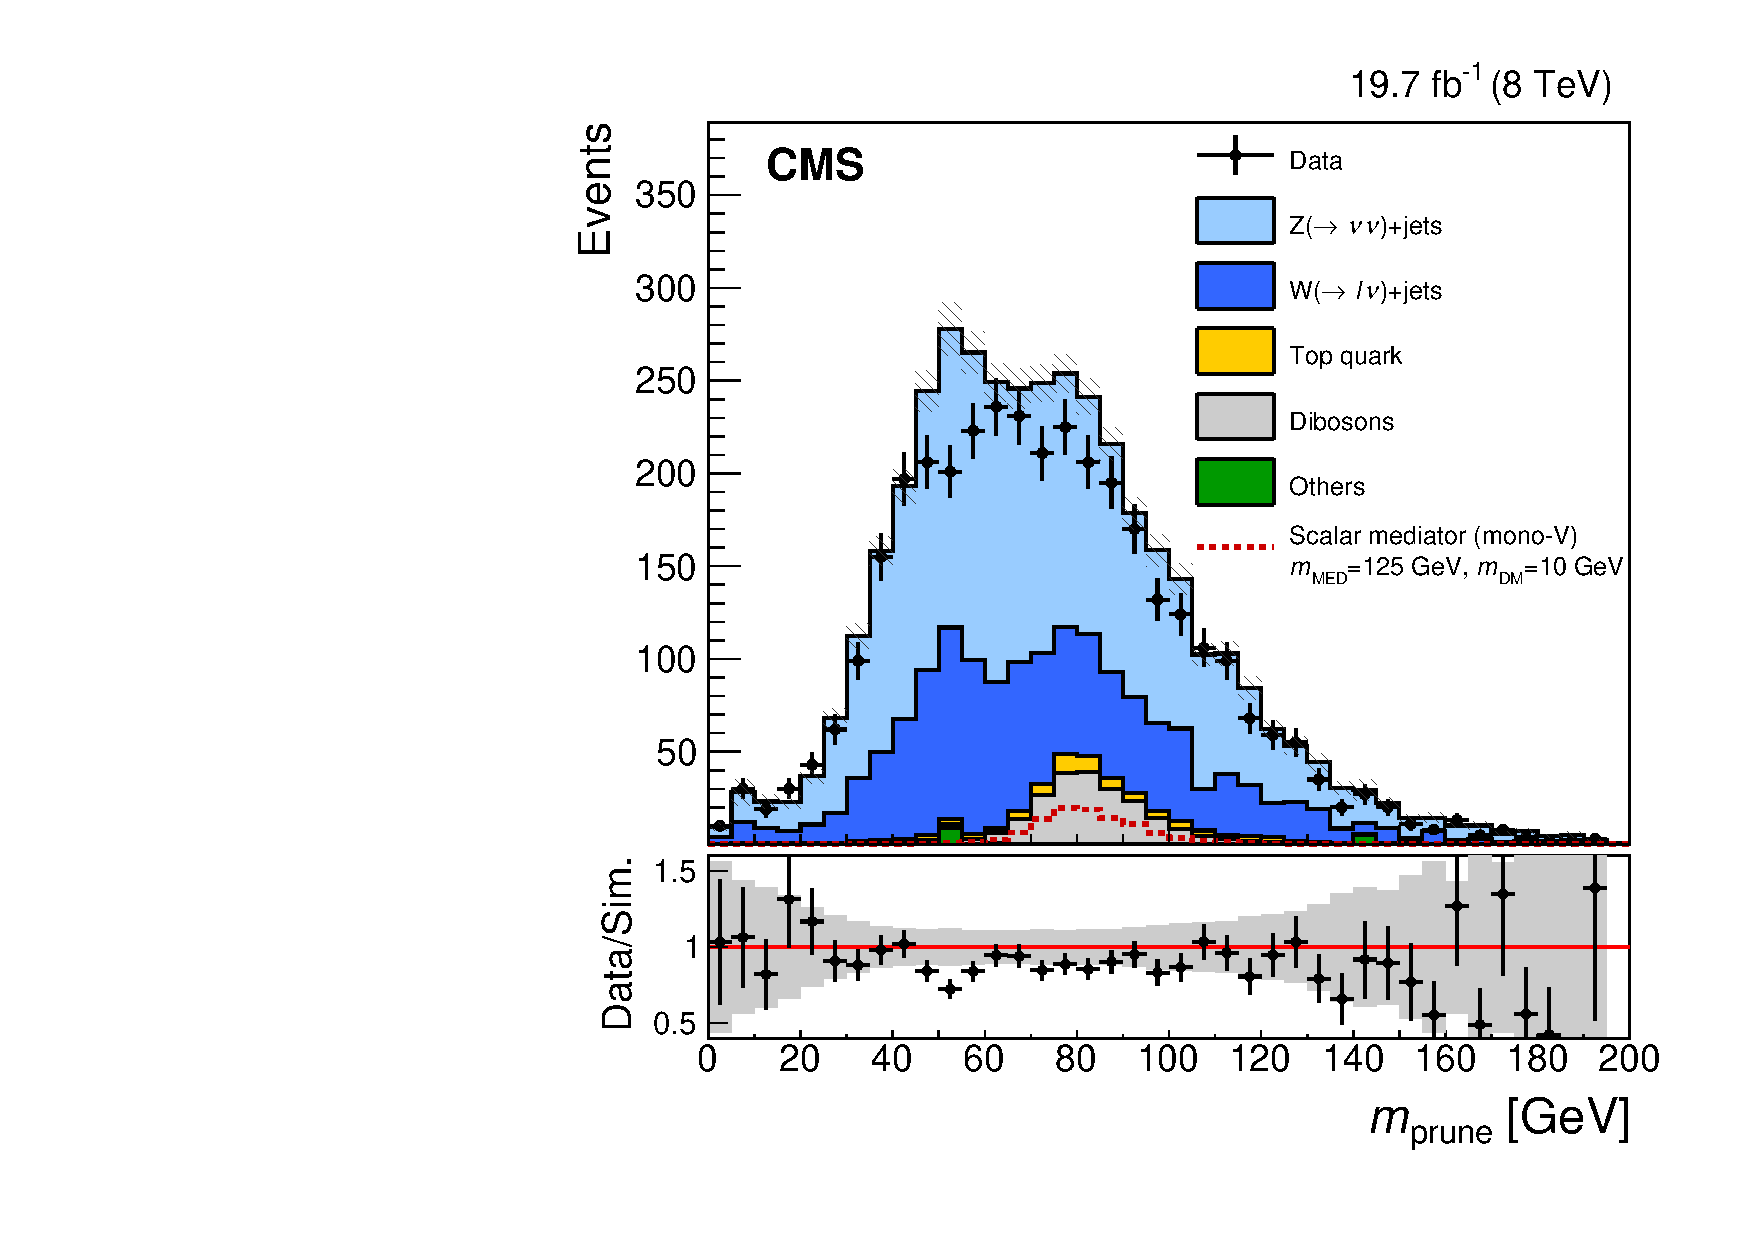
\includegraphics[width=0.49\textwidth]{figures/mass_sig_nomasscut.pdf} }
\caption{
Distributions in Lorentz-boosted events before the jet mass selection of (a) $\tau_2/\tau_1$ 
and (b) $m_{\mathrm{prune}}$ for ca8 jets. A requirement of $\tau_2/\tau_1 < $ 0.5 has been applied in (b). 
The discrepancy between data and simulation is covered by systematic uncertainties (not shown). 
The dashed red line shows the expected distribution for scalar-mediated DM production with 
$m_{\mathrm{DM}} = 10$\GeV and $m_{\mathrm{MED}} = 125$\GeV. The gray bands in the bottom panels 
indicate the statistical uncertainty from the limited number
of simulated events.}
\label{fig:boostvtagvars}\end{center}\end{figure*}

In cases where the electroweak boson has insufficient boost for
its hadronic decay to be fully contained in a single reconstructed fat jet, a
selection that looks for decays into a pair of ak5 jets is applied to recover
the event if it fails the V-boosted selection.  The selection requires that each jet
has $\pt>30$\GeV and $|\eta|<2.5$ and that the dijet has a mass in the range 
$60-110$ \GeV, consistent with originating from a W or Z boson. To further reduce
the combinatorial background in the V-resolved category, a multivariate (MVA)  
selection criterion is applied. The inputs to the MVA are the likelihood-based discriminators which distinguish 
quark from gluon jets~\cite{JME-14-002}, the jet pull angle~\cite{Gallicchio:2010sw} 
and the mass drop variable~\cite{Izaguirre:2014ira}. In events where multiple dijet pairs are
found, the pair with the highest MVA value is taken as the candidate. The
distribution of the MVA variable for SM backgrounds and for a scalar
mediator produced in association with either a W or Z boson is shown in
Fig.~\ref{fig:vtagger}. Events are selected in the V-resolved category in they have an 
MVA value greater than 0.6.

\begin{figure*}[hbtp]\begin{center} \subfloat[][]{
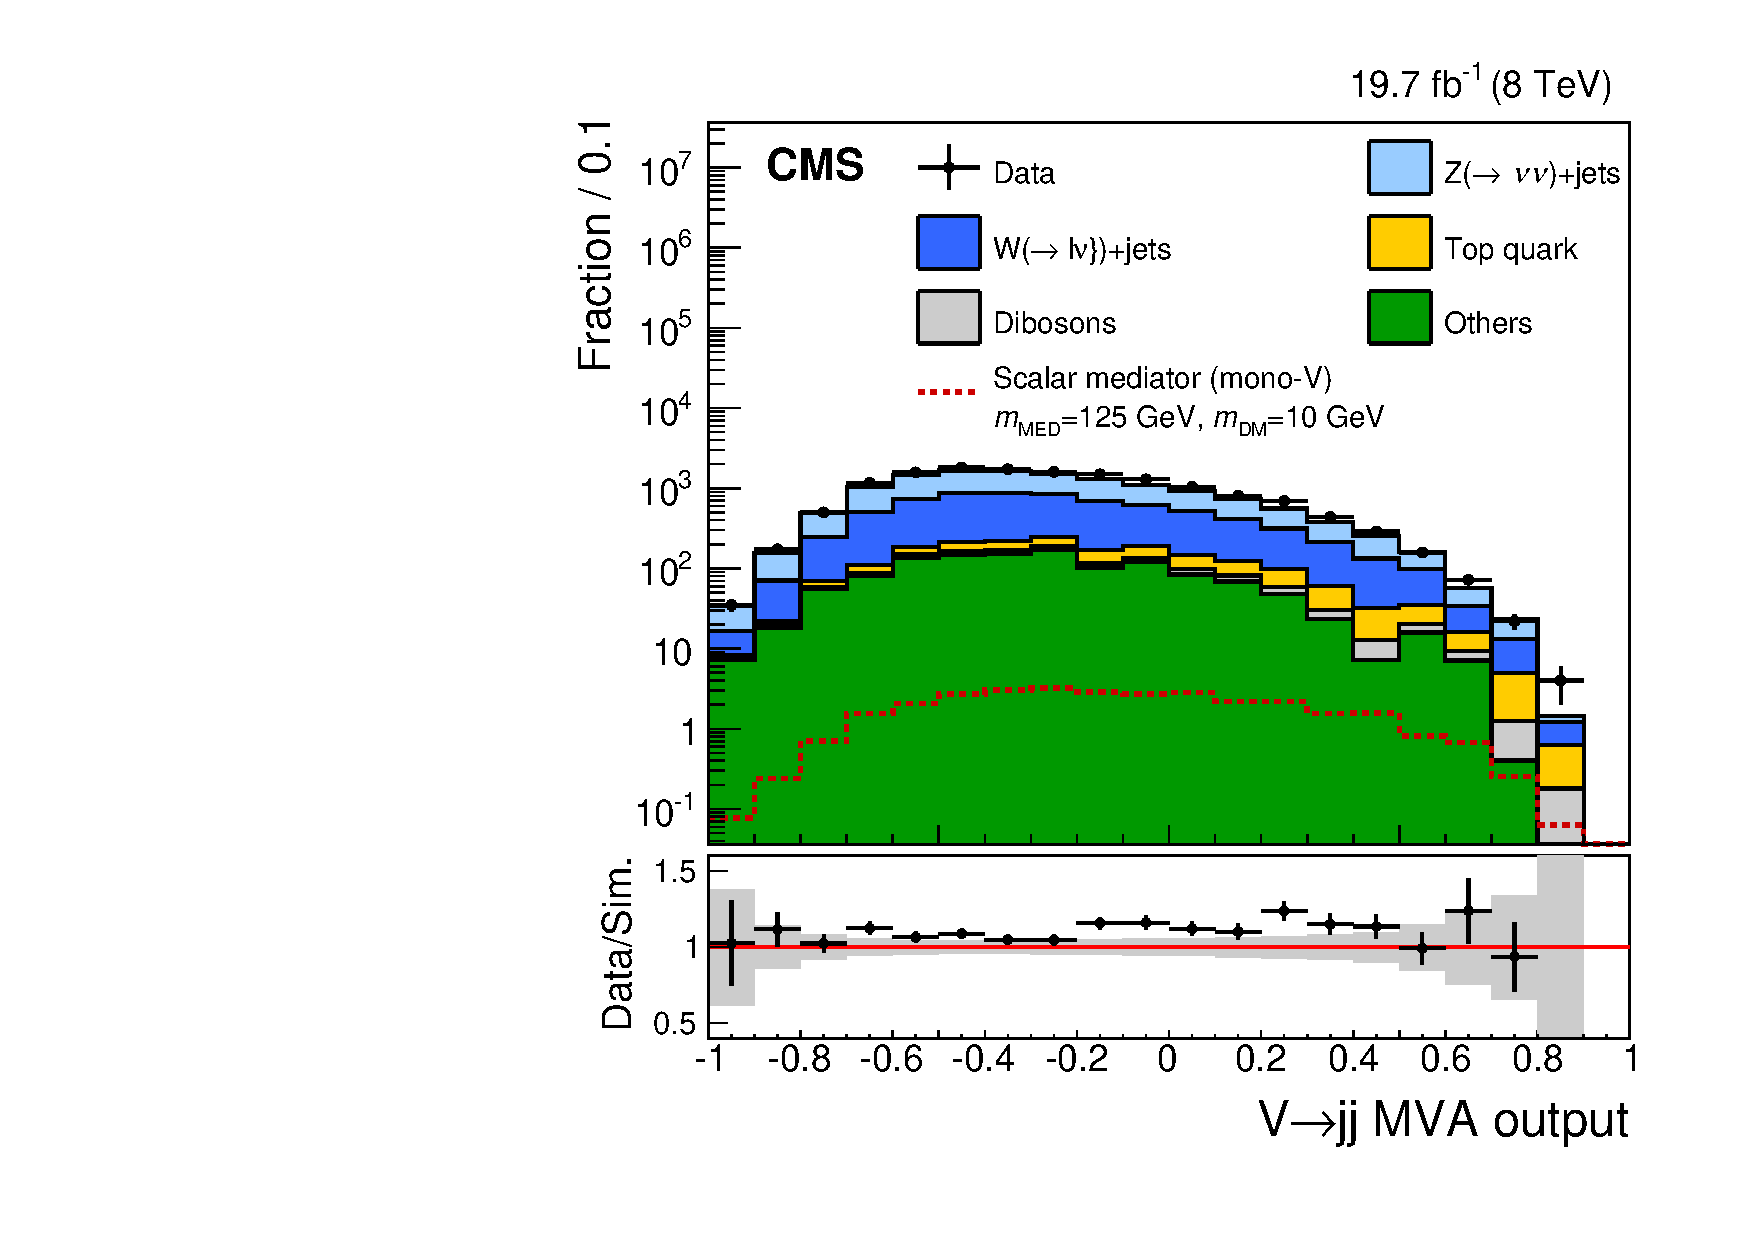
\includegraphics[width=0.49\textwidth]{figures/res_vmvalog_0.pdf} }
\subfloat[][]{ 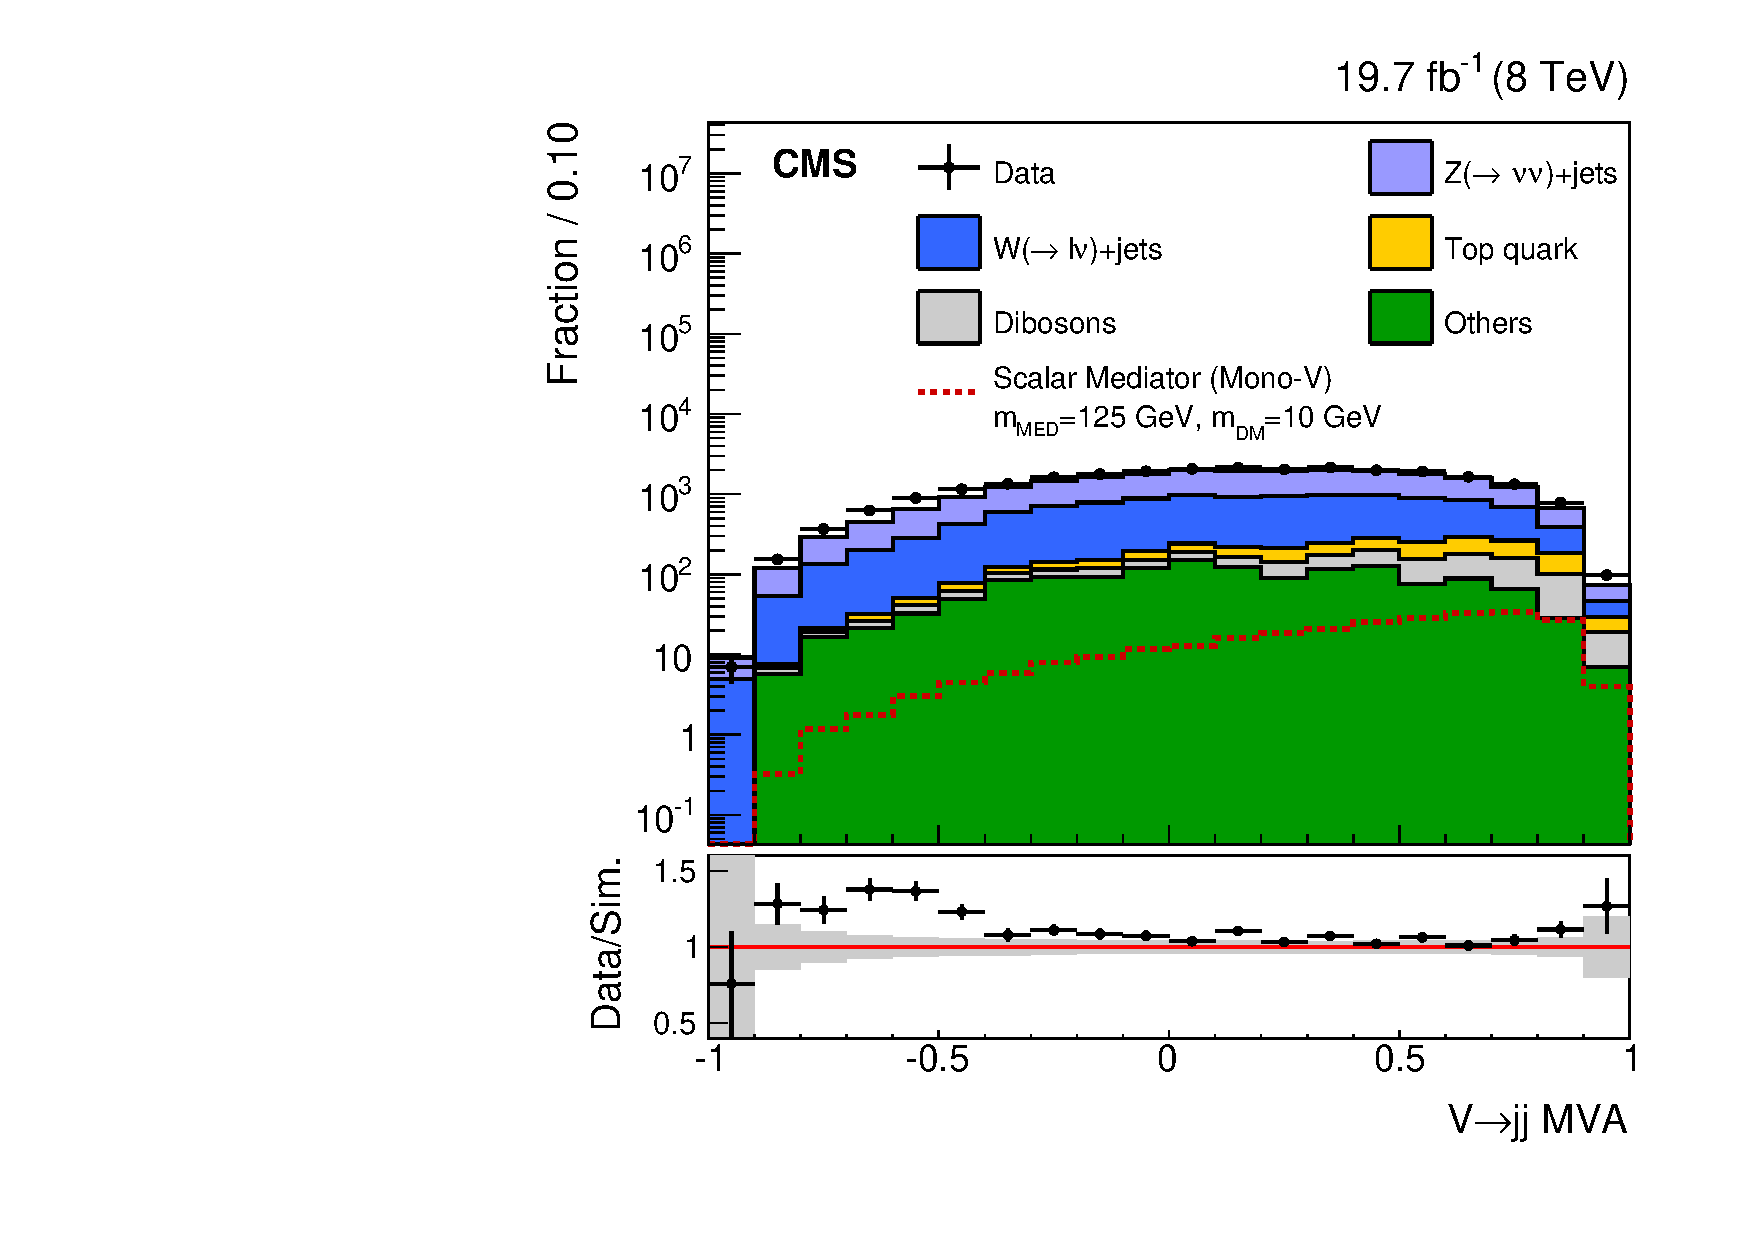
\includegraphics[width=0.49\textwidth]{figures/res_vmvalog_1.pdf}
} \caption{ 
The MVA distribution for V-tag events in simulation and data after signal selection for 
(a) $\pt < 160$ GeV and (b) $\pt > 160$ GeV. At a $\pt$ of about 160 GeV, 
the jets begin to overlap. The dashed red line shows the expected distribution 
for scalar-mediated DM production with $m_{\mathrm{DM}} = 10$\GeV and $m_{\mathrm{MED}} = 125$\GeV. 
The gray bands in the bottom panels indicate the statistical uncertainty from the limited number
of simulated events.}\label{fig:vtagger}\end{center}\end{figure*}

To reduce contamination from top quark backgrounds, events are rejected if they
contain a b-tagged jet, defined using an MVA containing secondary
vertex information and operated a medium working point  (``CSV
medium'')~\cite{BTAG}. Finally, the events are required to have $\ETm>250$ \gev. 

The events that do not qualify for either of the two V-tagged categories are
required to have one or two high \pt jets showing characteristics indicative of
originating from a \emph{single} quark or gluon. This final category is referred to 
herein as the monojet category. For the monojet category, at
least one ak5 jet within $|\eta|<2.0$ with \pt greater than 150 \GeV and a \ETm
greater than 200 \GeV is required.  As in the V-boosted category, events with a
second ak5 jet close to the leading one ($\Delta\phi(\textrm{j_1,j_2}) < 2$ radians) with
$\pt>30$\GeV and $|\eta|<2.5$ are selected to allow the frequent cases where
initial state radiation yields two jets.  Events with three or more ak5 jets
with $\pt>30$ \GeV and $|\eta|<2.5$ are rejected. Table~\ref{tab:selection} gives a 
summary of the event selection in the three categories. 


\begin{table}[h!]
	\caption{Event selections for the V-boosted, V-resolved and monojet categories
	The requirements 
	on $\pt^{\mathrm{j}}$ and $|\eta|^{\mathrm{j}}$ refer to the highest $\pt$ ca8 or ak5 jet in the 
        V-boosted or monojet categories, and to both leading ak5 jets in the V-resolved category.
	The priority for event selection is that events are first selected in the V-boosted, followed by the 
	V-resolved and finally the monojet. Events which pass a given selection are not allowed to enter a subsequent category.}
 \label{tab:selection}
 \begin{center} 
 \begin{tabular}{l|c c c}
 				     & V-boosted  & V-resolved & Monojet   \\ 
 \hline
 \hline
  $\pt^{\mathrm{j}}$     	     & $>200$\GeV & $>30$\GeV  & $>200$\GeV  \\
  $|\eta|^{\mathrm{j}}$     	     & $<2.5$\GeV & $<2$       & $<2$  \\
  $\ETm$     		     	     & $>250$\GeV & $>250$\GeV & $>200$\GeV  \\
  $\tau_2/\tau_1$      		     &  $<0.5$          & -           & - \\
  $\mathrm{V}\rightarrow{\mathrm{jj}}$ MVA    &  -               & $>0.6$      & - \\
  $m_{\mathrm{prune}}/m_{\mathrm{jj}}^{1}$    & $60-110$\GeV & $60-110$\GeV & -  \\
  $\Delta\phi(\ETm,\mathrm{j})$      	     & $>2$ rad     & -  & $>2$ rad \\
  $\mathrm{N}_{\mathrm{j}}^{2}$      & $=1$     & -  & $=1$ \\
 \hline
 \end{tabular}
 \end{center}\\
\footnotesize{$^{1}$ The cut on the mass refers to $m_{\mathrm{prune}}$ in the V-boosted category and 
the dijet invariant mass $m_{\mathrm{jj}}$ in the V-resolved category.}\\ 
\footnotesize{$^{2}$ An additional jet is allowed only if it falls within $\Delta\phi<2$ radians of the 
leading ak5 or ca8 jet for the monojet or V-boosted category. The additional ak5 jets in the V-boosted category 
must be further than $\Delta R>0.5$ for the event to fail this criteria.}
\end{table}

Figure~\ref{fig:ptandmet} shows the \ETm and leading jet $\pt$ distributions
in data and simulation after selection for all three event classes combined. The
backgrounds are normalized to full data integrated luminosity (19.7\fbinv) and the expected distribution for
vector mediated DM production assuming a DM mass of 10~\GeV and mediator mass of
1~\TeV is shown.  The discrepancy between the data and simulation is a result of
both detector resolution mismodelling and an imperfect theoretical
description of the kinematics of the W/Z+jet processes.  Both effects are
corrected for in this analysis using a control samples in data described in the
following section. 

\begin{figure*}[hbtp]\begin{center} \subfloat[][]{
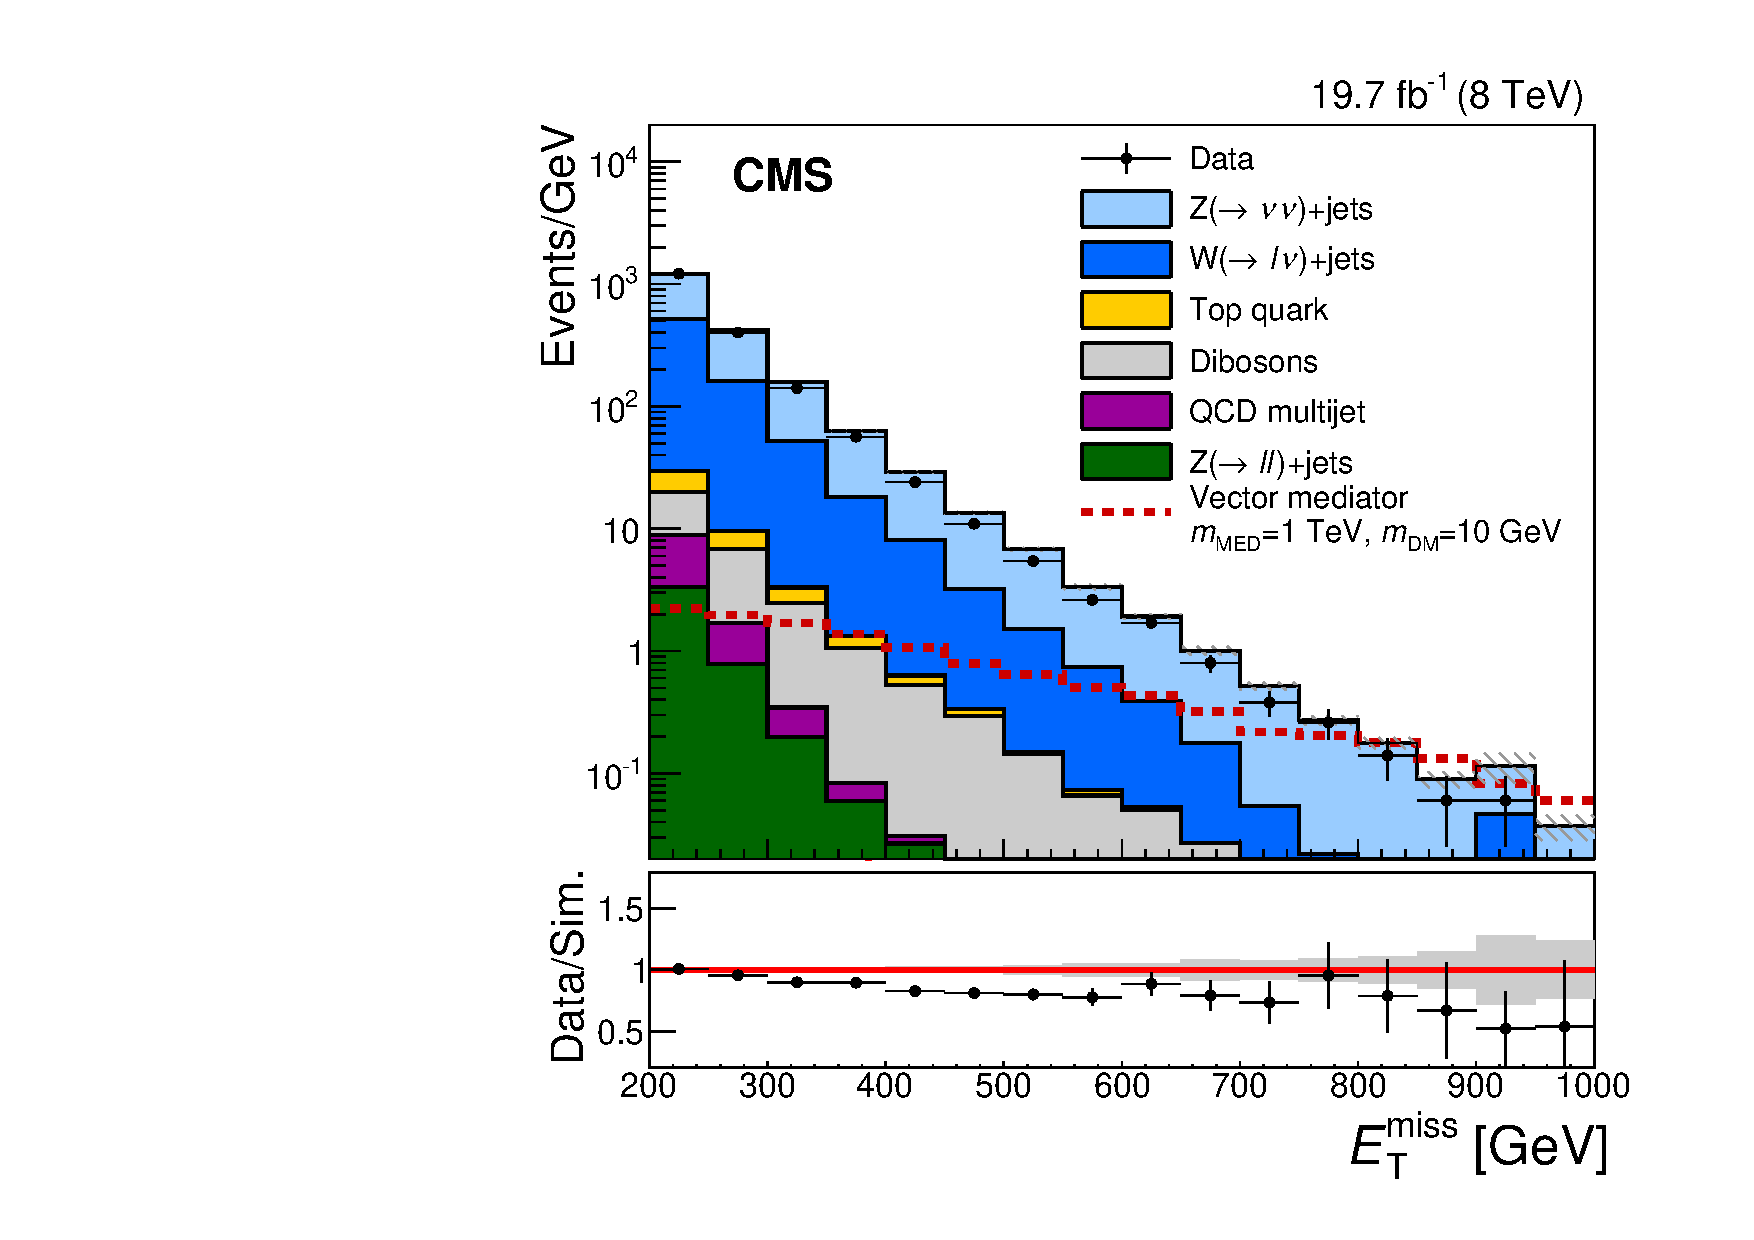
\includegraphics[width=0.49\textwidth]{figures/plot_config_combsignal_category_monojet.pdf}
} \subfloat[][]{
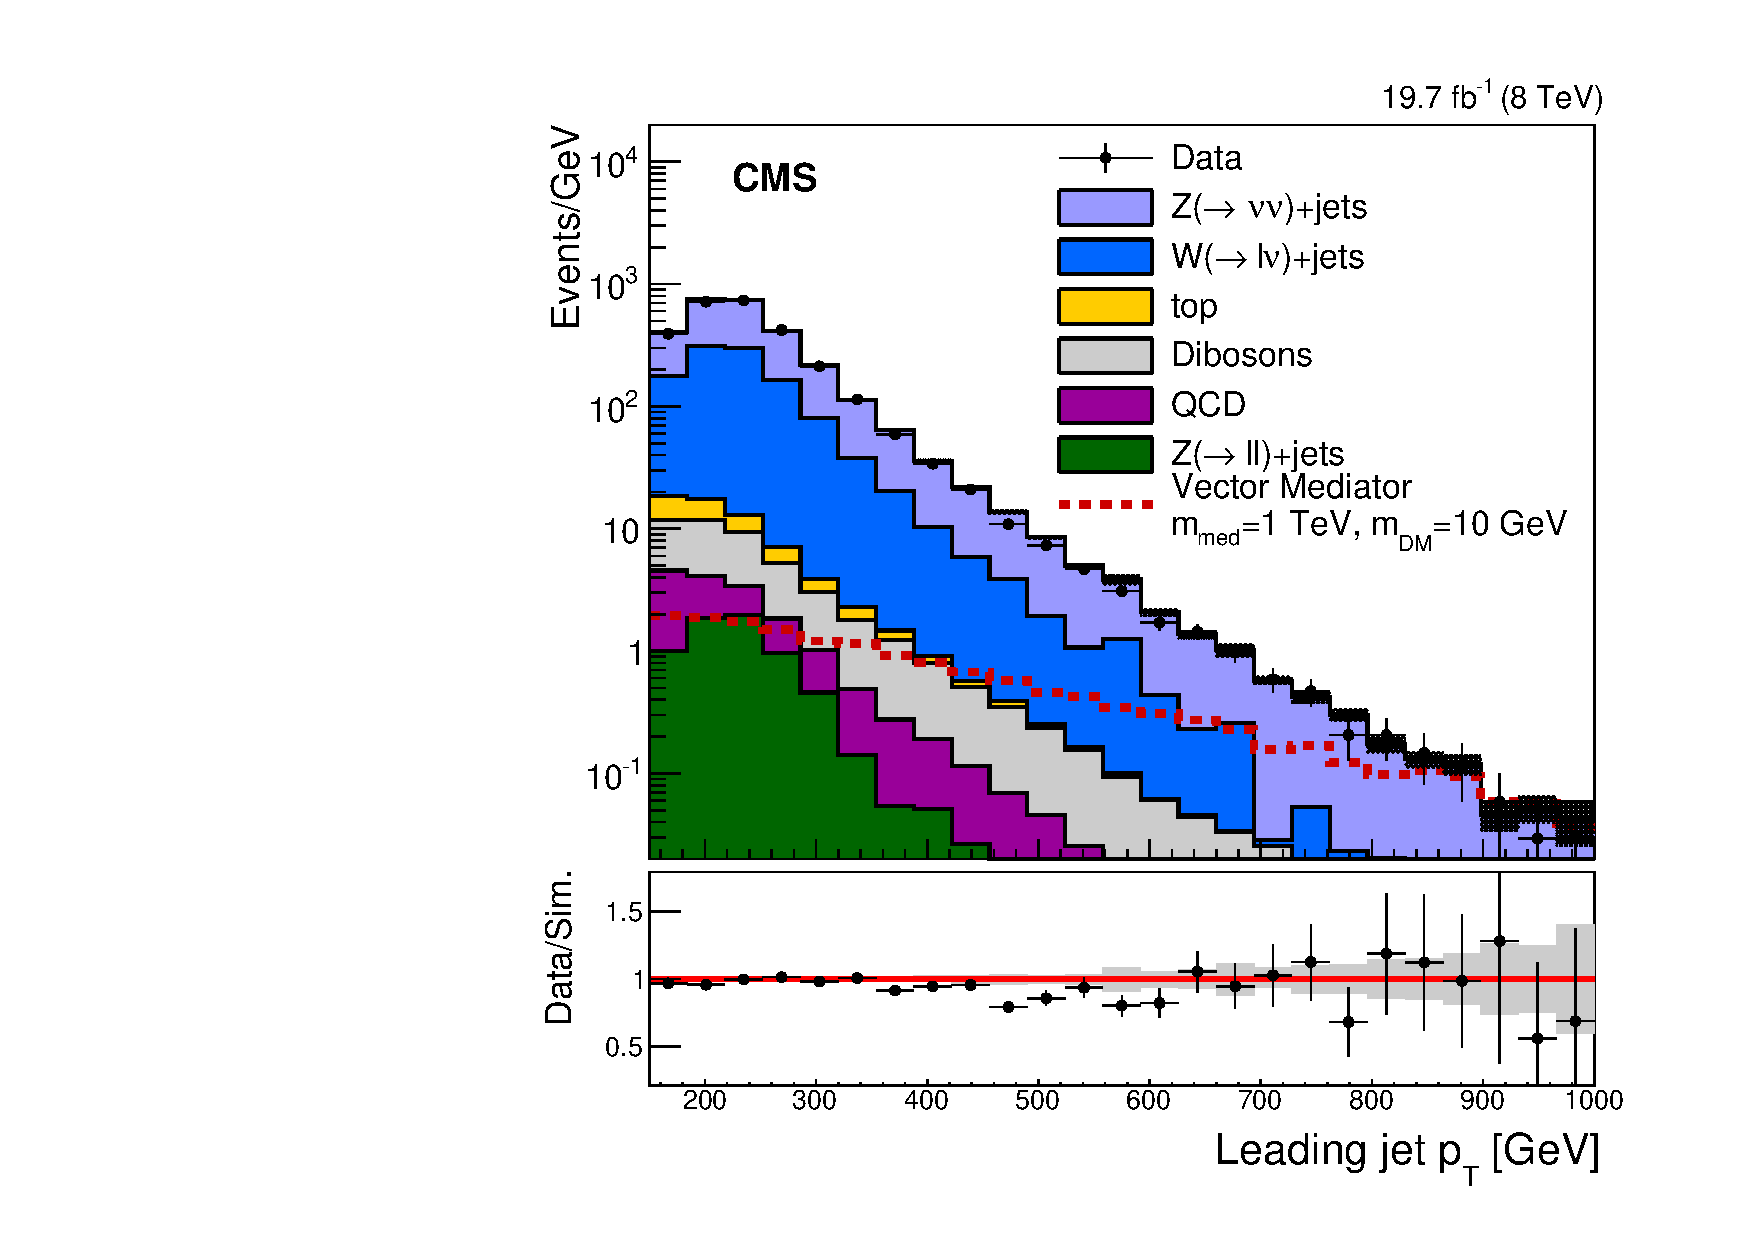
\includegraphics[width=0.49\textwidth]{figures/plot_config_combsignal_jpt_category_monojet.pdf}\\
} \caption{ Distributions of  (a) \ETm and (b) leading jet $\pt$ in simulated
events and data, after the signal selection for all three event categories
combined. The dashed red line shows the expected distribution assuming vector
mediated DM production with $m_{\mathrm{DM}}=10$\GeV and $m_{\mathrm{MED}}=1$ TeV.  
The gray bands in the bottom panels indicate the statistical uncertainty from the limited number
of simulated events.} \label{fig:ptandmet}\end{center}\end{figure*}


\section{Background estimation}

The presence of DM production will be observable as an excess of events above SM 
backgrounds at high $\ETm$. 
Significant improvements in terms of sensitivity can be
expected if several bins in $\ETm$, yielding the $\ETm$ shape, are considered simultaneously. Further
improvement is achieved by using control regions in data to 
reduce the uncertainties on the predictions of the SM backgrounds. These regions are
statistically independent from the signal region and designed such that the expected contribution 
from a potential signal is negligible. 
A binned likelihood fit is performed in the ranges 250-1000 \GeV and 200-1000 \GeV 
for the V-tag (V-boosted and V-resolved) and monojet events, respectively. The binning is chosen to
ensure each corresponding bin of a set of control regions is populated. The
width of the highest $\ETm$ bin is chosen to provide ease of comparison to the previous
CMS search~\cite{monojet1}. 

The background contributions from \Zvvjets~(\Wlvjets)~is determined using data 
from dimuon and photon (single-muon) control regions. The dimuon control region is defined 
using the same selection as for the signal region, but removing the muon veto. Instead, exactly 
two isolated muons are required with opposite charge, $\pt^{\mu_{1},\mu_{2}}>20,10$\GeV and an 
invariant mass in the range $60-120$~\GeV. 

As the decay branching ratio of \Zmm~is approximately six times smaller than that
to neutrinos, the resulting statistical uncertainty on the \Zvvjets~background 
becomes a dominant systematic uncertainty at large values of \ETm.  A
complementary approach is to use events in data that have a high-$\pt$ photon
recoiling against jets to further constrain the \Zvvjets~background~\cite{CMS-PAS-SUS-08-002}. 
This is advantageous since the production
cross-section of \phojets~is roughly three times that of the \Zvvjets~resulting in a
smaller statistical uncertainty on the predicted background. The theoretical uncertainties 
associated to the translation of the kinematics in $\phojets$ events to that of $\Zvvjets$ events 
are however significant. A combination of both photon and dimuon control regions is therefore used 
to maximally constrain the $\Zvvjets$ background.  

The photon control region consists of events which are selected by a trigger requiring an 
isolated photon with transverse momentum greater than 150\GeV~\cite{Khachatryan:2015iwa}. 
The selected events are required to have at least one photon with $p_{\mathrm{T}} > 170~\textrm{GeV}$ and 
$|\eta|<2.5$, excluding photons in the ECAL transition region, $1.44 <
|\eta|< 1.56$. All other kinematic selections are the smae as the
signal region, where here the photon is ignored in the $\ETm$ calculation.

To estimate the $\Wlvjets$ background, a single-muon control region is defined by selecting events 
with exactly one muon with $\pt$ larger than 20\GeV. Additionally the transverse 
mass, calculated as $m_{\mathrm{T}}=\sqrt{2\ETm p_{\mathrm{T}}^{\mu} (1-\cos \phi)}$, where $\phi$ 
is the azimuthal angle between the muon and $\ETm$ vector, must satisfy $50<m_{\mathrm{T}}<100$ \GeV.

The events in the control regions are
divided into the three  categories, using the same selection criteria
described in Section~\ref{sec:selection}, but in addition requiring the presence
of a pair of oppositely charged muons consistent with a Z boson decay, a high
$p_{\mathrm{T}}$ photon or a single muon consistent with a leptonic W boson decay.
In the control regions, the momenutm of the dimuon pair,
single-muon or the photon is removed and the \ETm~is recalculated
yielding a distribution of fake \ETm. The distribution of fake \ETm~in 
the control regions is used to derive the expectation from the \Zvvjets~and \Wlvjets~
backgrounds in the signal region.

 
The \ETm spectra of the $\vjets$ backgrounds are determined through the
use of the binned likelihood fit, simultaneously across all bins in the three control regions.
The expected number of events $N_{i}$ in a given bin $i$ of fake \ETm, for a
particular event category, is given by $N^{{\rm Z}_{\mu\mu}|\gamma }_{i}=
\dfrac{{\mu^{\Zvv}_{i}}}{R^{{\rm Z}|\gamma}_{i}}$ for the dimuon and photon control
regions and  $N^{\rm W}_{i} =  \dfrac{{\mu^{\Wlv}_{i}}}{R^{\rm W}_{i}}$, for the
single-muon control region. The parameters $\mu^{\Zvv}$ and
$\mu^{\Wlv}$ are free parameters of the likelihood representing
the yields of $\Zvvjets$ and $\Wlvjets$ in each bin of the signal region. The
additional terms $R^{\rm W}_{i}$, $R^{{\rm Z}|\gamma}_{i}$ denote factors which
account for the extrapolation of specific backgrounds from the signal region to 
control regions. The likelihood function for a particular category is
given by   

\begin{align*}
\mathcal{L}(\boldsymbol{\mu}^{\Zvv},\boldsymbol{\mu}^{\Wlv},\boldsymbol{\beta},\boldsymbol{\alpha})
&=        \prod_{i} \mathrm{Poisson}\left(d^{\gamma}_{i}
|B^{\gamma}_{i}(\boldsymbol{\alpha}) +\frac{ \mu^{\Zvv}_{i}
}{R^{\gamma}_{i}(\boldsymbol{\beta})}   \right) \\ &~\times
\prod_{i} \mathrm{Poisson}\left(d^{Z}_{i}
|B^{\rm Z}_{i}(\boldsymbol{\alpha})      +\frac{ \mu^{\Zvv}_{i}
}{R^{\rm Z}_{i}     (\boldsymbol{\beta})}       \right ) \\ &~\times
\prod_{i} \mathrm{Poisson}\left(d^{W}_{i}
|B^{\rm W}_{i}(\boldsymbol{\alpha})      +\frac{ \mu^{\Wlv}_{i}
}{R^{\rm W}_{i}     (\boldsymbol{\beta})}       \right),
\numberthis\label{eqn:candclh} \end{align*}

where $d^{\gamma/{\rm Z}/{\rm W}}_{i}$ are the observed number of events in each bin of
the photon, dimuon and single-muon control regions. Additionally,
$\boldsymbol{\alpha,\beta}$ denote parameters profiled over during the
likelihood minimization, and Poisson denotes its eponymous distribution.  The expected contributions
from background processes in the photon, dimuon and single-muon control regions
are denoted $B^{\gamma}$, $B^{\rm Z}$ and $B^{\rm W}$ in Equation~\ref{eqn:candclh},
respectively.

The factors $R^{\rm Z}_{i}$ account for the ratio of $BR(\Zvv)/BR(\Zmm)$
and the muon efficiency times acceptance in the dimuon control region, while
$R^{\gamma}_{i}$ account for the ratio of differential cross section between
the $\Zjets$ and $\phojets$ processes, and the efficiency times acceptance of the
photon selection for the $\phojets$ control region. The differential cross sections 
of photon and Z production are first corrected using next-to-leading order   
K-factors derived by comparing their $\pt$ distributions in events generated
with {\sc Madgraph5\_aMC@NLO V5.2.2.2}~\cite{amcatnlo}, to the
distributions produced at leading order before deriving the factors 
$R^{\gamma}_{i}$ and $R^{\rm Z}_{i}$. 

Systematic uncertainties are modelled as constrained nuisance parameters
which allow for variation of the factors 
$R^{\gamma/Z/W}$ in the fit, and are treated as fully correlated between event
categories.  These include theoretical uncertainties on the photon to Z
differential cross-section ratio from renormalization and factorization scale
uncertainties which amount to 10\% across the relevant boson \pt range, 
when summed in quadrature. The scale uncertainties for both the renormalization
and factorization scale are treated as partially correlated between
process($\gamma/W/Z$) with a
20\% decorrelated component designed to match the maximum scale
uncertainty on each individual process.   
Electroweak corrections are not accounted for in 
the simulation. Additional K-factors are applied as a function 
of the boson (Z or $\gamma$) \pt, to account for higher order electroweak effects which are around 15\% 
for a boson \pt around 1 TeV~\cite{Kuhn:2005gv}. The full correction is taken as an uncertainty on the 
ratio. A conservative choice is made in assuming this
uncertainty to be uncorrelated across bins of \ETm. The
uncertainties in the muon selection efficiency, photon selection efficiency, and
photon purity are included and fully correlated across the event categories and
fit to the control regions are shown in Fig.~\ref{fig:combined_fit_result}.
 
\begin{figure*}[hbtp]\begin{center}
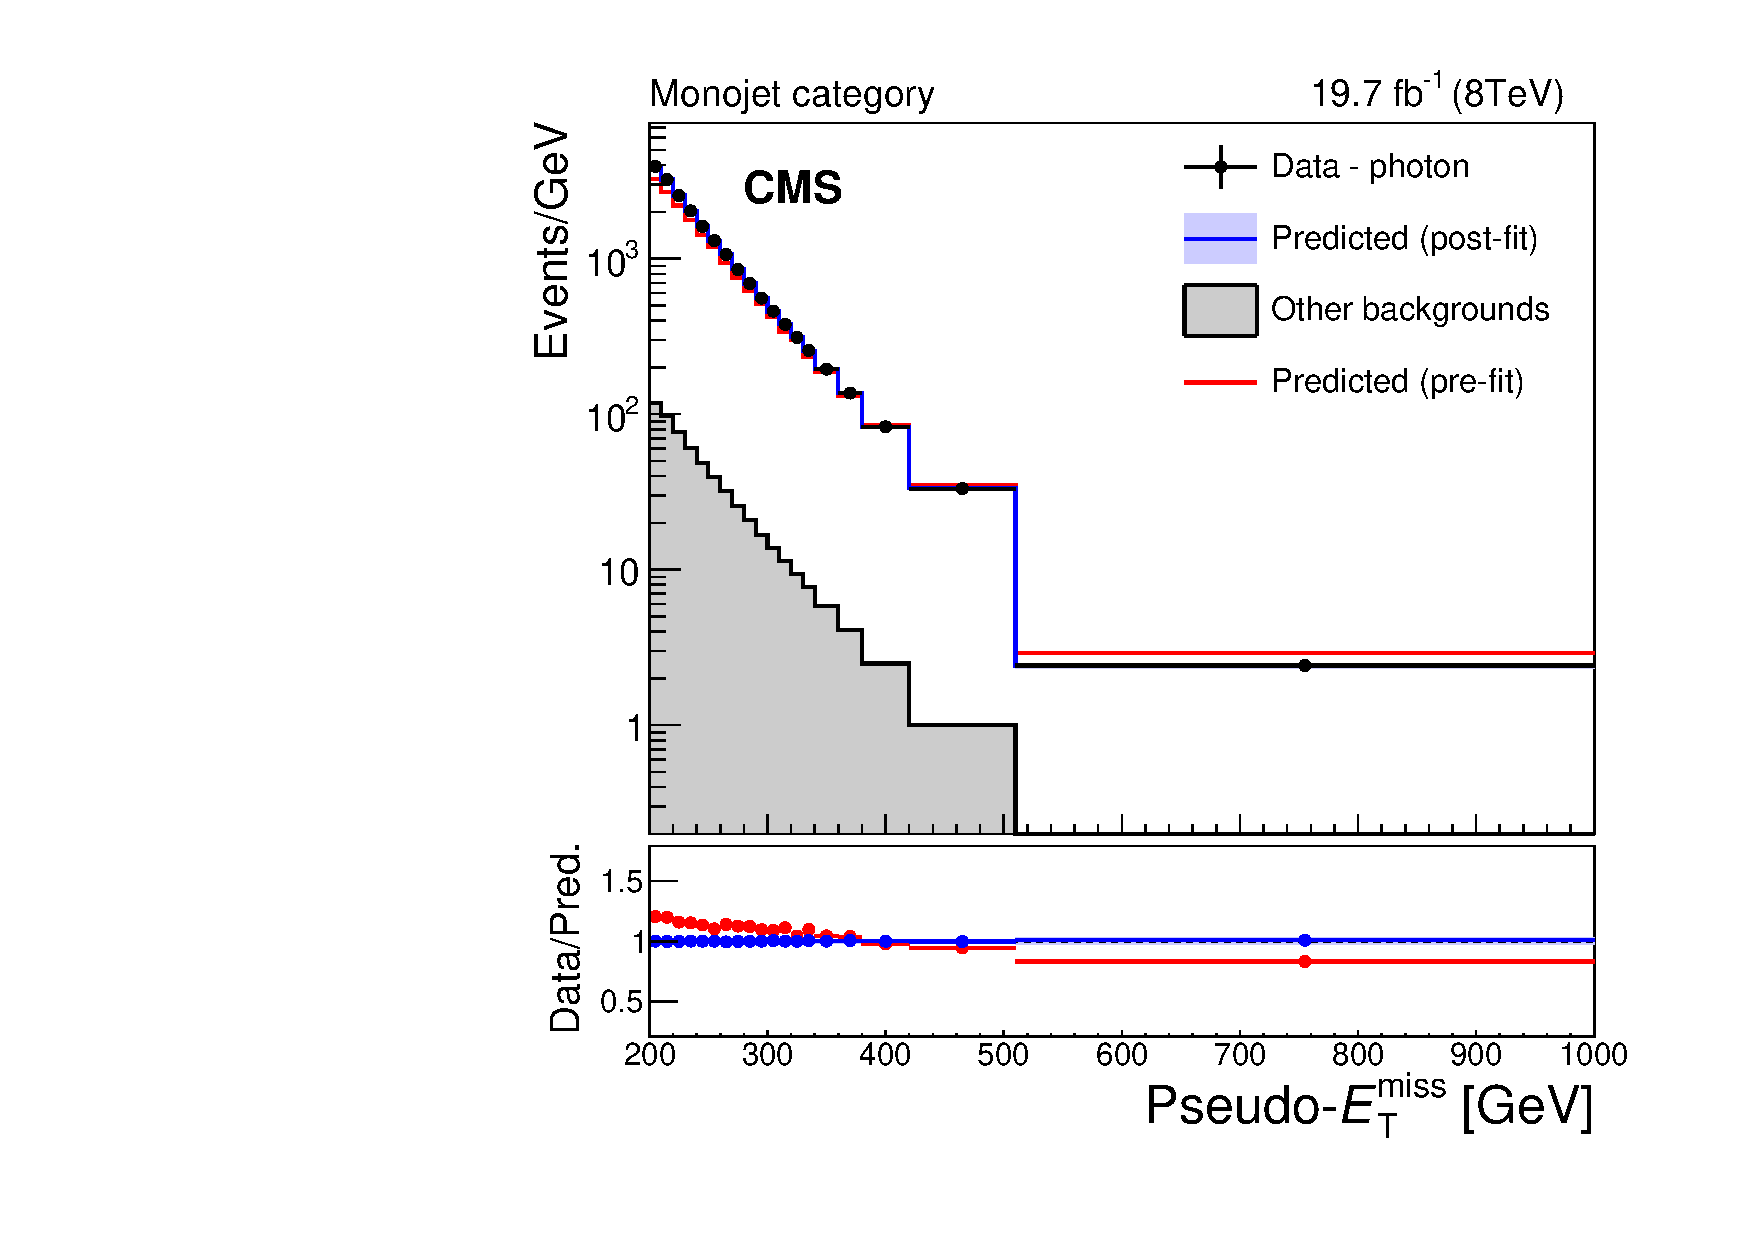
\includegraphics[width=0.32\textwidth]{figures/post_fit_photon_monojet.pdf}
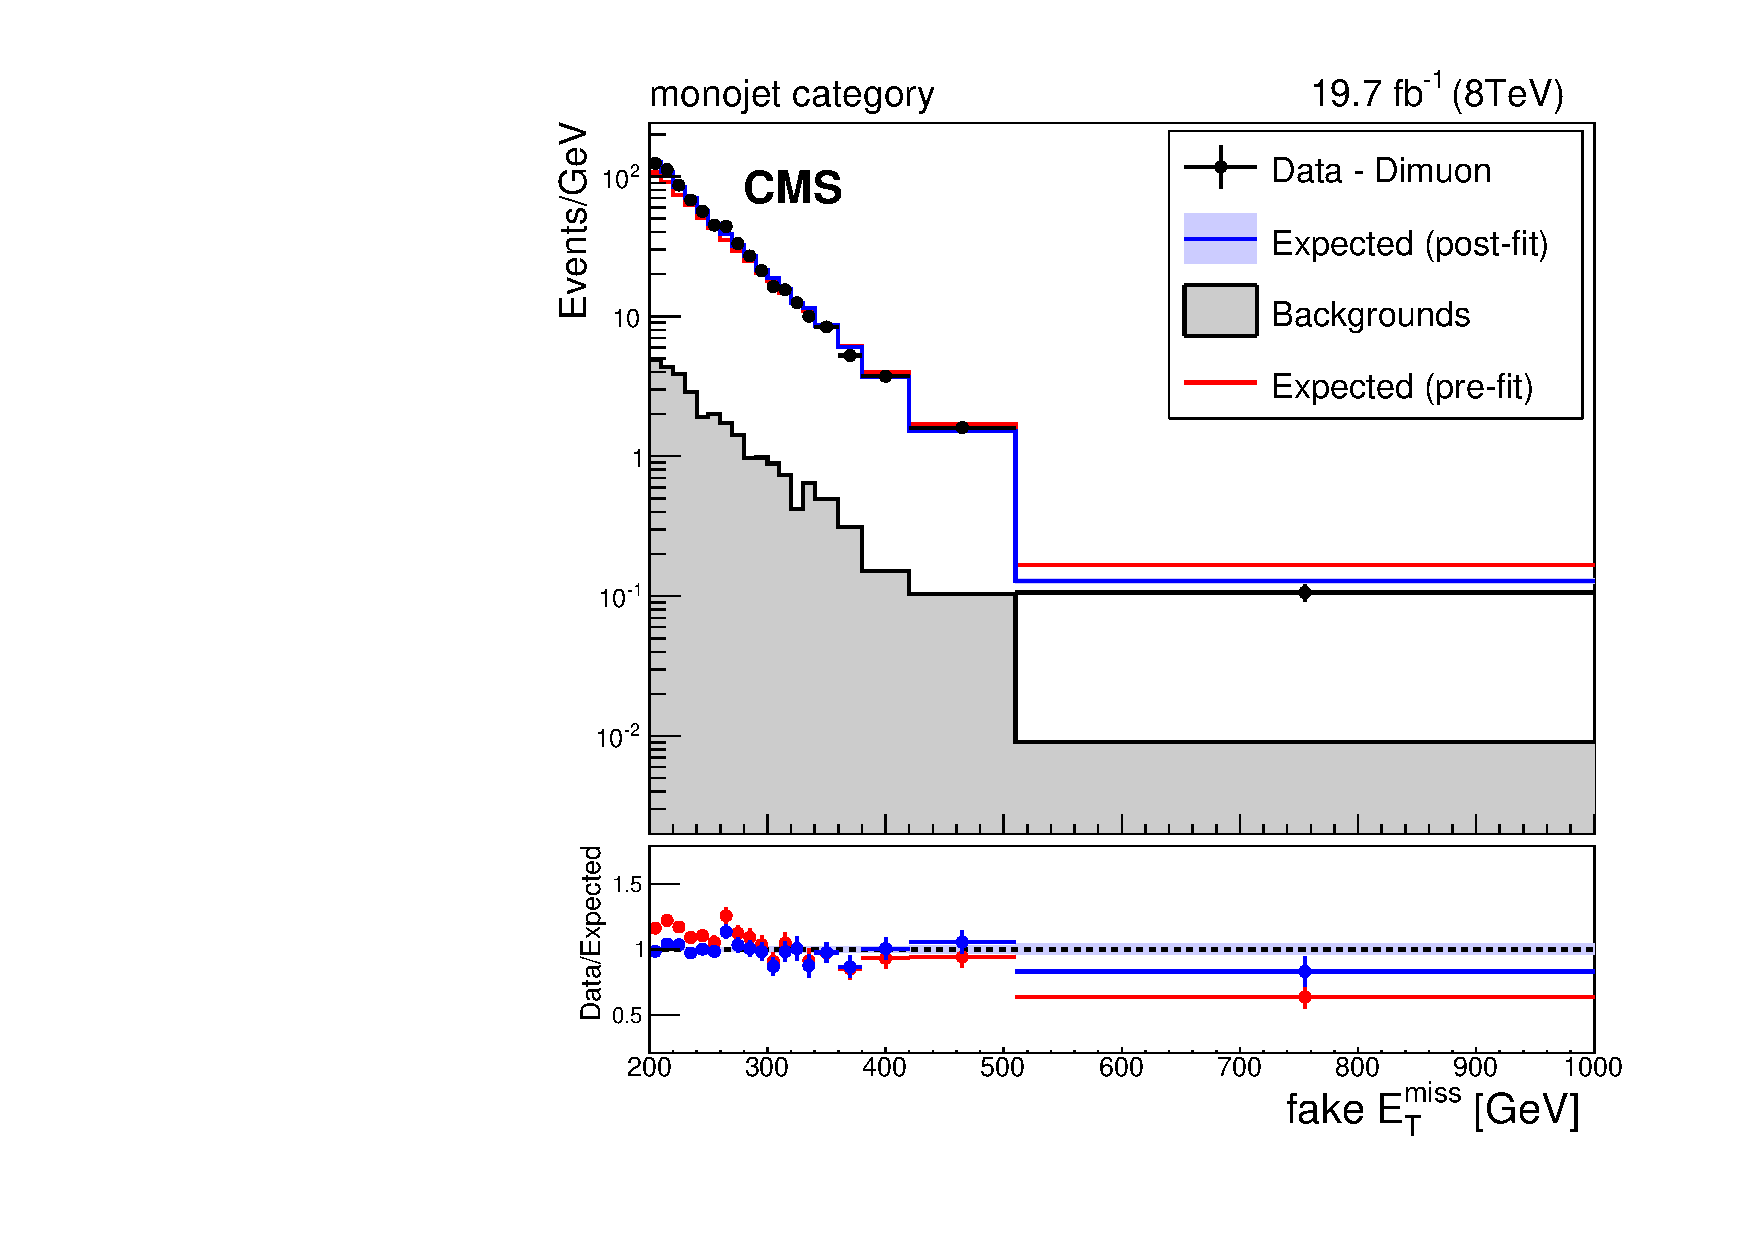
\includegraphics[width=0.32\textwidth]{figures/post_fit_zmm_monojet.pdf}
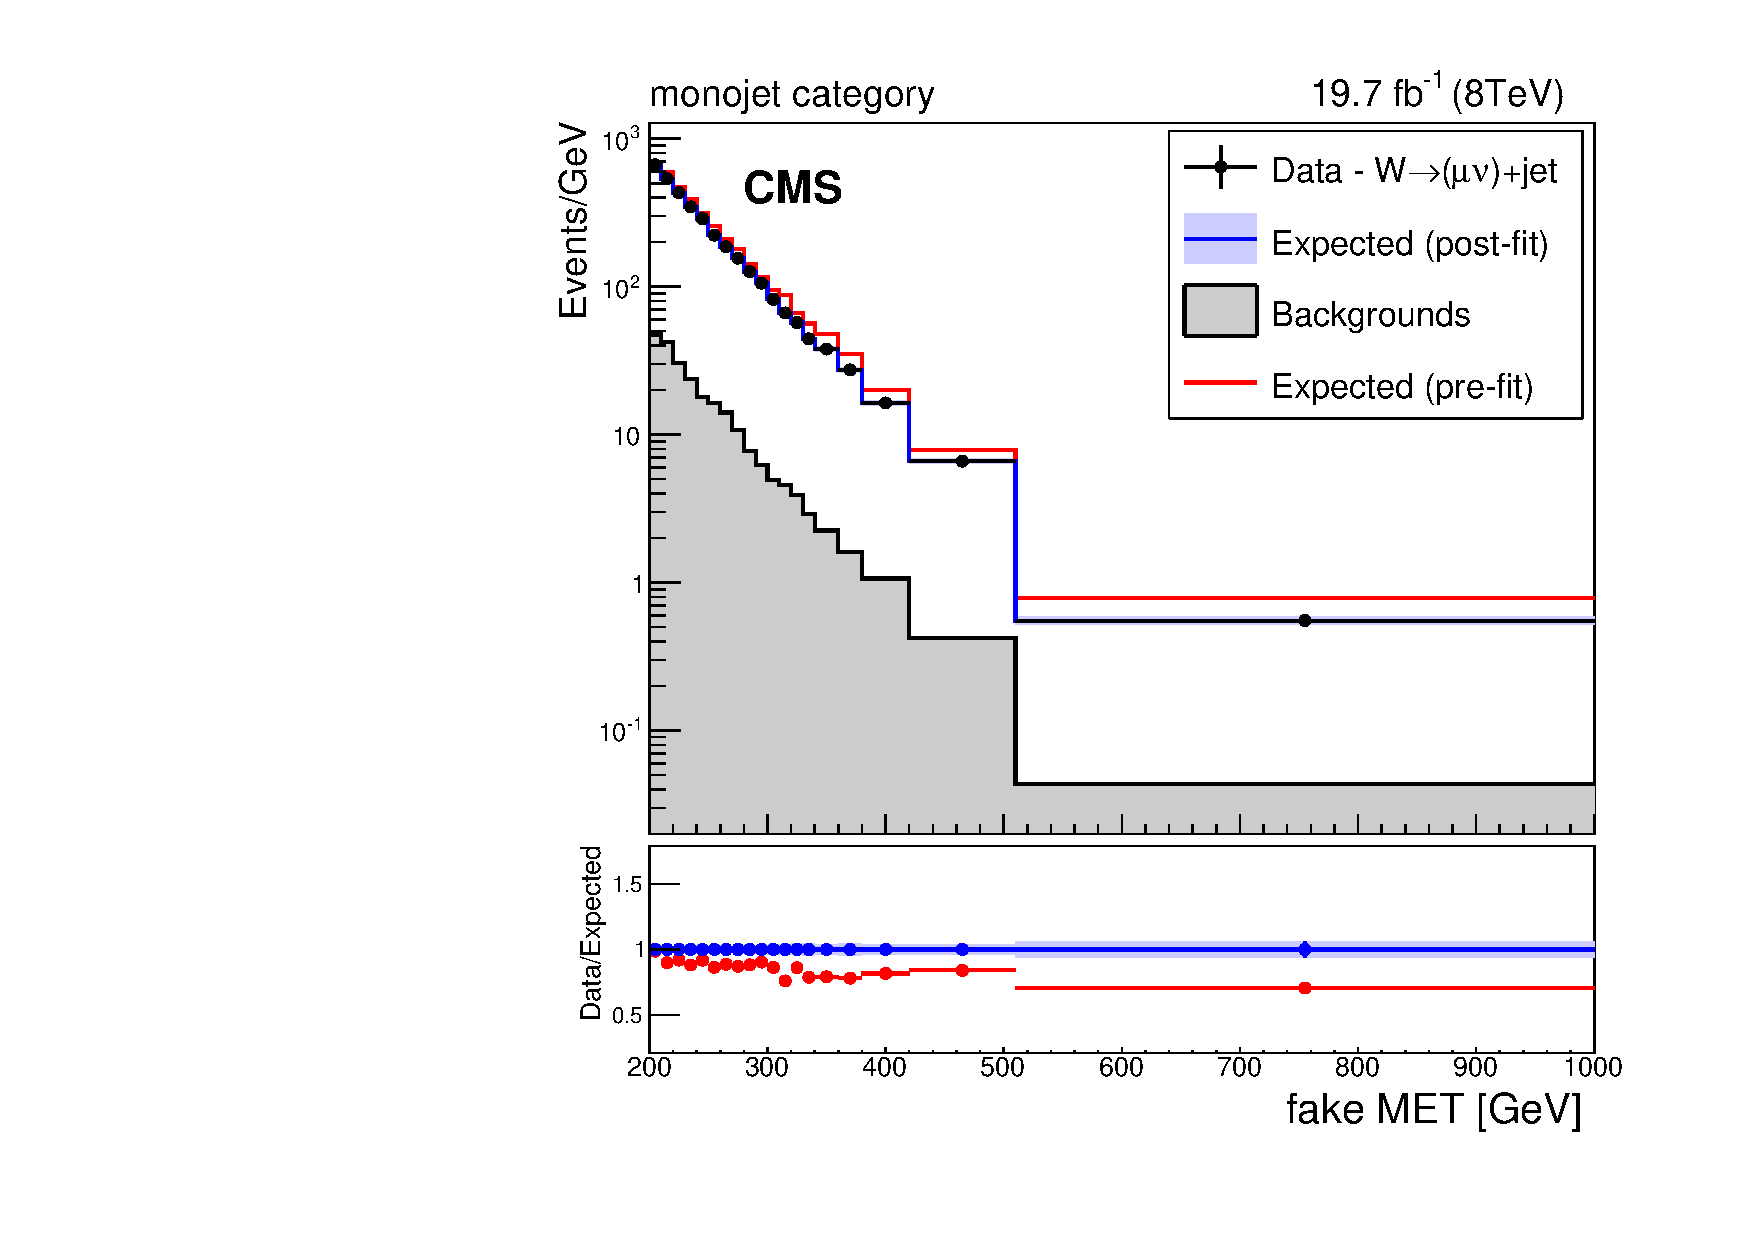
\includegraphics[width=0.32\textwidth]{figures/post_fit_wmn_monojet.pdf}\\
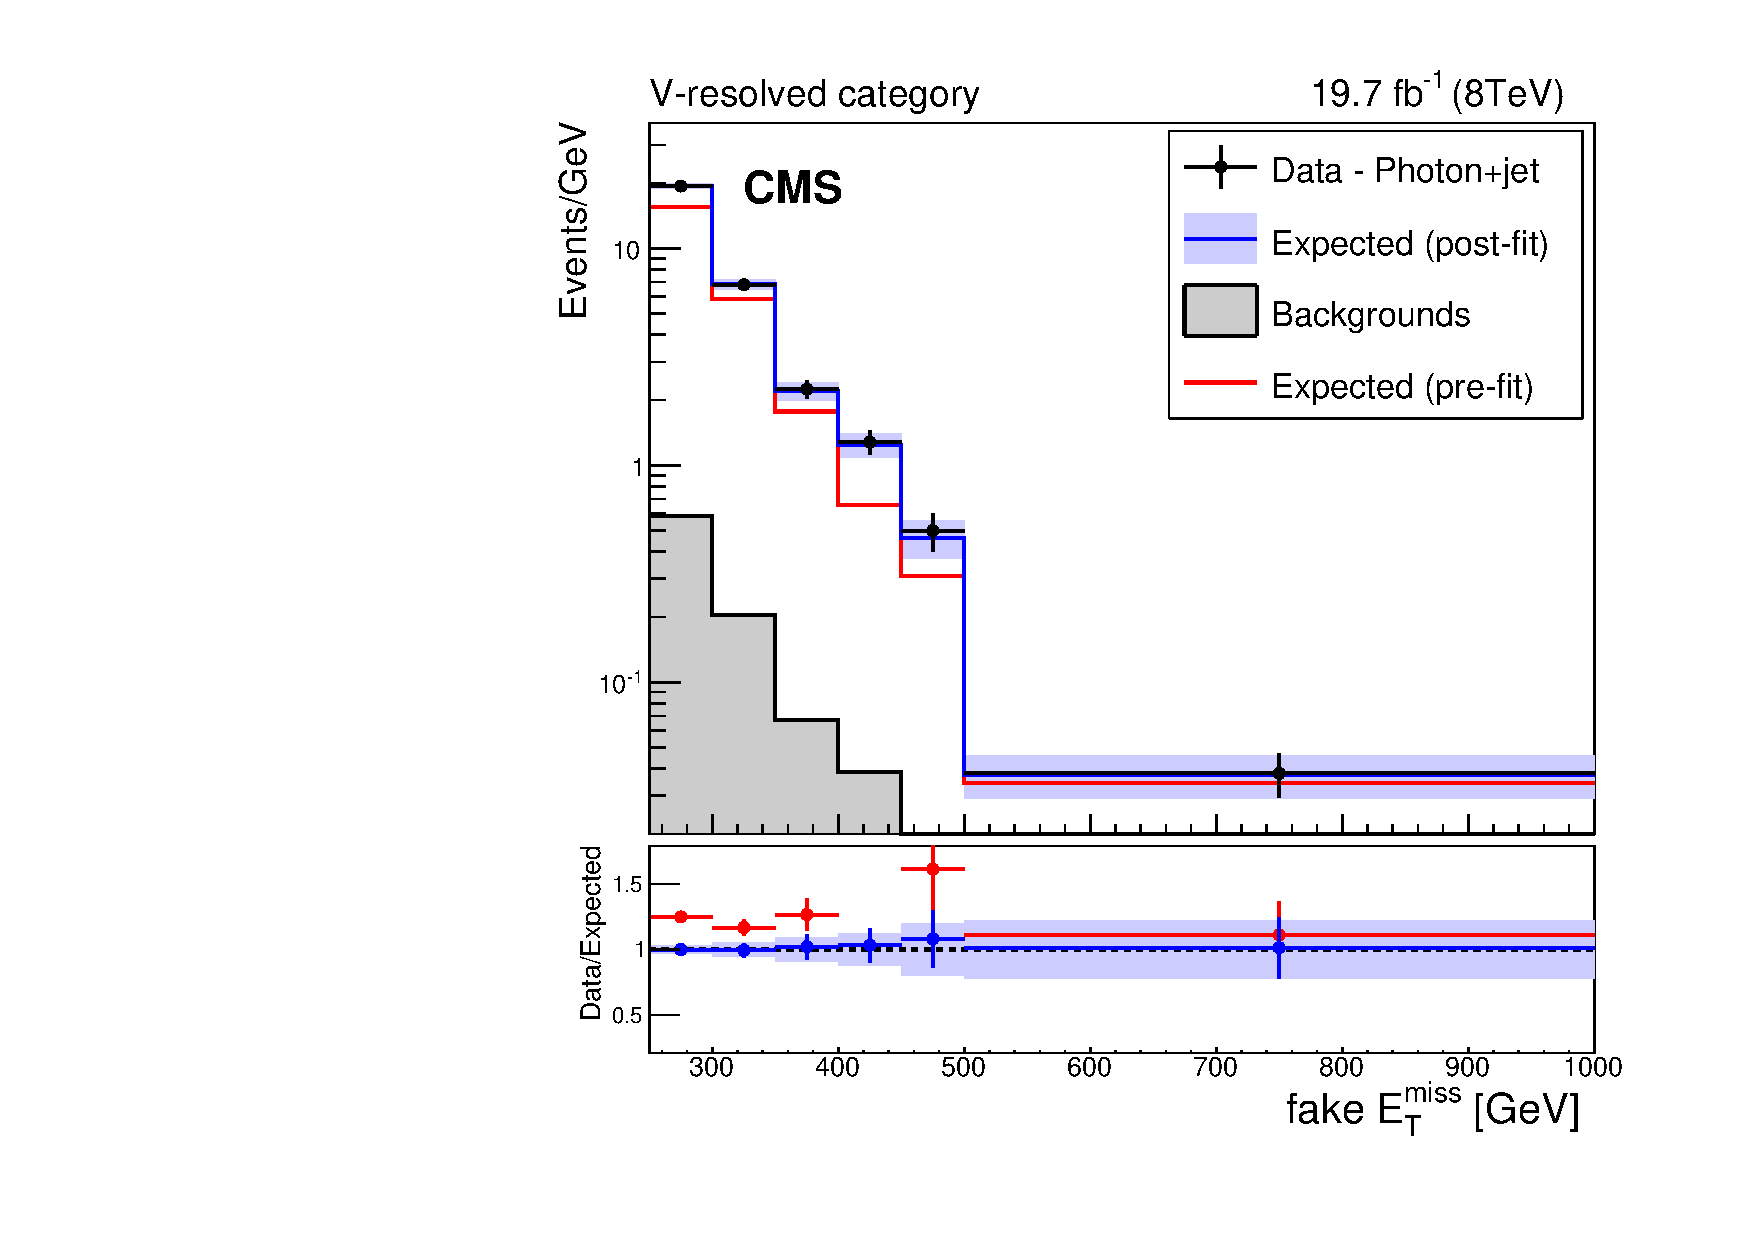
\includegraphics[width=0.32\textwidth]{figures/post_fit_photon_resolved.pdf}
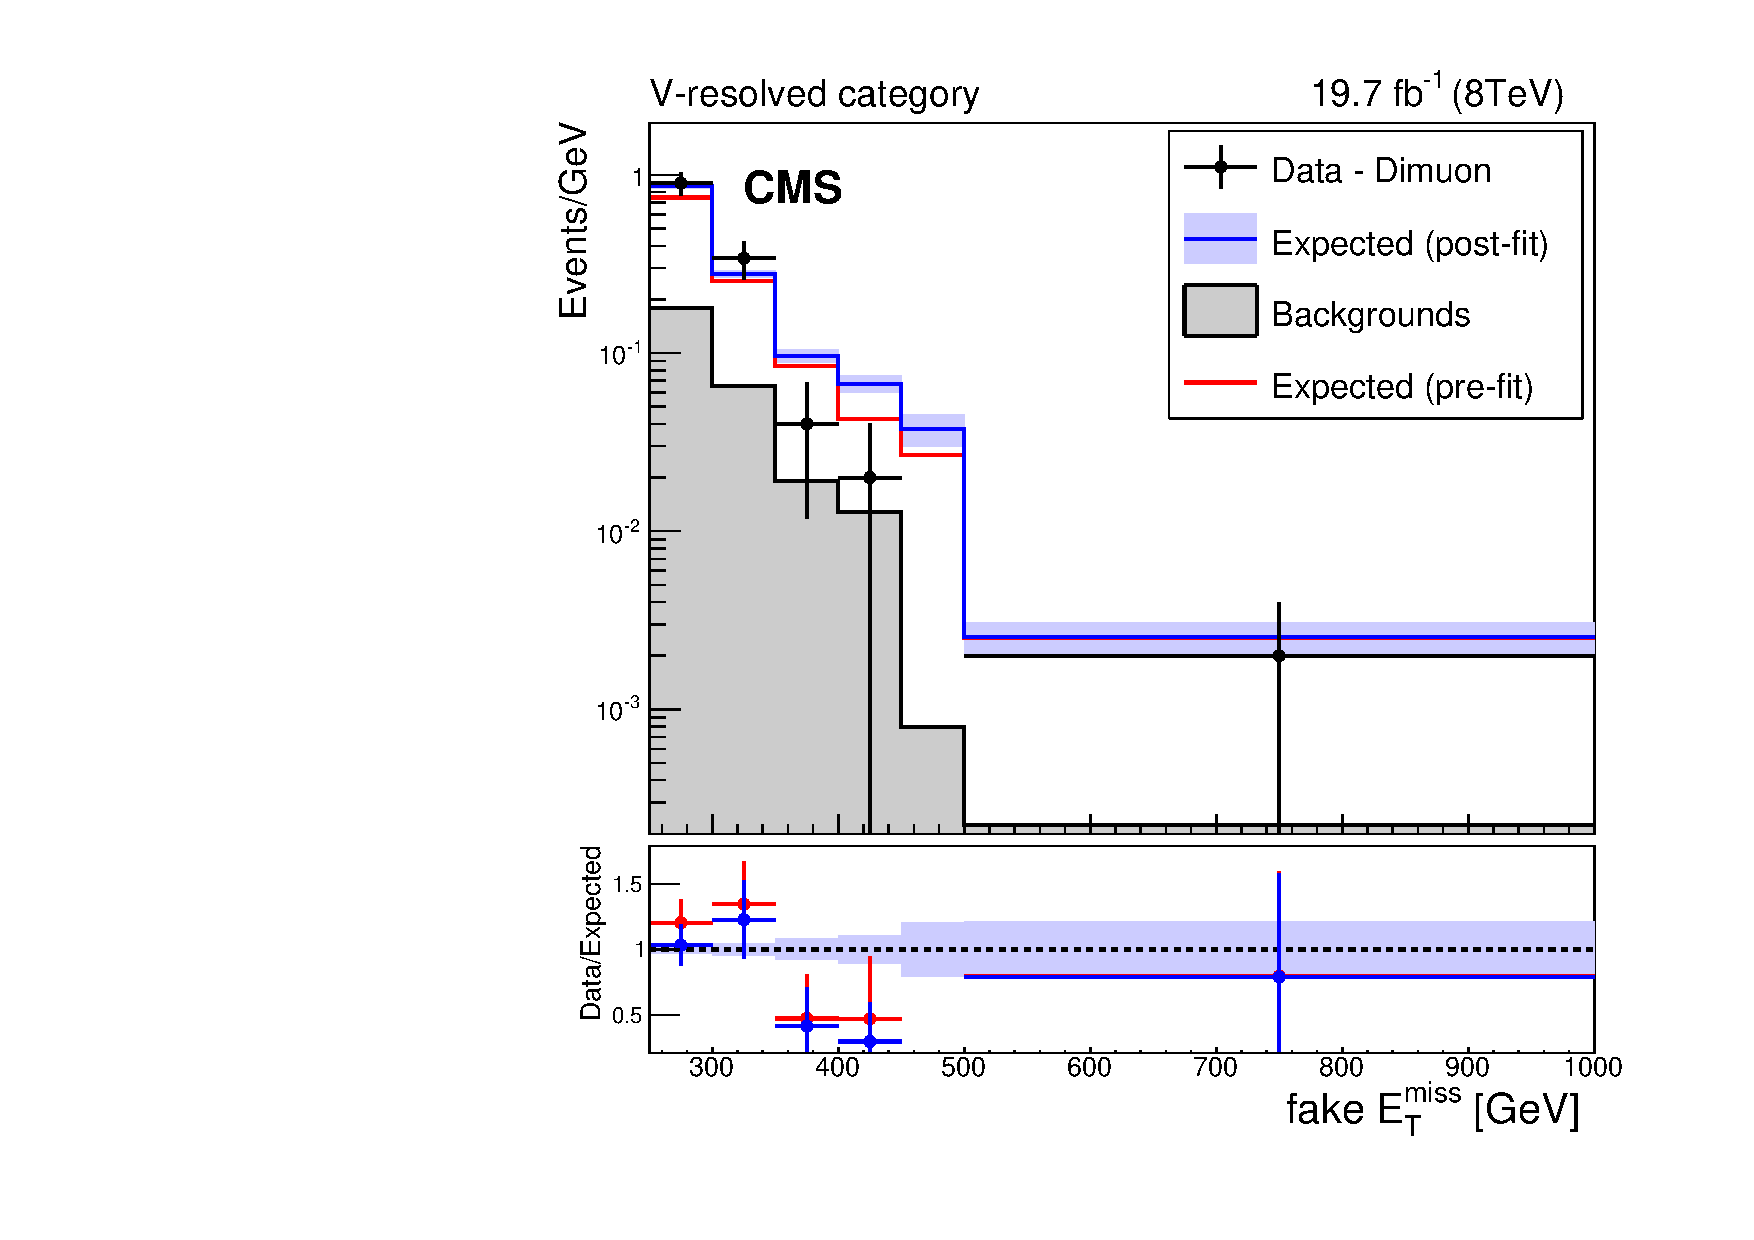
\includegraphics[width=0.32\textwidth]{figures/post_fit_zmm_resolved.pdf}
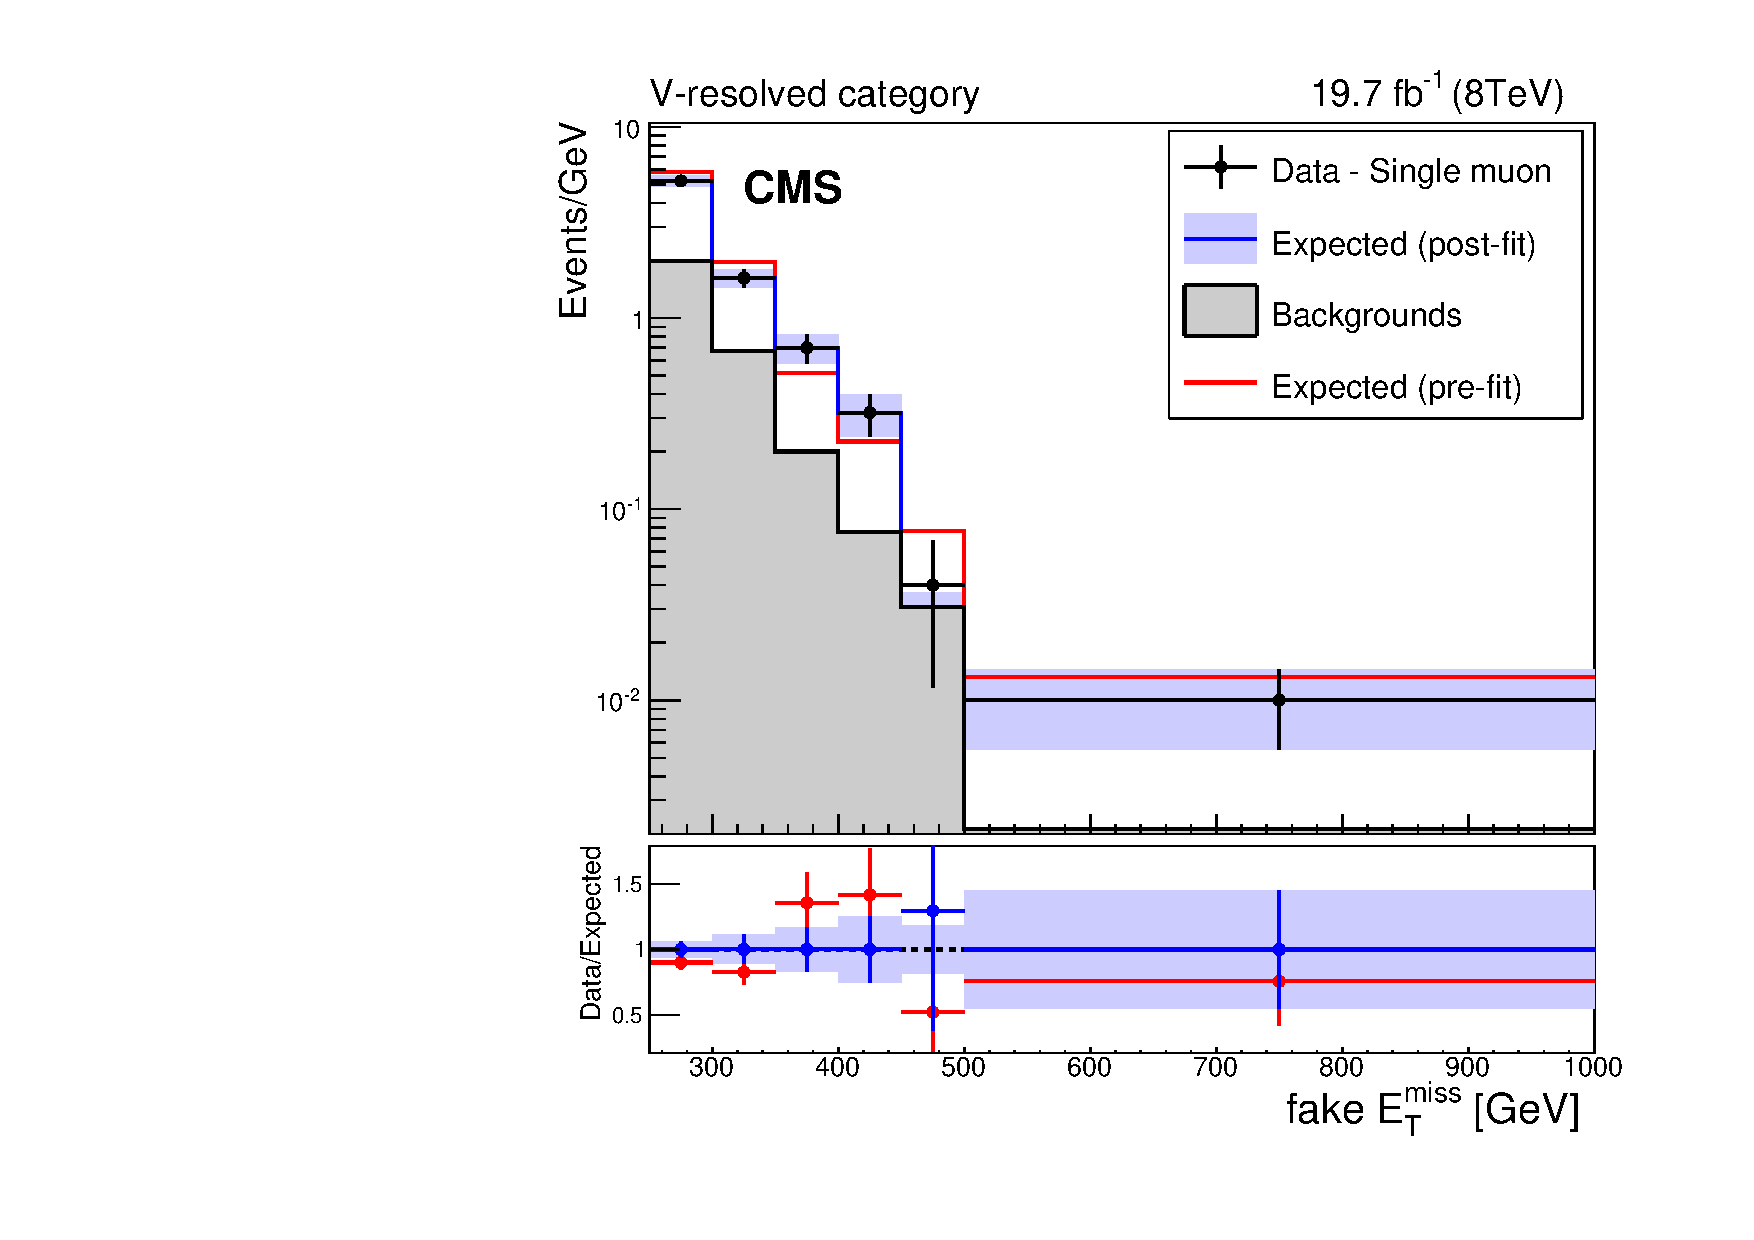
\includegraphics[width=0.32\textwidth]{figures/post_fit_wmn_resolved.pdf}\\
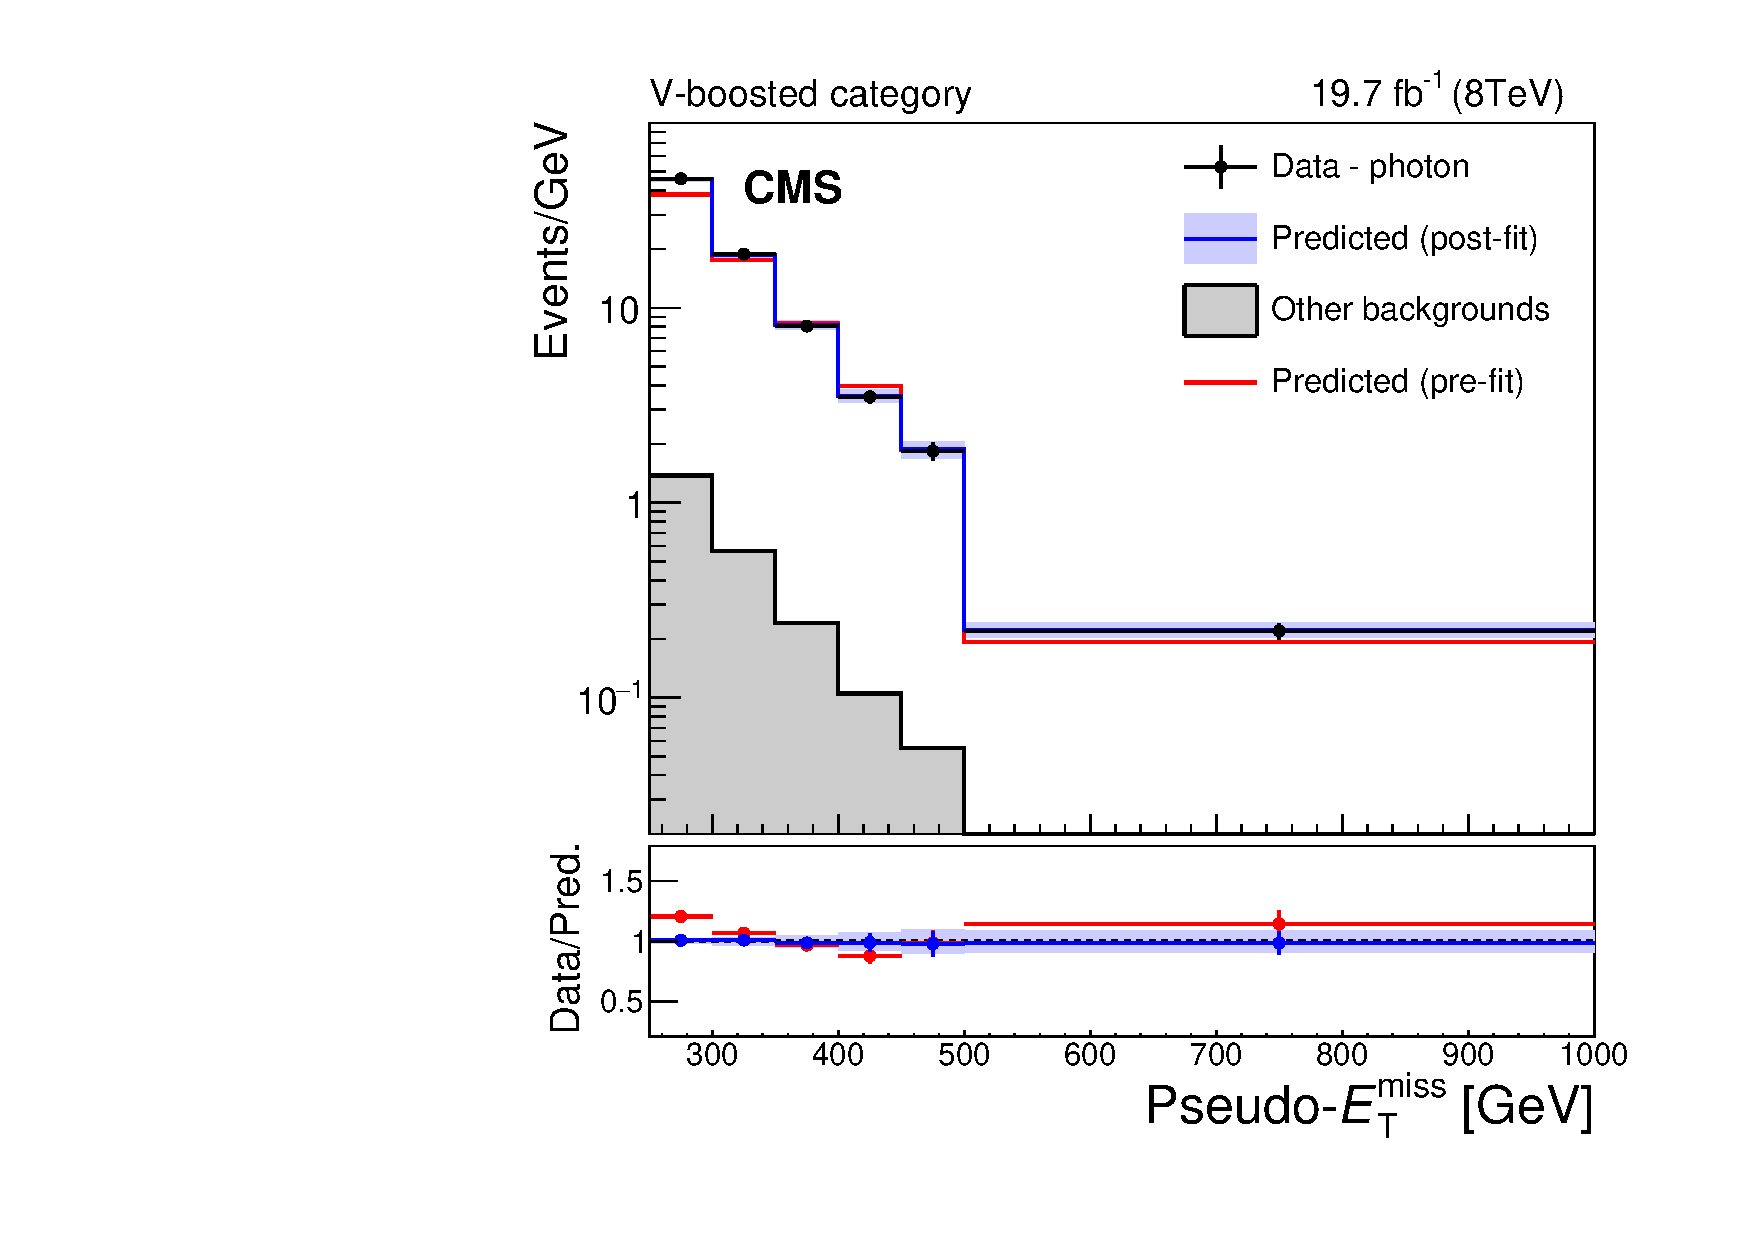
\includegraphics[width=0.32\textwidth]{figures/post_fit_photon_boosted.pdf}
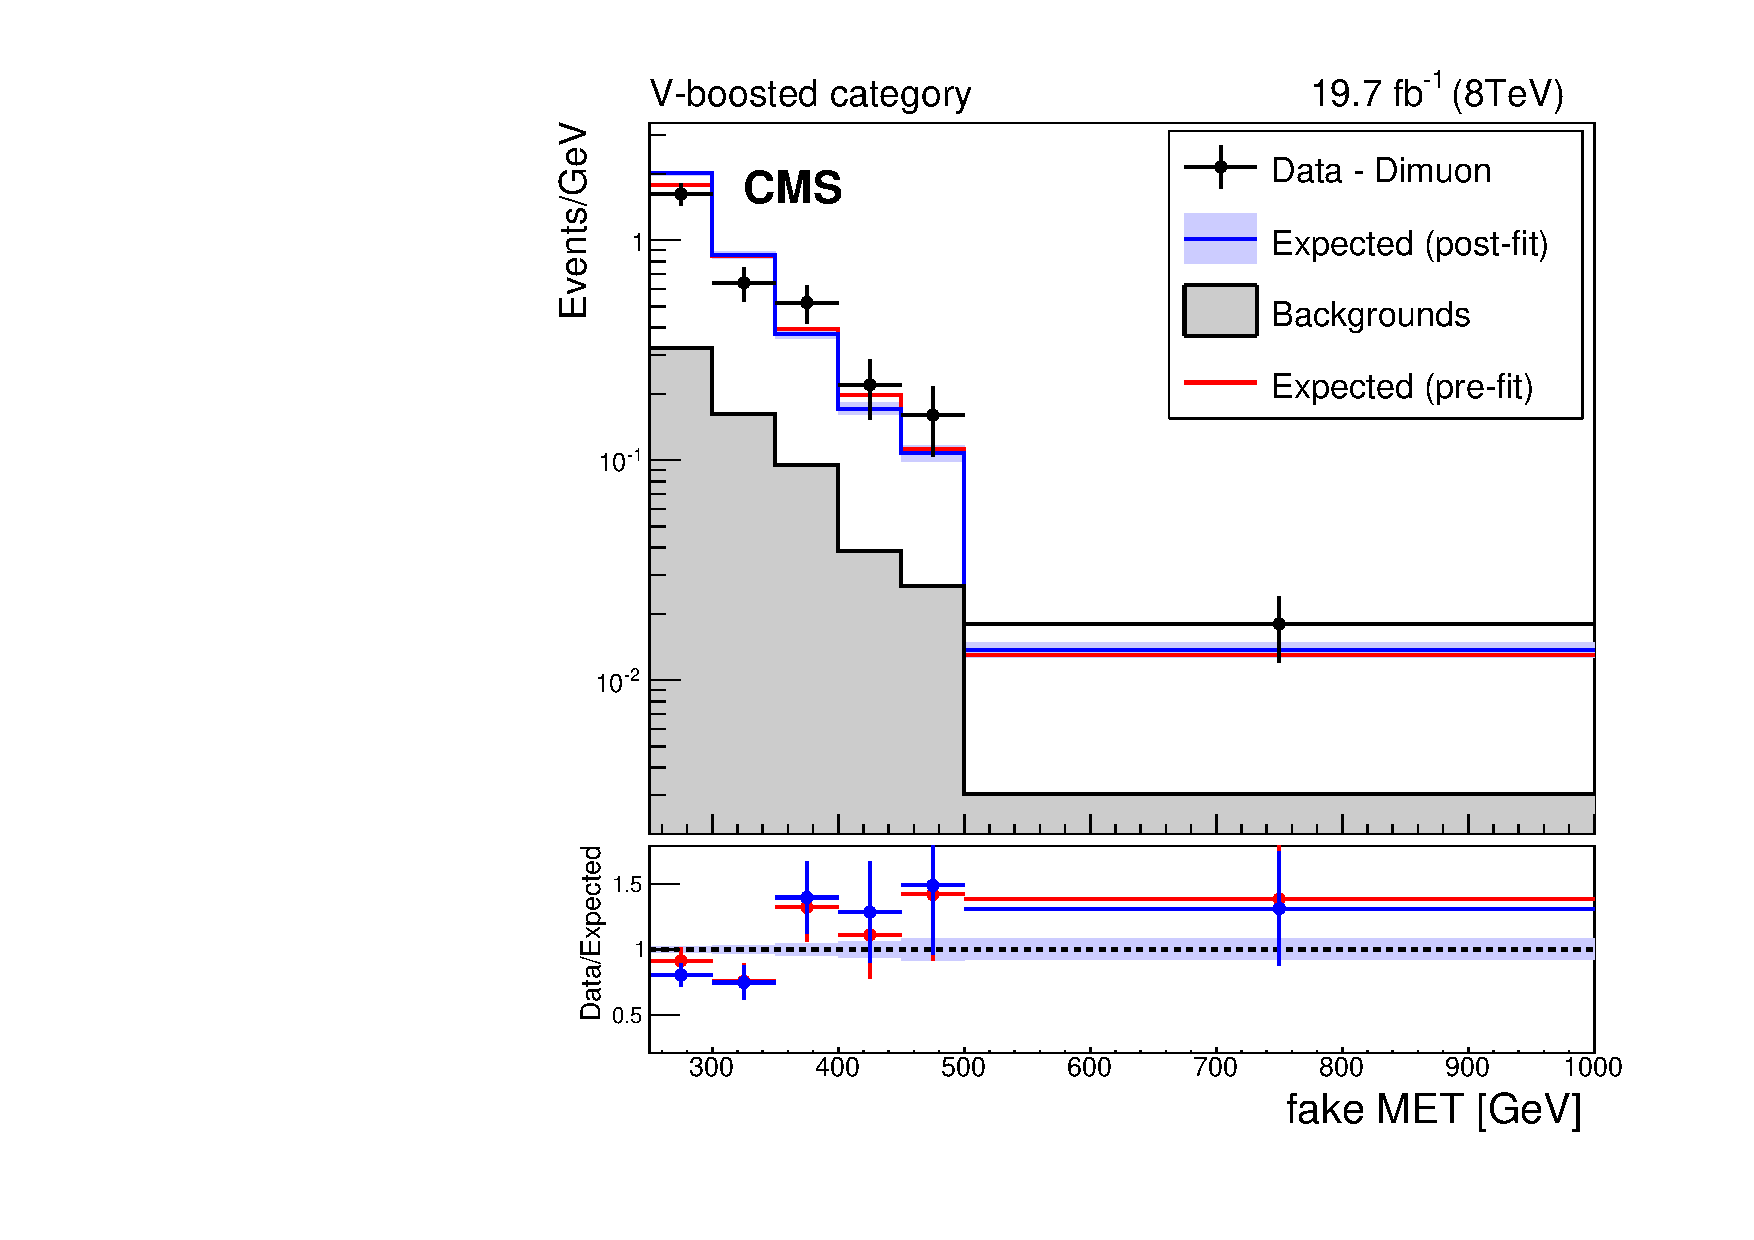
\includegraphics[width=0.32\textwidth]{figures/post_fit_zmm_boosted.pdf}
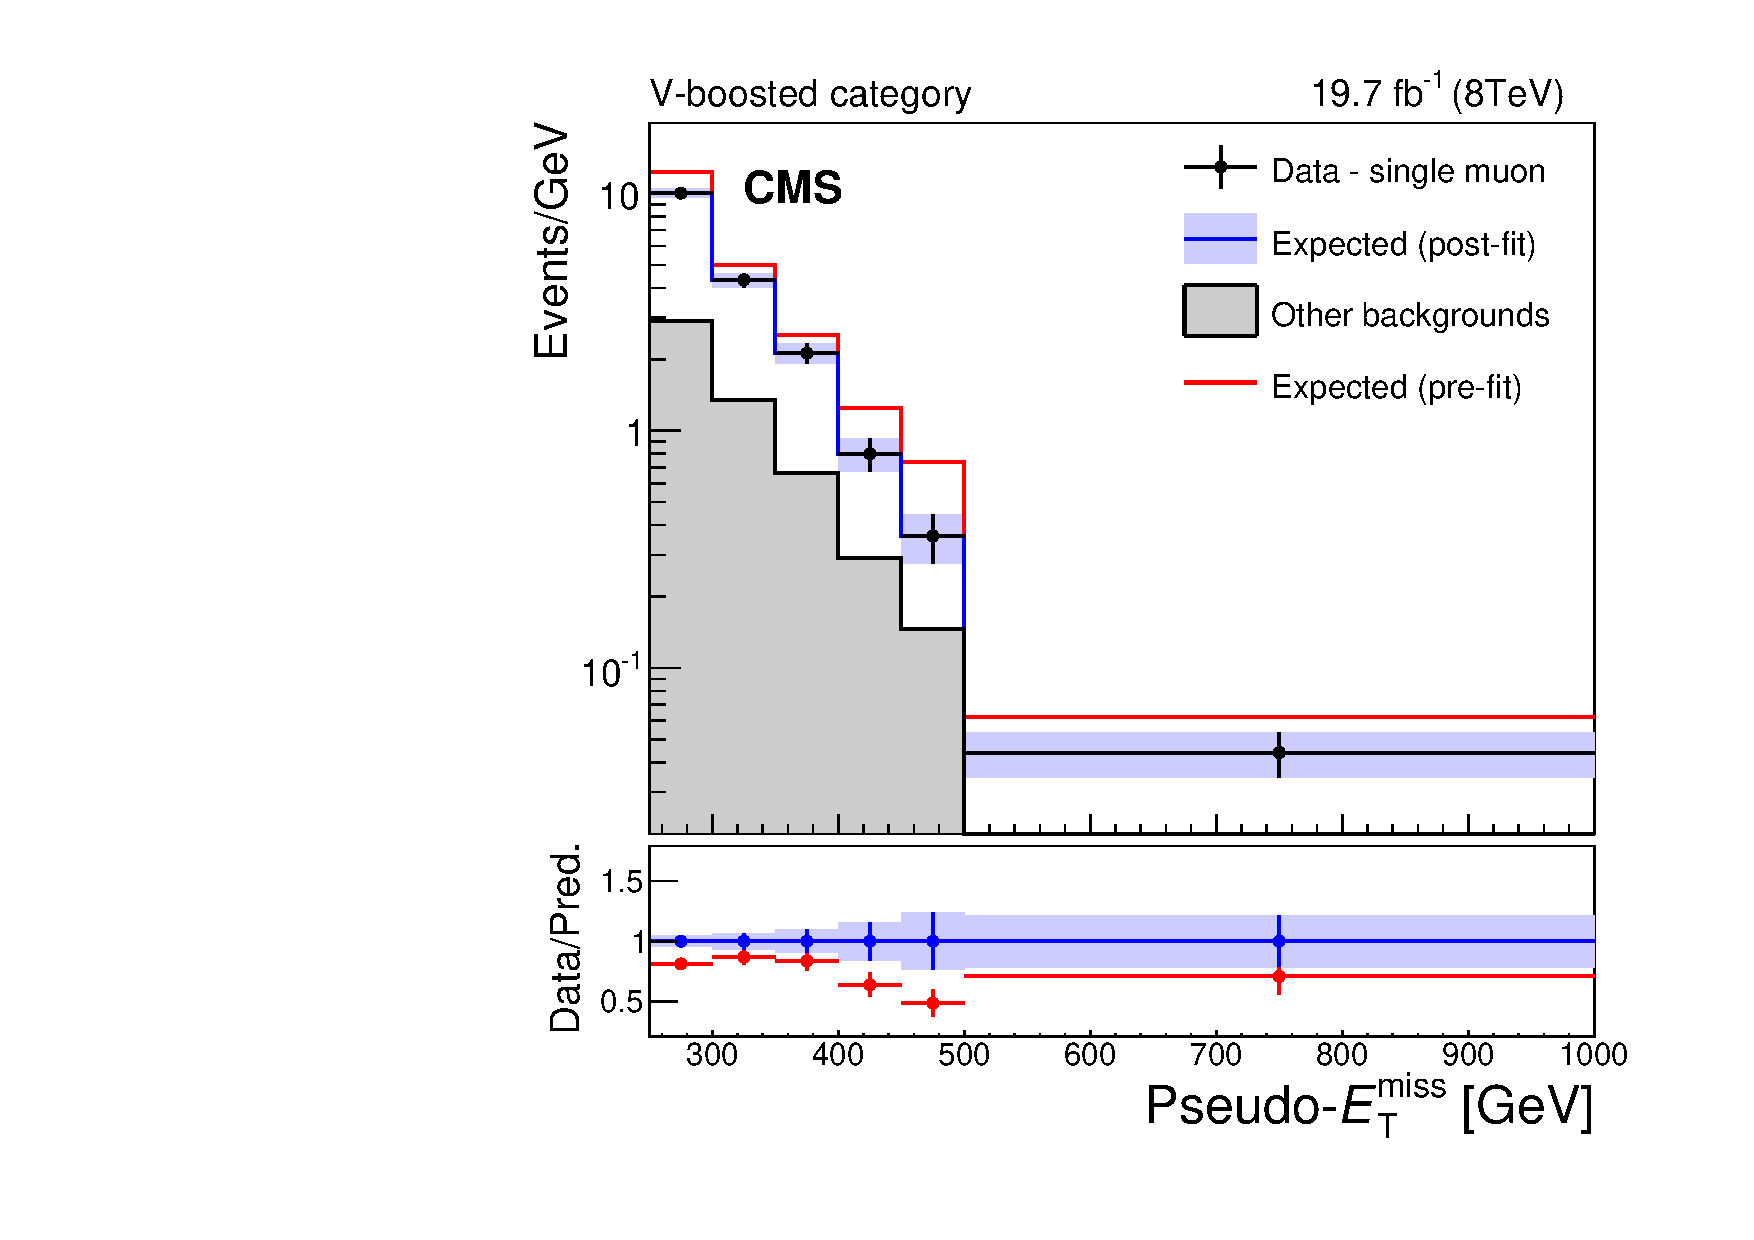
\includegraphics[width=0.32\textwidth]{figures/post_fit_wmn_boosted.pdf}\\
\end{center} \caption{Expected and observed fake \ETm distributions in the
photon~(\cmsLeft), dimuon (middle) and single-muon~(\cmsRight) control regions
after performing the simultaneous likelihood fit to the control regions.  Each
row, from top to bottom, shows the result of the fit in the monojet, V-resolved
and V-boosted event categories, respectively. The red line represents the expected
distribution before fitting the control regions, while the blue line shows
the expectation after the fit. The bottom panels show the ratio of the 
observed data to the expectations pre- and post-fit. The blue bands
indicate the combined statistical and systematic uncertainties from the fit.\label{fig:combined_fit_result} } 
\end{figure}

The remaining backgrounds are expected to be much smaller than those from V$+$jets
and are estimated directly from the simulation.  Shape and normalization
systematic uncertainties from the recoil corrections applied to these
backgrounds are included to account for the uncertainty in the jet energy scale and
resolution. Additionally, a systematic uncertainty of 4\% is included
for the top backgrounds due to the uncertainty of the b-tagging efficiency for
the b-jet veto in the V-resolved category~\cite{CMS-PAS-BTV-13-001}. Systematic uncertainties of 7\% and 10\%
are included for the top~\cite{Khachatryan:2015oqa} and 
diboson~\cite{tagkey2015250,Khachatryan:2015sga}, respectively to account for the uncertainty in their
cross-sections in the releavant kinematic phase-space of this analysis. These individual backgrounds have been studied
separately using dedicated control regions in data in order to validate these
systematic uncertainties. A systematic uncertainty of 50\% is included on the expected 
contribution from  QCD multijet events. This uncertainty was obtained by taking the largest differences 
observed between data and simulation in events selected by inverting the requirement on $\mindphi$.
Finally, a systematic uncertainty of 2.6\% in the
luminosity measurement~\cite{lumi} is included for all of the  
backgrounds derived from simulation.

The expected yields in each bin of \ETm of all SM backgrounds,
after the fit in the control regions, for each of the three signal regions, are given in 
Tables~\ref{tab:bkgmonojet},~\ref{tab:bkgresolved} and~\ref{tab:bkgboosted}. 
The uncertainties represent the sum in quadrature of the effects of all the relevant 
sources of systematic uncertainty in each bin of \ETm. 
The potential correlations of the uncertainties between the different \ETm bins are not 
reflected in these numbers.

\begin{table}[htbp]
  \begin{center}
    \caption{Expected yields of the SM processes and their uncertainties per bin for the monojet category signal region after the fit to the control regions.
      \label{tab:bkgmonojet}}
	\scriptsize
    \begin{tabular}{c|c|c|c|c|c|c|c}
	\hline
	$\ETm$ (GeV) & Obs.  & Z($\rightarrow \nu\nu$)+jets &  W($\rightarrow l\nu$)+jets & Top quark & Dibosons &  Other  & Total Bkg. \\

\hline

      200 - 210 & 17547  &  10742.2$\pm$274.3  &   6771.6$\pm$315.3  &    132.1$\pm$11.3  &    134.5$\pm$13.5  &    539.1$\pm$216.7  &  18332.2$\pm$598.0  \\

      210 - 220 & 14303  &   9234.4$\pm$225.4  &   4988.5$\pm$235.3  &    103.6$\pm$12.5  &    111.5$\pm$11.0  &     58.0$\pm$4.3  &  14500.1$\pm$606.5  \\

      220 - 230 & 11343  &   7316.4$\pm$189.8  &   3832.1$\pm$170.8  &     82.1$\pm$7.3  &     95.1$\pm$9.6  &     44.8$\pm$3.6  &  11371.7$\pm$395.6  \\

      230 - 240 & 8961  &   5727.5$\pm$170.6  &   3019.4$\pm$159.2  &     62.0$\pm$5.8  &     77.9$\pm$8.6  &    111.2$\pm$19.3  &   8942.9$\pm$395.8  \\

      240 - 250 & 6920  &   4678.0$\pm$150.1  &   2470.0$\pm$137.0  &     46.6$\pm$4.4  &     61.0$\pm$6.1  &     78.7$\pm$12.2  &   7293.5$\pm$333.3  \\

      250 - 260 & 5582  &   3702.5$\pm$139.4  &   1858.0$\pm$116.8  &     34.2$\pm$3.7  &     50.1$\pm$4.9  &     48.1$\pm$6.3  &   5670.9$\pm$369.5  \\

      260 - 270 & 4517  &   3287.0$\pm$125.0  &   1579.2$\pm$105.6  &     27.7$\pm$2.3  &     39.7$\pm$4.2  &     11.9$\pm$0.4  &   4949.1$\pm$318.4  \\

      270 - 280 & 3693  &   2567.8$\pm$107.2  &   1101.2$\pm$70.6  &     25.0$\pm$3.1  &     33.5$\pm$3.4  &     23.3$\pm$2.7  &   3741.1$\pm$161.4  \\

      280 - 290 & 2907  &   2085.3$\pm$89.4  &    933.7$\pm$70.9  &     17.8$\pm$1.9  &     28.1$\pm$3.0  &      5.4$\pm$0.1  &   3074.7$\pm$181.5  \\

      290 - 300 & 2406  &   1721.1$\pm$85.2  &    754.1$\pm$58.3  &     15.0$\pm$3.6  &     21.9$\pm$2.7  &     80.7$\pm$10.9  &   2526.6$\pm$170.1  \\

      300 - 310 & 1902  &   1336.6$\pm$78.9  &    577.1$\pm$50.6  &      8.9$\pm$1.6  &     17.7$\pm$2.1  &      3.1$\pm$0.1  &   1945.8$\pm$156.1  \\

      310 - 320 & 1523  &   1181.6$\pm$58.3  &    435.2$\pm$43.2  &      5.9$\pm$2.2  &     15.5$\pm$1.8  &     81.3$\pm$10.3  &   1649.7$\pm$109.6  \\

      320 - 330 & 1316  &    930.7$\pm$53.1  &    370.6$\pm$44.4  &      5.2$\pm$1.3  &     11.0$\pm$1.8  &      2.1$\pm$0.1  &   1321.4$\pm$91.5  \\

      330 - 340 & 1065  &    803.5$\pm$50.9  &    246.0$\pm$28.7  &      4.9$\pm$1.1  &     11.9$\pm$1.8  &      1.8$\pm$0.1  &   1069.7$\pm$116.3  \\

      340 - 360 & 1571  &   1225.2$\pm$60.9  &    398.5$\pm$38.5  &      6.8$\pm$1.2  &     16.4$\pm$1.6  &      5.6$\pm$0.4  &   1652.0$\pm$109.4  \\

      360 - 380 & 1091  &    822.4$\pm$53.3  &    269.1$\pm$30.5  &      3.4$\pm$0.4  &     13.3$\pm$1.4  &      1.3$\pm$0.1  &   1111.4$\pm$148.6  \\

      380 - 420 & 1404  &   1035.9$\pm$65.9  &    324.4$\pm$30.4  &      5.5$\pm$0.6  &     17.1$\pm$1.7  &      1.4$\pm$0.1  &   1387.1$\pm$114.1  \\

      420 - 510 & 1126  &    943.4$\pm$69.7  &    266.9$\pm$26.6  &      3.9$\pm$0.8  &     15.7$\pm$1.6  &     92.7$\pm$9.7  &   1238.9$\pm$139.5  \\

      510 - 1000 & 476  &    330.4$\pm$32.2  &     72.1$\pm$12.2  &      0.6$\pm$0.2  &      8.2$\pm$0.8  &      0.3$\pm$0.1  &    413.0$\pm$71.0  \\

\hline 

    \end{tabular}
  \end{center}
\end{table}


\begin{table}[htbp]
  \begin{center}
    \caption{Expected yields of the SM processes and their uncertainties per bin for the V-resolved category signal region after the fit to the control regions.
      \label{tab:bkgresolved}}
	\scriptsize
    \begin{tabular}{l|c|c|c|c|c|c|c}
	\hline
	$\ETm$ (GeV) & Obs.  & Z($\rightarrow \nu\nu$)+jets &  W($\rightarrow l\nu$)+jets & Top quark & Dibosons &  Other  & Total Bkg. \\
\hline

      250 - 300 & 617  &    298.0$\pm$35.8  &    166.0$\pm$26.4  &     55.4$\pm$4.7  &     27.9$\pm$1.6  &     39.2$\pm$16.9  &    587.1$\pm$48.3  \\

      300 - 350 & 211  &     97.8$\pm$13.9  &     40.7$\pm$10.4  &     15.2$\pm$1.5  &      9.6$\pm$0.3  &     12.3$\pm$3.8  &    170.0$\pm$17.7  \\

      350 - 400 & 79  &     31.1$\pm$7.0  &     21.5$\pm$8.9  &      5.5$\pm$0.7  &      3.2$\pm$0.3  &      2.0$\pm$0.4  &     62.1$\pm$11.7  \\

      400 - 450 & 20  &     20.1$\pm$6.4  &     14.5$\pm$8.5  &      1.5$\pm$0.2  &      0.6$\pm$0.3  &      6.3$\pm$1.4  &     38.3$\pm$10.5  \\

      450 - 500 & 16  &      6.1$\pm$2.7  &      1.0$\pm$2.6  &      1.0$\pm$0.4  &      0.4$\pm$0.1   & -  &      8.5$\pm$3.6  \\

      500 - 1000 & 17  &      6.9$\pm$3.0  &      2.6$\pm$1.7  &      0.3$\pm$0.2  &      0.5$\pm$0.0  &      7.6$\pm$1.4  &     11.6$\pm$3.5  \\

\hline 
    \end{tabular}
\bigskip
\bigskip
\bigskip
    \caption{Expected yields of the SM processes and their uncertainties per bin for the V-boosted category signal region after the fit to the control regions.
      \label{tab:bkgboosted}}
	\scriptsize
    \begin{tabular}{l|c|c|c|c|c|c|c}
	\hline
	$\ETm$ (GeV) & Obs.  & Z($\rightarrow \nu\nu$)+jets &  W($\rightarrow l\nu$)+jets & Top quark & Dibosons &  Other  & Total Bkg. \\
\hline 

      250 - 300 & 1073  &    682.5$\pm$40.1  &    278.8$\pm$32.5  &     35.4$\pm$3.7  &    103.2$\pm$14.6  &      2.5$\pm$0.1  &   1103.0$\pm$63.4  \\

      300 - 350 & 453  &    271.4$\pm$22.8  &    114.3$\pm$19.6  &     12.7$\pm$1.3  &     46.5$\pm$6.9  &      0.7$\pm$0.1  &    445.7$\pm$33.9  \\

      350 - 400 & 160  &    117.4$\pm$12.8  &     38.3$\pm$8.7  &      5.6$\pm$1.0  &     22.2$\pm$3.3  &      0.2$\pm$0.1  &    184.0$\pm$18.1  \\

      400 - 450 & 81  &     49.7$\pm$7.3  &      9.8$\pm$3.4  &      1.5$\pm$0.8  &     11.0$\pm$1.8   & -  &     72.1$\pm$28.9  \\

      450 - 500 & 30  &     31.2$\pm$6.1  &      5.0$\pm$2.6  &      0.5$\pm$0.1  &      7.4$\pm$1.1   & -  &     44.3$\pm$6.6  \\

      500 - 1000 & 39  &     39.8$\pm$7.8  &      6.4$\pm$3.4  &      0.2$\pm$0.0  &      7.8$\pm$1.1   & -  &     54.3$\pm$8.5  \\

\hline 
    \end{tabular}
  \end{center}
\end{table}

\begin{section}{Results}

A simultaneous fit is performed to the signal region across the three event categories,
allowing for systematic uncertainties in the background expectations. 
The corresponding comparisons between data and background in the
\ETm distributions, for each of the three categories, after this fit are shown
in Fig.~\ref{fig:post_fit_plots}.   Agreement between the expected SM
backgrounds and data is observed at the percent level across the three
categories. A local significance of the data in each bin is calculated by
comparing the likelihood between the background-only fit  
(Fig.~\ref{fig:post_fit_plots}) and another fit, setting the expected total yield of
events in that bin to the observation in data. The largest local significance
observed using this procedure is $1.9$ standard deviations and corresponds to the largest \ETm
bin of the monojet category.


\begin{figure*}[hbtp]\begin{center} \subfloat[][]{
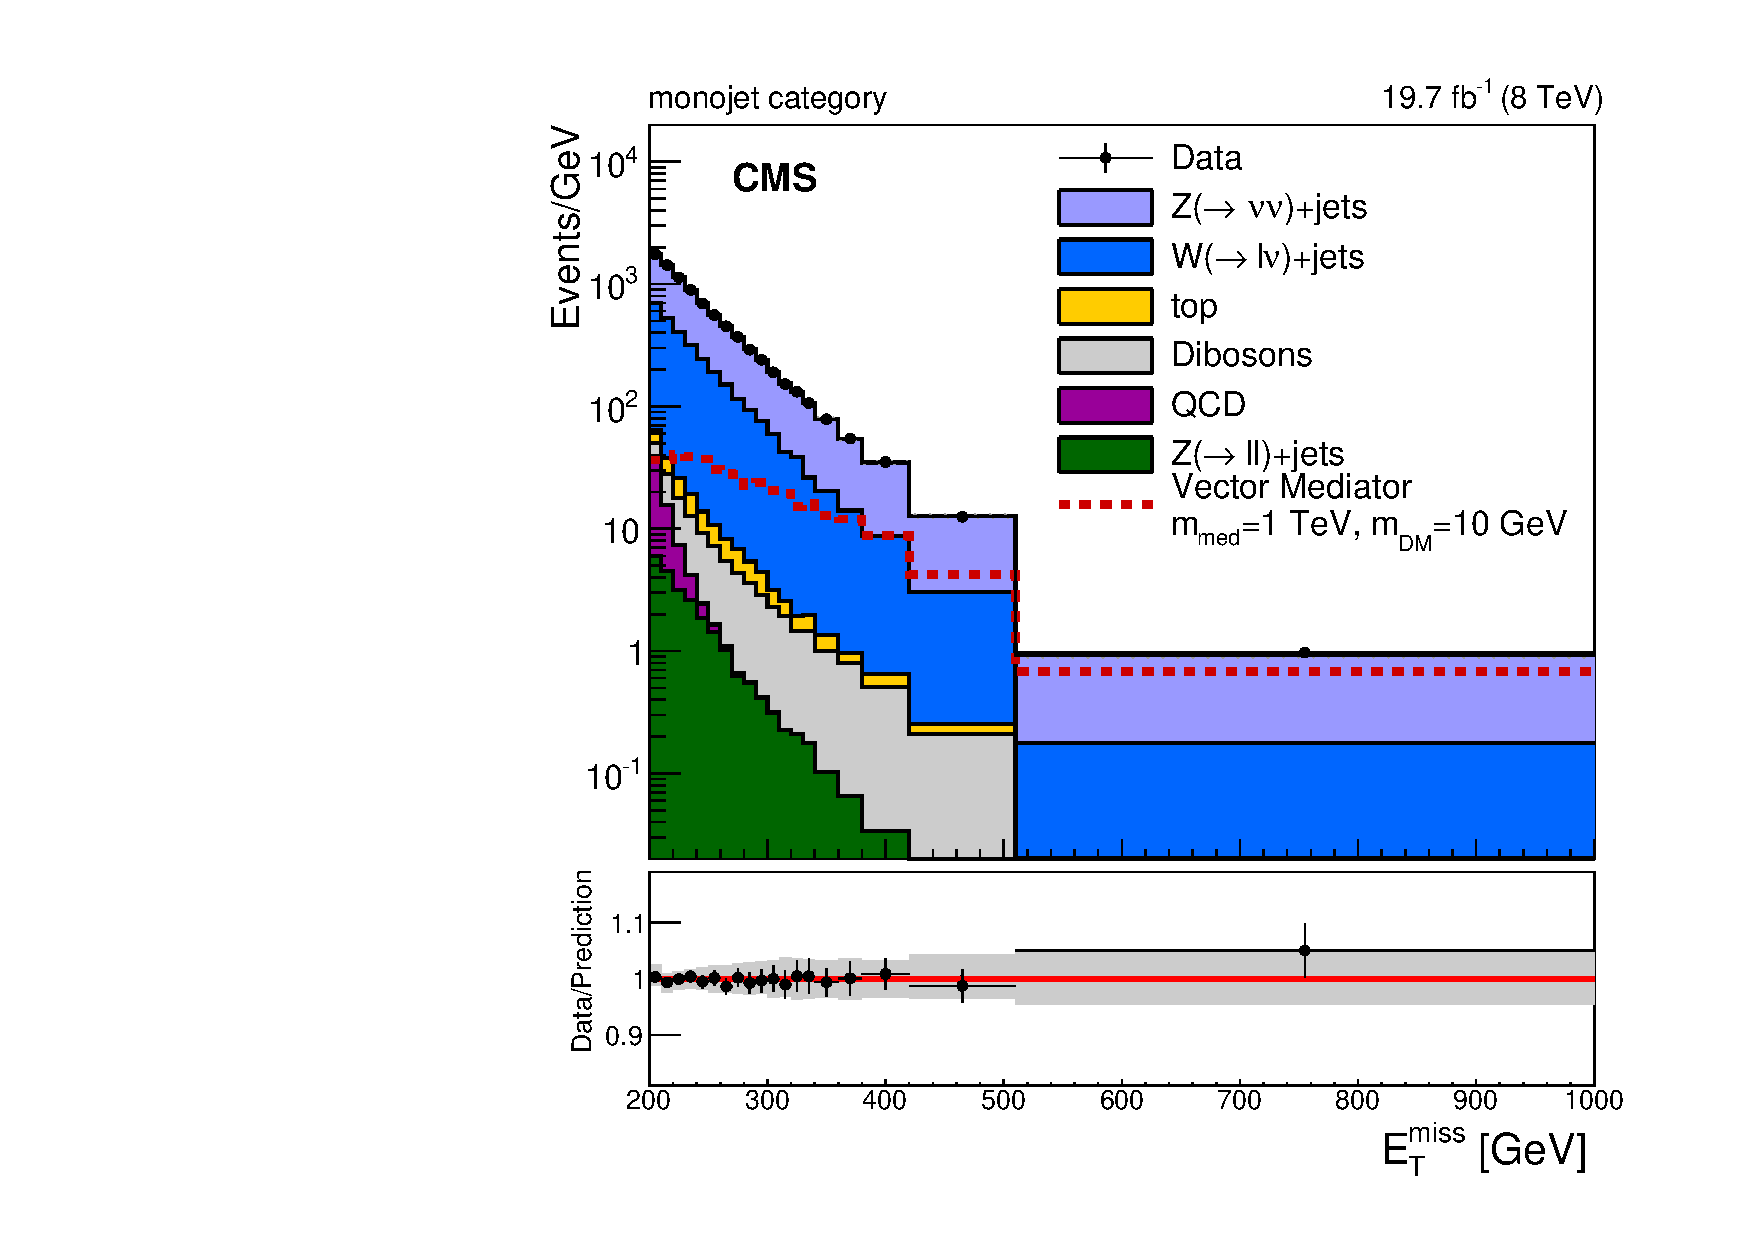
\includegraphics[width=0.5\textwidth]{figures/plot_config_monojet.pdf} }
\subfloat[][]{
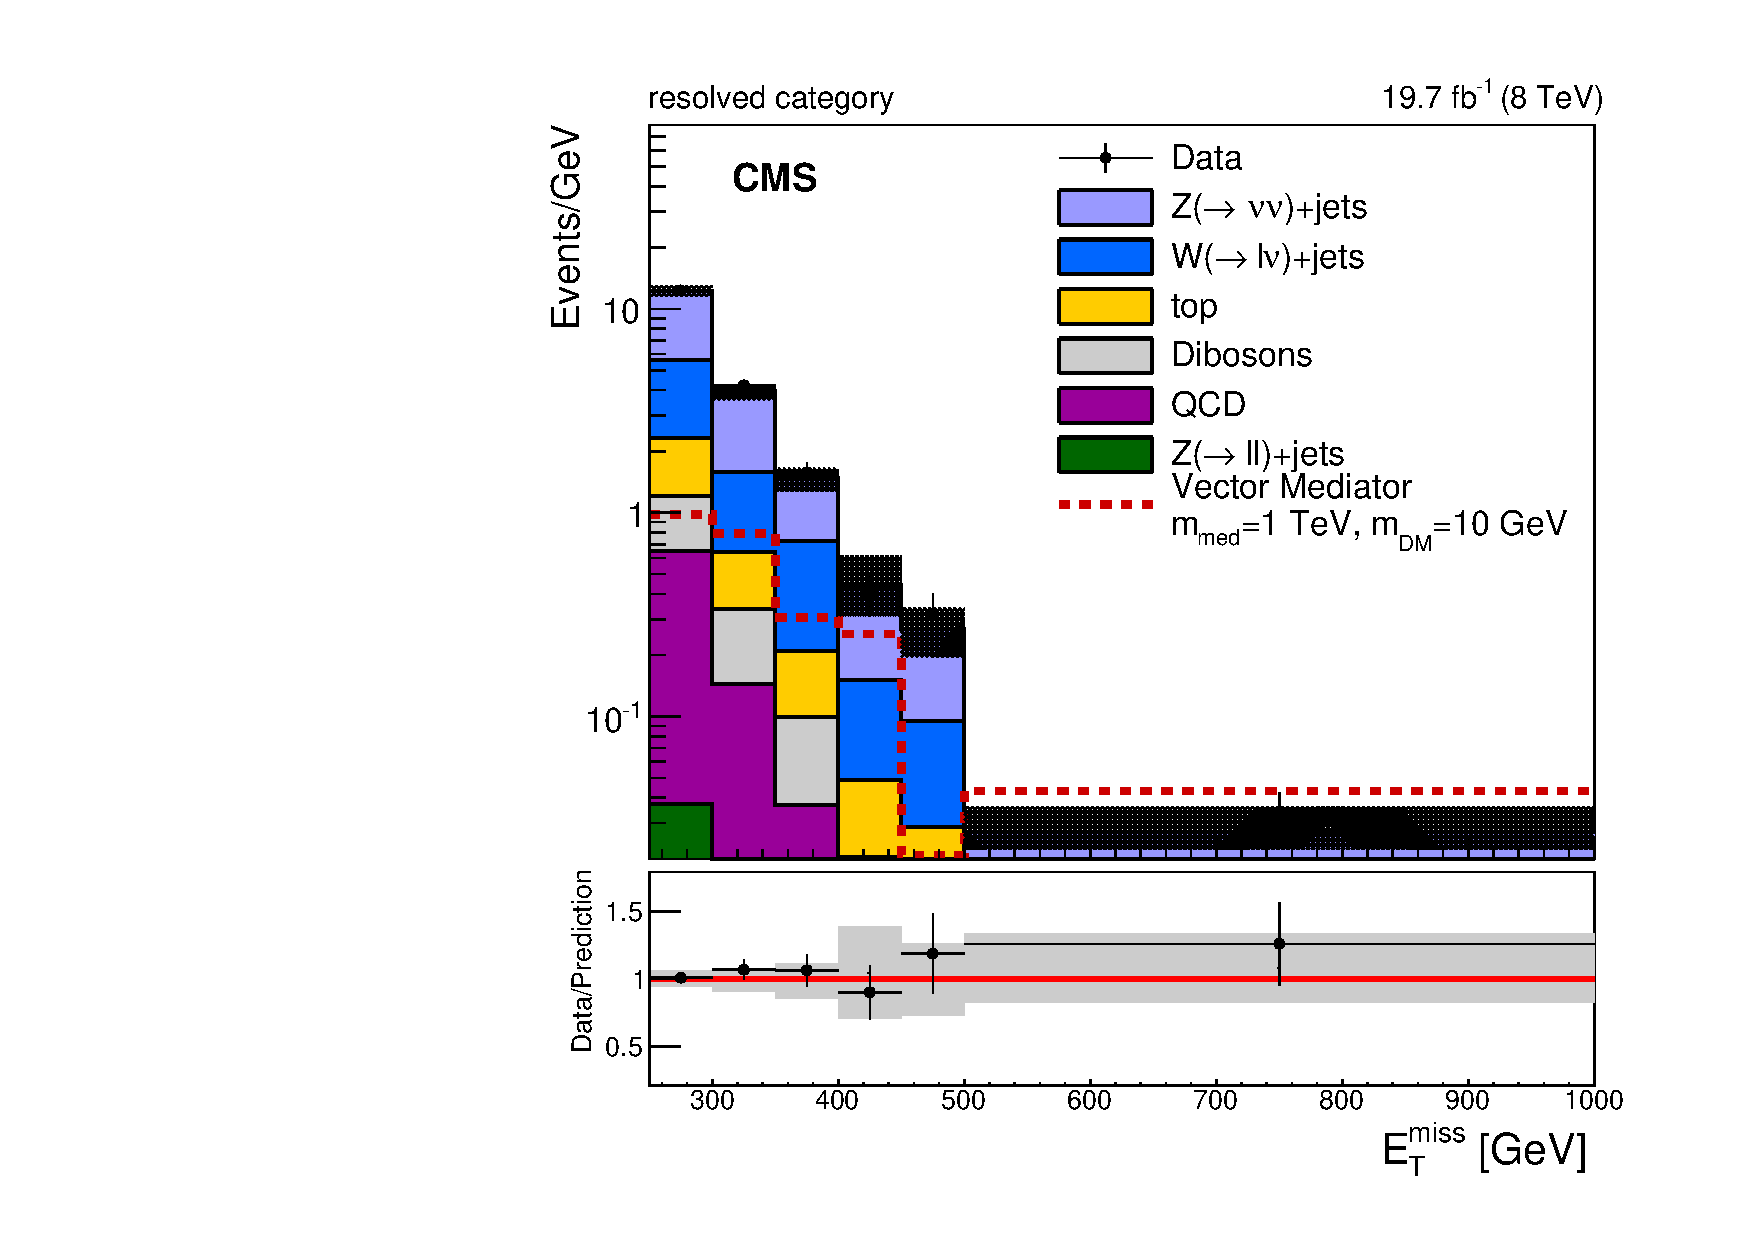
\includegraphics[width=0.5\textwidth]{figures/plot_config_resolved.pdf} }\\
\subfloat[][]{
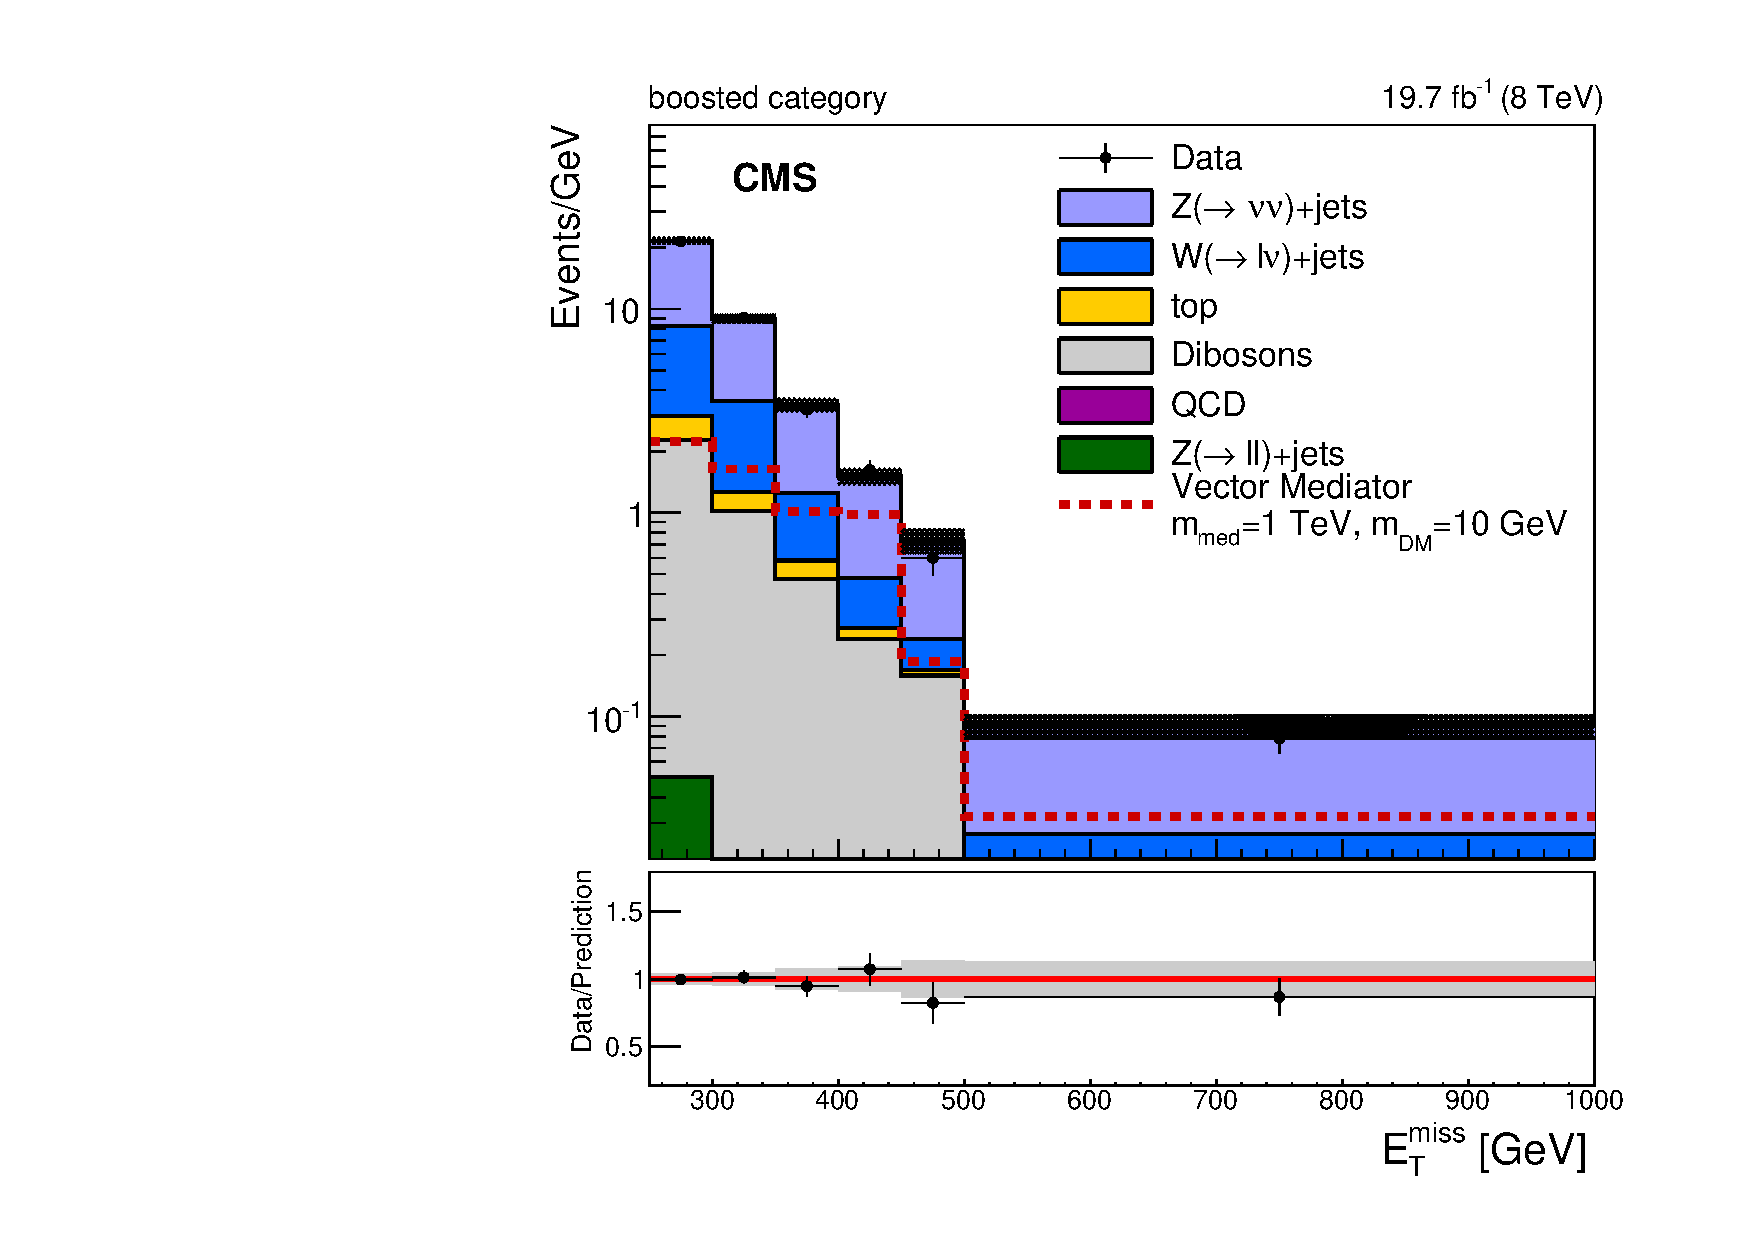
\includegraphics[width=0.5\textwidth]{figures/plot_config_boosted.pdf} }
\caption{ Post-fit distributions of \ETm expected from SM backgrounds and
observed in data in the signal region. The expected distributions are evaluated
after fitting to the observed data simultaneously across the (a) monojet, 
(b) V-resolved and (c) V-boosted categories.  The gray bands indicate the post-fit
uncertainty on the background, assuming no signal. The expected distribution
assuming vector mediated DM production is shown for $m_{\mathrm{DM}}=10$\GeV and 
$m_{\mathrm{MED}} = 1 $ TeV.  } \label{fig:post_fit_plots}\end{center}\end{figure*}

Exclusion limits are set for these models using the asymptotic CLs method~\cite{CMS-NOTE-2011-005,cls} with a
profile likelihood ratio as the test statistic in which systematic uncertainties
are modelled as nuisance parameters.  For each signal hypothesis tested, upper
limits are placed on the ratio of the signal cross section to the predicted
cross-section, denoted as $\mu=\sigma/\sigma_{\mathrm{TH}}$. Limits are presented in
terms of excluded regions in the $m_{\mathrm{MED}}--m_{\textrm{DM}}$ plane,
assuming scalar, pseudoscalar, vector, and axial-vector mediators, and
determining the points for which $\mu\ge1$ is excluded at the 90\% confidence level 
(CL) or more. The choice 
of determining 90\% CL is to allow for comparison with other experiments. 
Experimental systematic uncertainties, including jet and \ETm response and
resolution, are included in the signal model as nuisance parameters, while the
theoretical systematic uncertainties on the inclusive cross section (20\% and
30\% for the vector and axial vector, and scalar and pseudoscalar models,
respectively) due to QCD scale and PDF uncertainties are instead added as
additional contours to the exclusion limits. These uncertainties are chosen to
be conservative across the full range of the mediator mass from 10~\GeV to 3~\TeV.

%To compare direct detection experiments with collider experiments, the direct
%detection bounds can be interpreted under the Lagrangians given in
%Eq.~\ref{eq:LS}. The limits obtained in the simplified models use the
%standard approaches to compute $t$-channel
%scattering~\cite{Kurylov:2003ra,Hisano:2010ct,
%Cheung:2013pfa,Buchmueller:2014yoa}.  


Figure~\ref{fig:masslims} shows the 90\% CL exclusions for the vector,
axial vector, scalar and pseudoscalar mediator models.  The expected 90\% confidence
level upper limit on the ratio of excluded cross section to the predicted
cross-section ($\mu_{\textrm{up}}$), when assuming the mediator only couples to
fermions (fermionic), is shown by the blue color scale. The limits are calculated under
the minimum width constraint~\cite{An:2012va,Abercrombie:2015wmb,Fox:2011pm,simplified1}. 
For the pseudoscalar interpretation, there is a region of  
masses between 150 and 280\GeV for which the decrease in 
cross-section with larger mediator mass is balanced by an increase in acceptance for the 

%To compare limits from direct detection experiments with those
%obtained here, the DD bounds can be interpreted under the Lagrangians given by
%Eq.~\ref{eq:LS}-Eq.~\ref{eq:LA}. The limits obtained in the simplified models use the
%standard approaches to compute $t$-channel
%scattering~\cite{Kurylov:2003ra,Hisano:2010ct,
%Cheung:2013pfa,Buchmueller:2014yoa}.  For the vector and scalar  models,
%the limits are compared with the measurements by the
%LUX collaboration~\cite{Akerib:2012ys}, which currently
%provide the strongest constraints for $m_{\rm{DM}} \gtrsim 4$ GeV~\cite{PhysRevLett.116.161301}. 
%For axial vector couplings, the limits are compared with DM-proton scattering limits
%from PICO-2 collaborationL~\cite{Amole:2015lsj}.  For pseudoscalar interactions, direct
%detection bounds are strongly velocity suppressed.  The most appropriate
%comparison is therefore to the most sensitive bounds from indirect detection
%from FermiLAT collaboration~\cite{Ackermann:2011wa,Abdo:2010ex}.  These limits apply to the
%scenario in which DM is annihilated in the center of a galaxy, producing
%a $\gamma$ ray signature.  The results are also compared, for all four types of
%mediators, to constraints obtained from the observed cosmological relic density
%of DM as determined from measurements of the cosmic microwave background by the
%WMAP and Planck experiments~\cite{Bennett:2003ba,Planck:2006aa}. The expected DM
%abundance is estimated, separately for each model, using a thermal freeze-out
%mechanism implemented in {\sc MadDM 1.0}~\cite{Backovic:2013dpa}, and compared to the
%observed cold DM density $\Omega_c h^2=0.12$~\cite{Ade:2013zuv}, as described in 
%Ref.~\cite{Pree:2016hwc}. It is assumed that the simplified model hypothesised 
%provides the only relevant beyond SM dynamics for DM interactions.

signal so that the expected signal contribution remains roughly constant. The expected 
value of $\mu_{\mathrm{up}}$ is larger than 1 for this region resulting in an  
island at low dark matter masses. No exclusion is expected at the 90\% CL therefore in this region. 
However, the observed value of $\mu_{\mathrm{up}}$ is smaller than 1 throughout this 
The results are compared, for all four types of
mediators, to constraints obtained from the observed cosmological relic density
of DM as determined from measurements of the cosmic microwave background by the
WMAP and Planck experiments~\cite{Bennett:2003ba,Planck:2006aa}. The expected DM
abundance is estimated, separately for each model, using a thermal freeze-out
mechanism implemented in {\sc MadDM}~\cite{Backovic:2013dpa}, and compared to the
observed cold DM density $\Omega_c h^2=0.12$~\cite{Ade:2013zuv} as described in 
Ref.~\cite{Pree:2016hwc}. It is assumed that the simplified model hypothesised 
provides the only relevant beyond SM dynamics for DM interactions.
egion at 90\% CL so no such island appears in the observed limits. 

%Under the vector mediator model, the DD bounds dominate across
%most of the plane, while for the axial vector, there is good complementarity
%between the DD limits and those from this analysis as shown in Fig.~\ref{fig:masslims}(b). 
%Limits in the scalar mediator scenario are more sensitive than those
%from DD experiments for small DM masses as shown in Fig.~\ref{fig:masslims}(c). Additional sensitivity is gained for mediator
%masses greater than 350 \GeV, due to the rise in cross section of the
%gluon fusion loop process for masses greater than twice the top quark mass. In
%the pseudoscalar mediator scenario, the limits from this analysis exceed the
%reach in $m_{\mathrm{MED}}$ beyond those from FermiLAT over the whole region.

\begin{figure}[htbp] \centering \subfloat[][]{
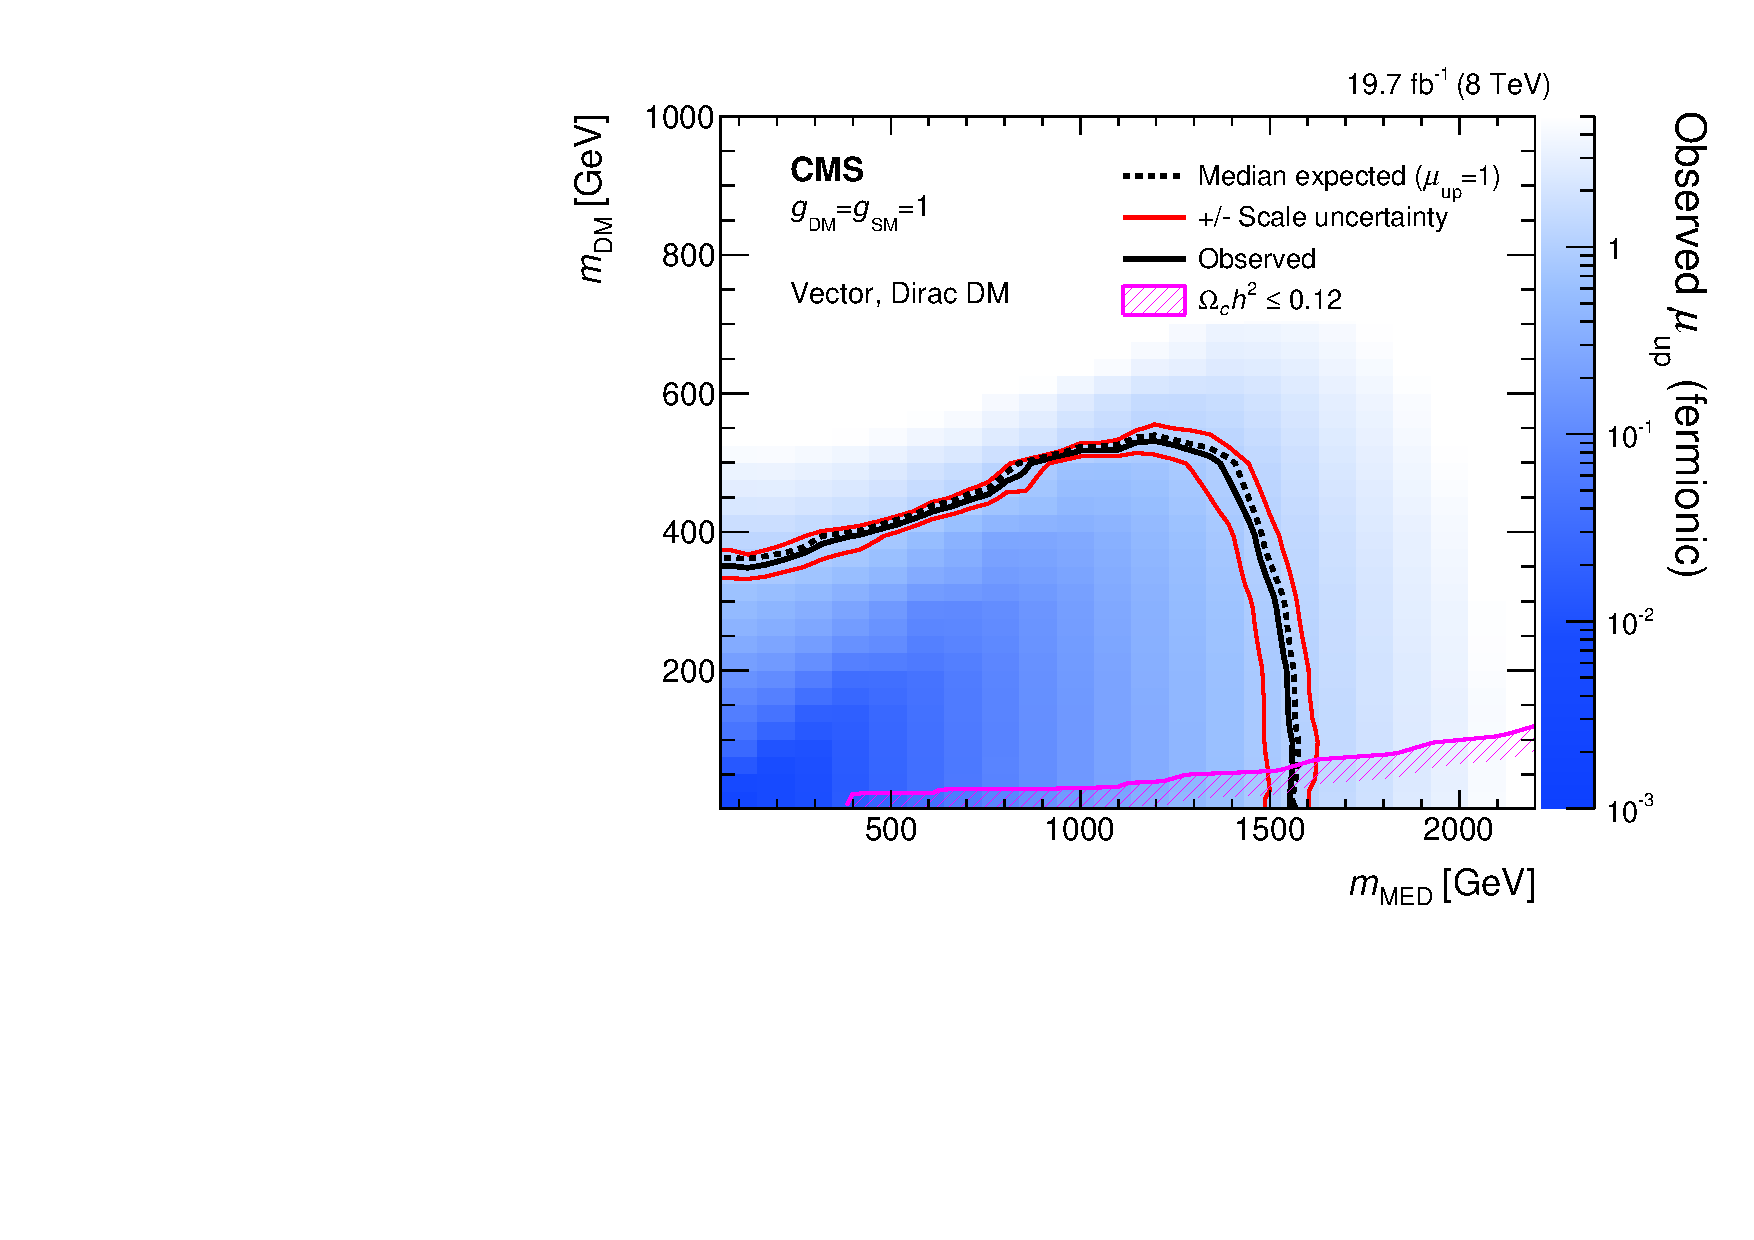
\includegraphics[angle=0,width=0.50\textwidth]{figures/MassLimit_1_800_0_Both.pdf}
\label{fig:mass_800} } \subfloat[][]{
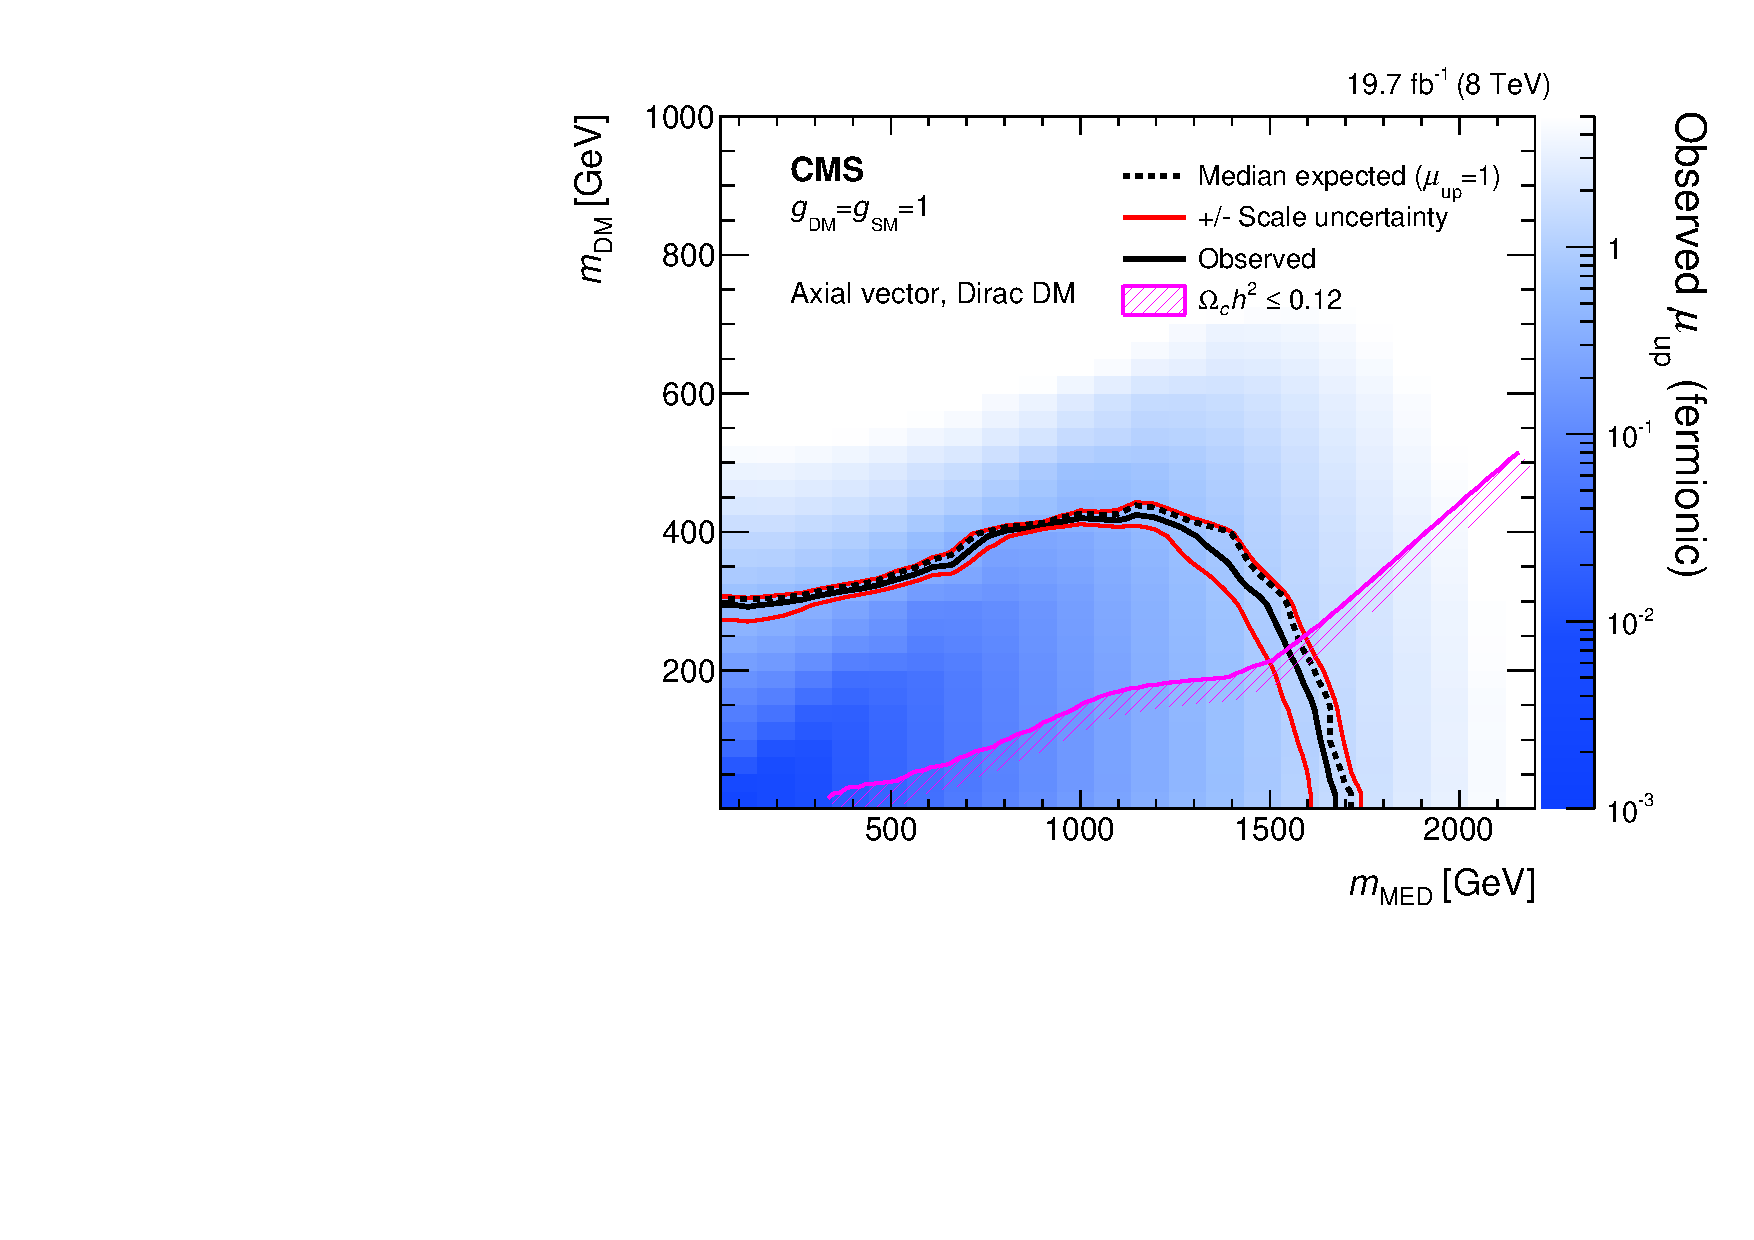
\includegraphics[angle=0,width=0.50\textwidth]{figures/MassLimit_1_801_0_Both.pdf}
\label{fig:mass_801} }\\ \subfloat[][]{
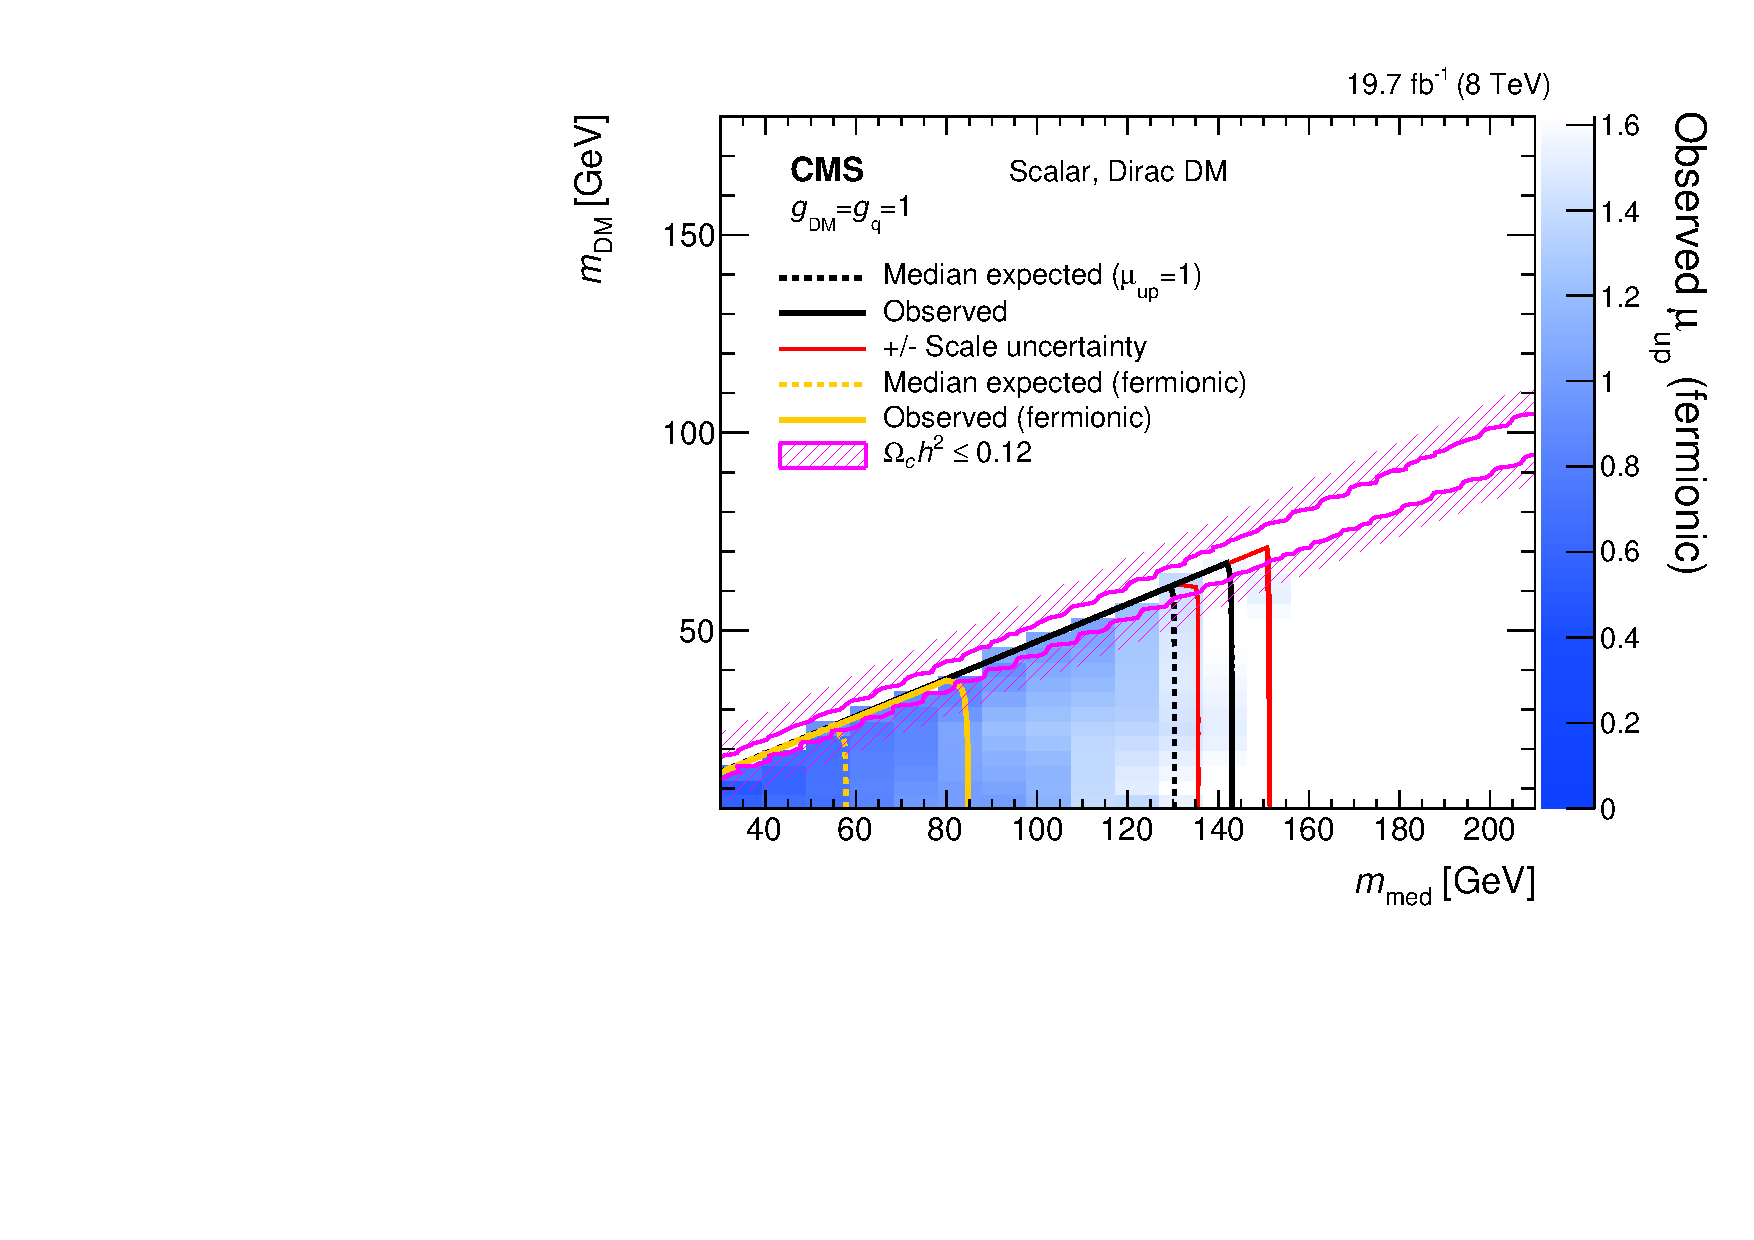
\includegraphics[angle=0,width=0.50\textwidth]{figures/MassLimit_1_805_0_Both.pdf}
\label{fig:mass_805} } \subfloat[][]{
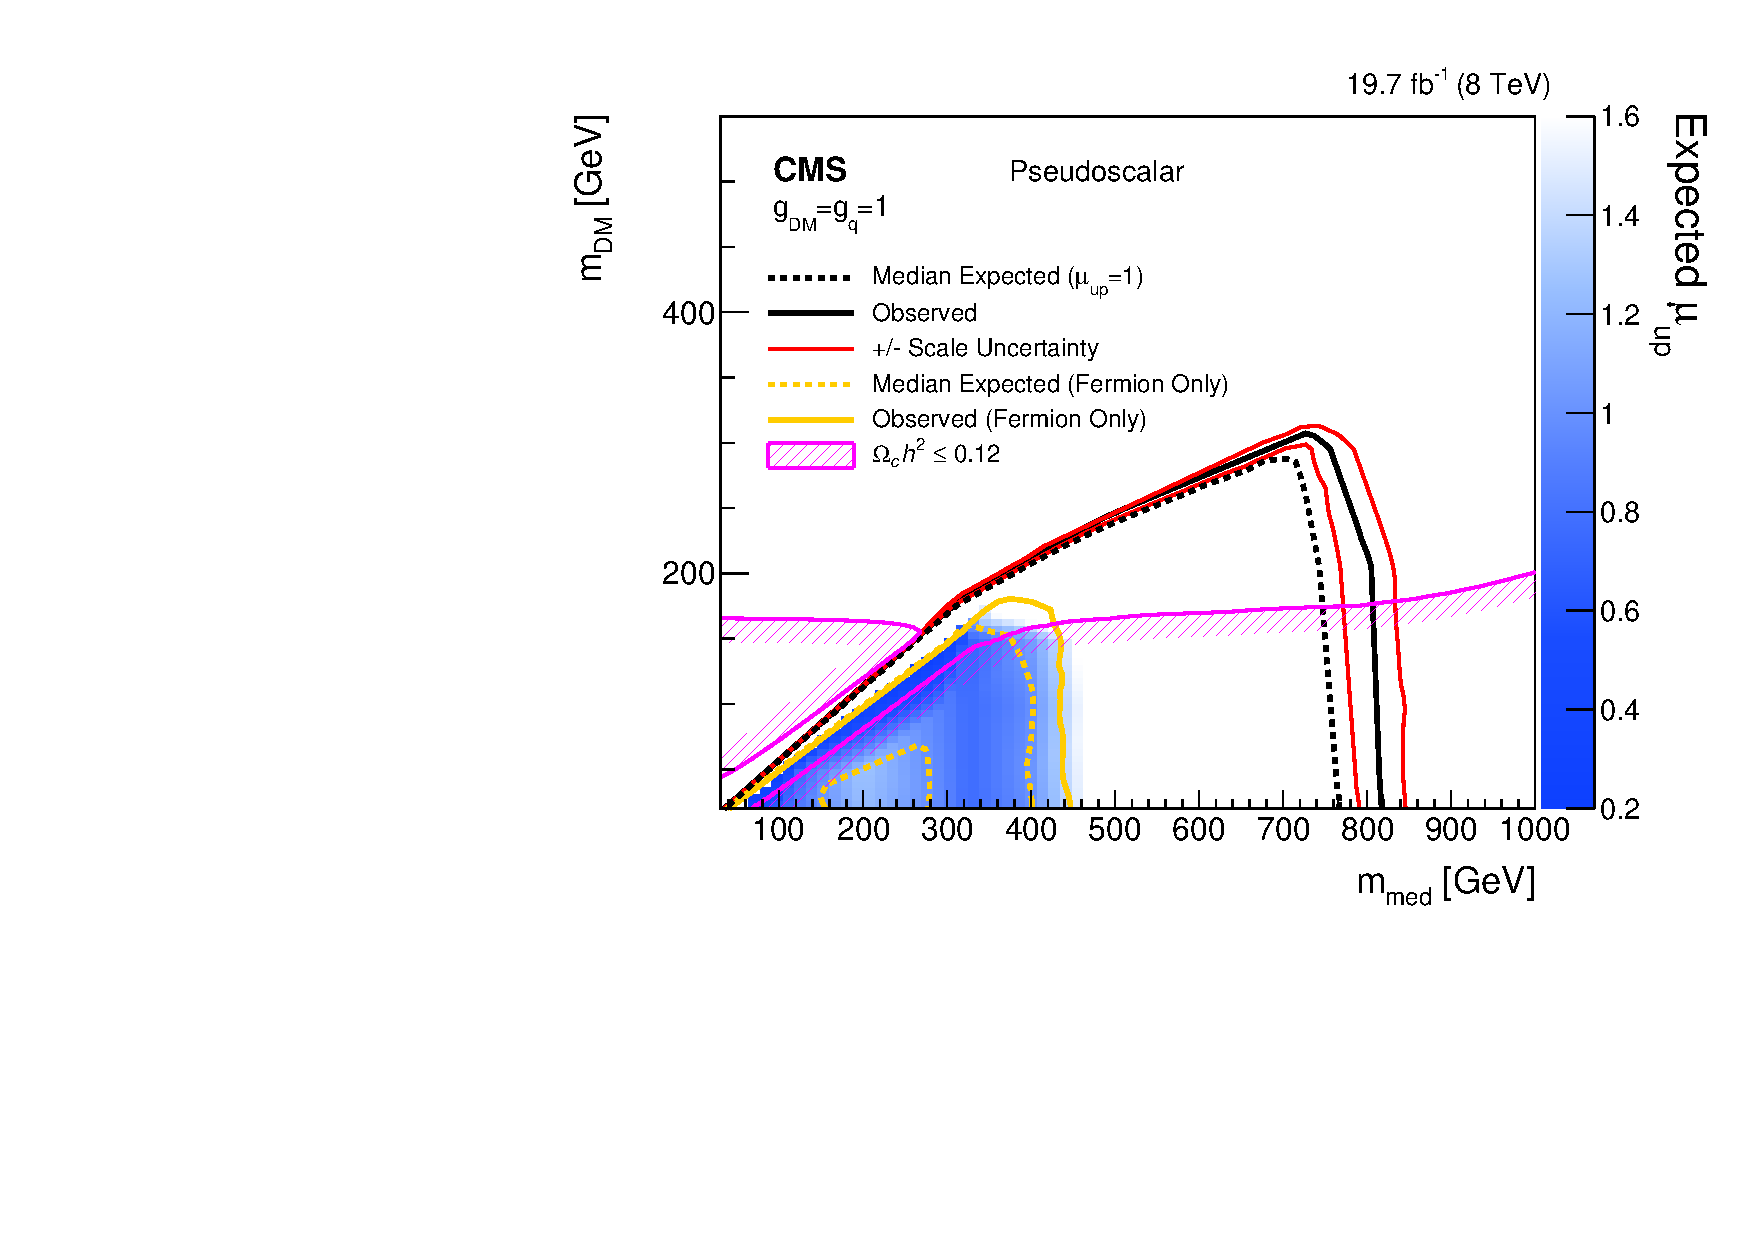
\includegraphics[angle=0,width=0.50\textwidth]{figures/MassLimit_1_806_0_Both.pdf}
\label{fig:mass_806} } \caption{90\% CL exclusion contours in the
$m_{\mathrm{MED}}--m_{\textrm{DM}}$ plane assuming (a) vector, (b) axial vector, 
(c) scalar, and (d) pseudoscalar mediators.  The blue scale shows the expected 
90\% CL exclusion upper limit on the signal strength assuming the mediator only couples to
fermions. For the scalar and pseudoscalar mediators, the exclusion contour
assuming coupling only to fermions (fermionic) is explicitly shown by the orange line. The
white region shows model points which were not tested when assuming coupling
only to fermions and are not expected to be excluded by this analysis under this
assumption.  The excluded region is to the bottom/left of the contours in
all cases, except for that from the relic density as indicated by the shading.
In all of the models, a minimum mediator width is assumed\label{fig:masslims}.}
\end{figure}

Figures~\ref{fig:xslims}(a)--~\ref{fig:xslims}(c) show
the same exclusion contours, this time translated into the plane of
$m_{\textrm{DM}}--\sigma_{\textrm{SI/SD}}$, where $\sigma_{\textrm{SI/SD}}$ are
the spin-independent/spin-dependent (vector and scalar/axial vector) DM-nucleon
scattering cross sections. These representations allow for a more direct
comparison with limits from the DD experiments, which typically set
upper limits on these cross sections~\cite{ Malik:2014ggr,Harris:2015kda}. It
should be noted that the limits set from this analysis are however only valid
under the simplified model considered, and in particular assuming
$g_{\textrm{DM}}=g_{\textrm{SM}}=1$. For the scalar mediator model, it is assumed that
only heavy quarks (top and bottom) contribute. Such a choice limits the
sensitivity for DD experiments, however it allows for direct comparison
between collider and DD experiments without an additional assumption on the
light-quark couplings~\cite{Harris:2015kda}.  For the vector and scalar mediator
models, DD limits are stronger than those obtained in this
analysis except in the scenario where the DM mass is less than around 6
\GeV. For the axial vector mediator model, the limits obtained in this analysis
dominate up to around $m_{\mathrm{DM}}=300$ \GeV. 

For the vector and scalar models, the limits are compared with those from the 
LUX~\cite{Akerib:2012ys} and Super CDMS~\cite{Cheung:2013pfa} experiments. The limits from the LUX experiment currently 
provide the strongest constraints on $\sigma_{\mathrm{SI}}$ for $m_{\rm{DM}} \gtrsim 4$\GeV~\cite{PhysRevLett.116.161301}. 
For axial vector couplings, the limits are compared with DM-proton scattering limits
from the PICO-2L~\cite{Amole:2015lsj}, PICO-60~\cite{Amole:2015pla}, IceCube~\cite{Aartsen:2016exj} and 
Super-Kamiokande~\cite{Choi:2015ara} experiments.  For pseudoscalar interactions, direct
detection bounds are strongly velocity suppressed.  The most appropriate
comparison is therefore to the most sensitive bounds from indirect detection
from the Fermi LAT collaboration~\cite{Ackermann:2011wa,Abdo:2010ex}.  These limits apply to the
scenario in which dark matter is annihilated in the center of a galaxy, producing
a $\gamma$ ray signature.

Under the vector mediator model, the direct detection bounds dominate across
most of the plane, while for the axial vector, there is good complementarity
between the direct detection limits and those from this analysis as shown in Fig.~\ref{fig:xslims}(b). 
Limits in the scalar mediator scenario are more sensitive than those from direct detection for
small DM masses as shown in Fig.~\ref{fig:xslims}(c). 
 
An excess in $\gamma$ ray emmision, consistent with the annihilation of DM, at the galactic 
centre has been reported in several studies using data from Fermi LAT~\cite{Gordon:2013vta,Abazajian:2012pn,Hooper:2010mq}. 
Further studies of this excess suggest that DM 
annihilation could be mediated by a light pseudoscalar~\cite{Calore:2014nla}.  The
production mechanism for these $\gamma$ rays can be interpreted under DM 
annihilation to b quarks allowing for direct comparison with limits from
this analysis~\cite{Buchmueller:2015eea,Buckley:2014fba,Harris:2014hga}.
Figure~\ref{fig:xslims}(d) shows the exclusion contours assuming pseudoscalar
mediation in the plane of DM pair annihilation cross section versus
$m_{\textrm{DM}}$.  Again, it is assumed that only heavy quarks 
contribute in the production of the mediator while for  the
interpretation of the limits in the annihilation cross-section, it is assumed
that the mediator only decays to b quark pairs. 
As with all interpretations, the DM particle is assumed to be a Dirac fermion. 
The results shown from Fermi LAT have been scaled by a factor of 2 compared 
to Ref.~\cite{Ackermann:2011wa} to translate the assumtion of a Majorana DM 
fermion used in that analysis. 
The 68\% CL preferred regions in this plane assuming the annihilation of DM
pairs to light-quarks ($\mathrm{q\bar{q}}$), $\tau^{+}\tau^{-}$ or $\mathrm{b\bar{b}}$, 
using data from Fermi LAT, are shown as solid colour regions. 
For the simplified model used, and assuming that $g_{\mathrm{DM}}=g_{\mathrm{q}}=1$, 
all of these regions are excluded by this analysis. The limits from this analysis are 
stronger than those from Fermi LAT when the DM mass is below 100\GeV.


\begin{figure}[htbp] \centering \subfloat[][]{
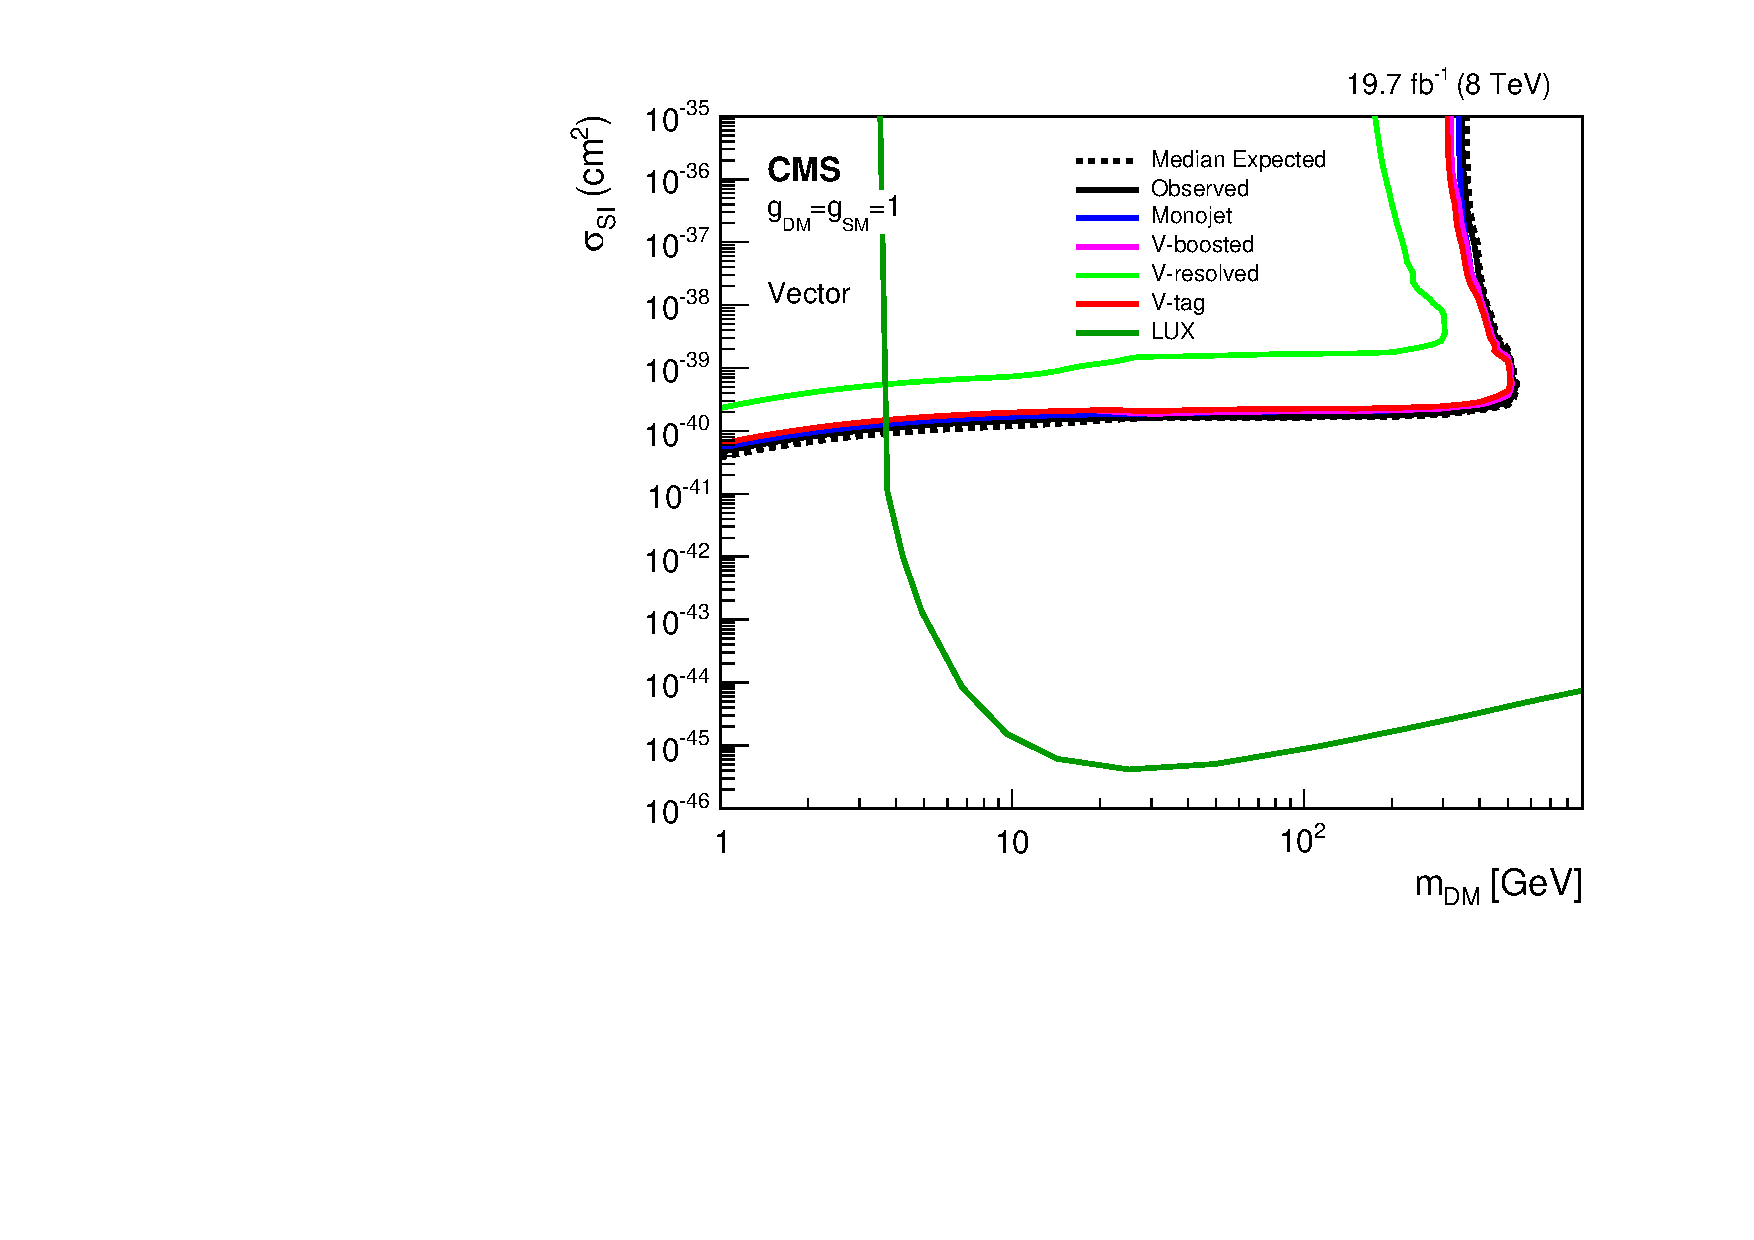
\includegraphics[angle=0,width=0.50\textwidth]{figures/MassLimit_1_800_0_Both_DD.pdf}
\label{fig:xslims_800} } \subfloat[][]{
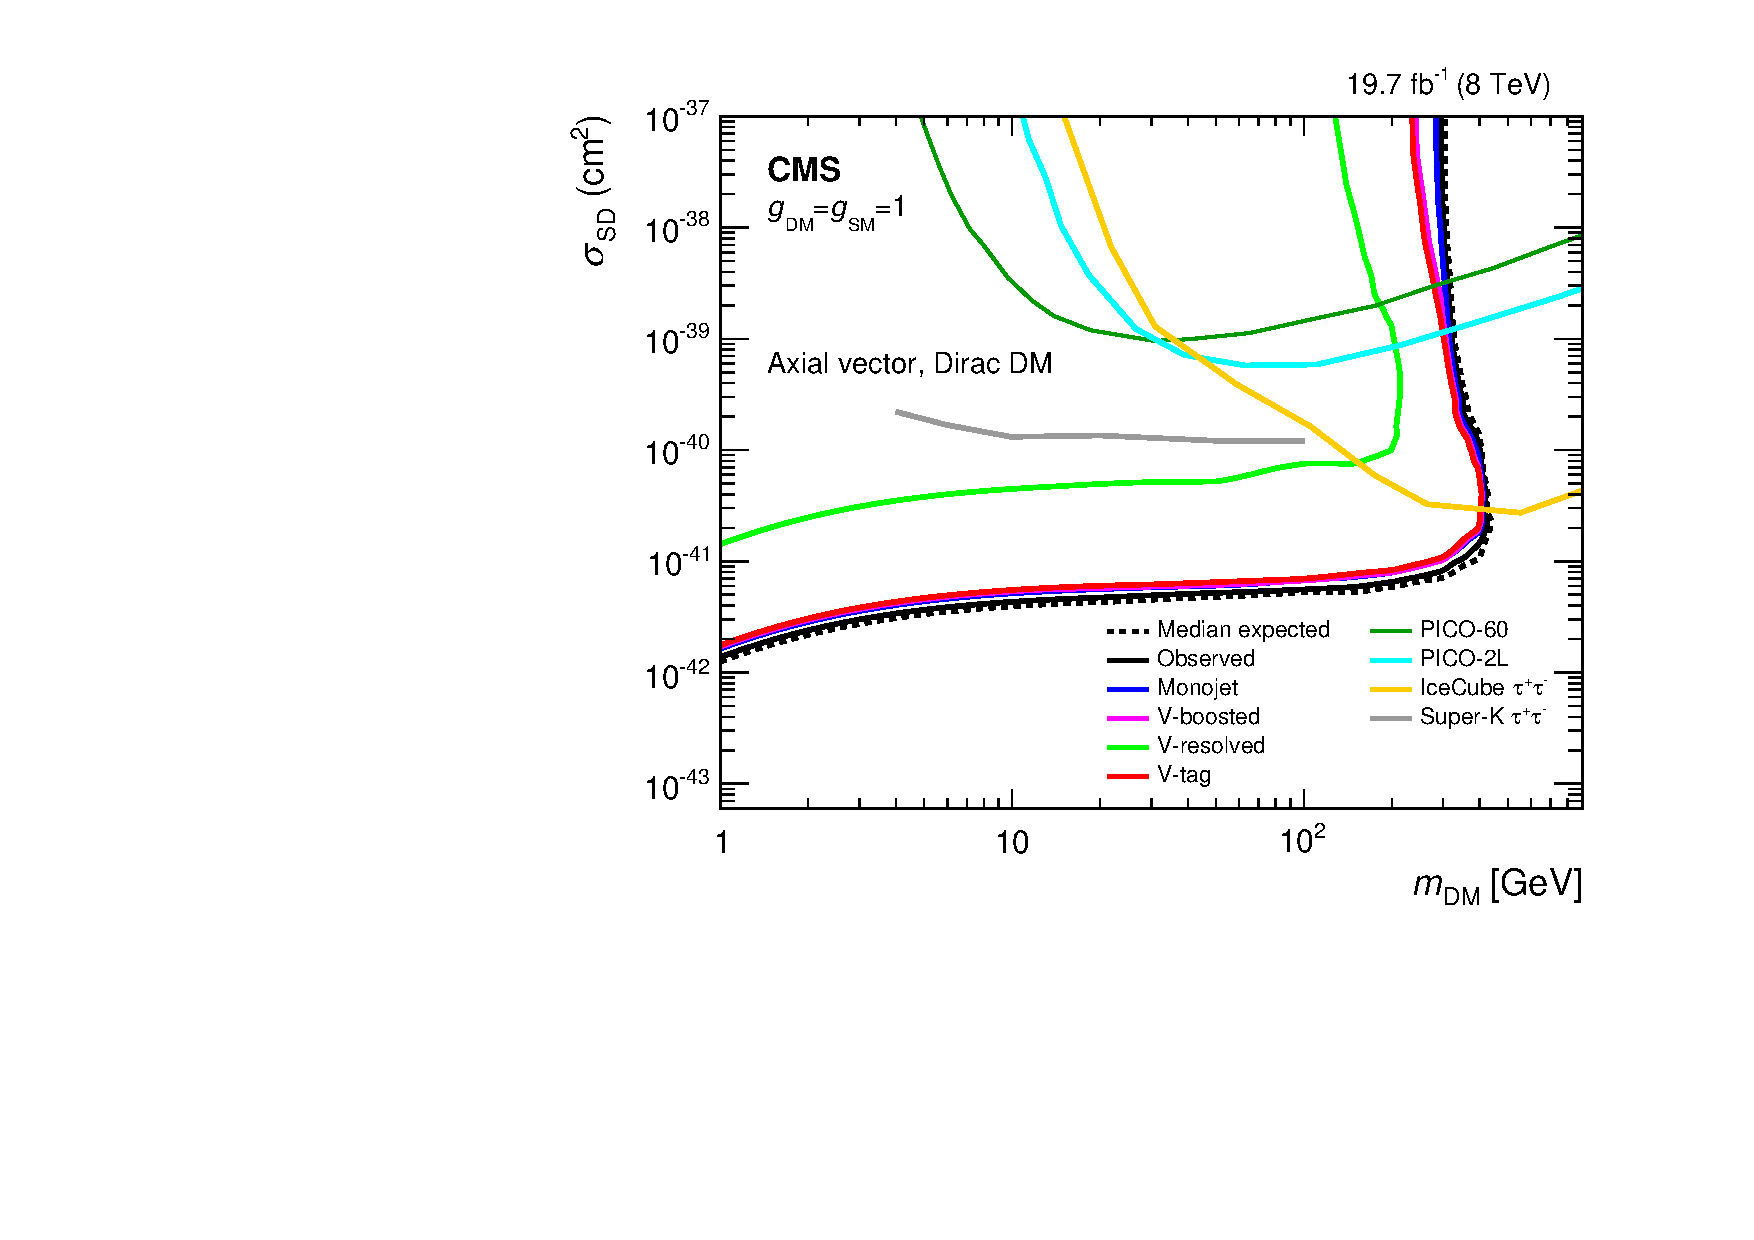
\includegraphics[angle=0,width=0.50\textwidth]{figures/MassLimit_1_801_0_Both_DD.pdf}
\label{fig:xslims_801} }\\ \subfloat[][]{
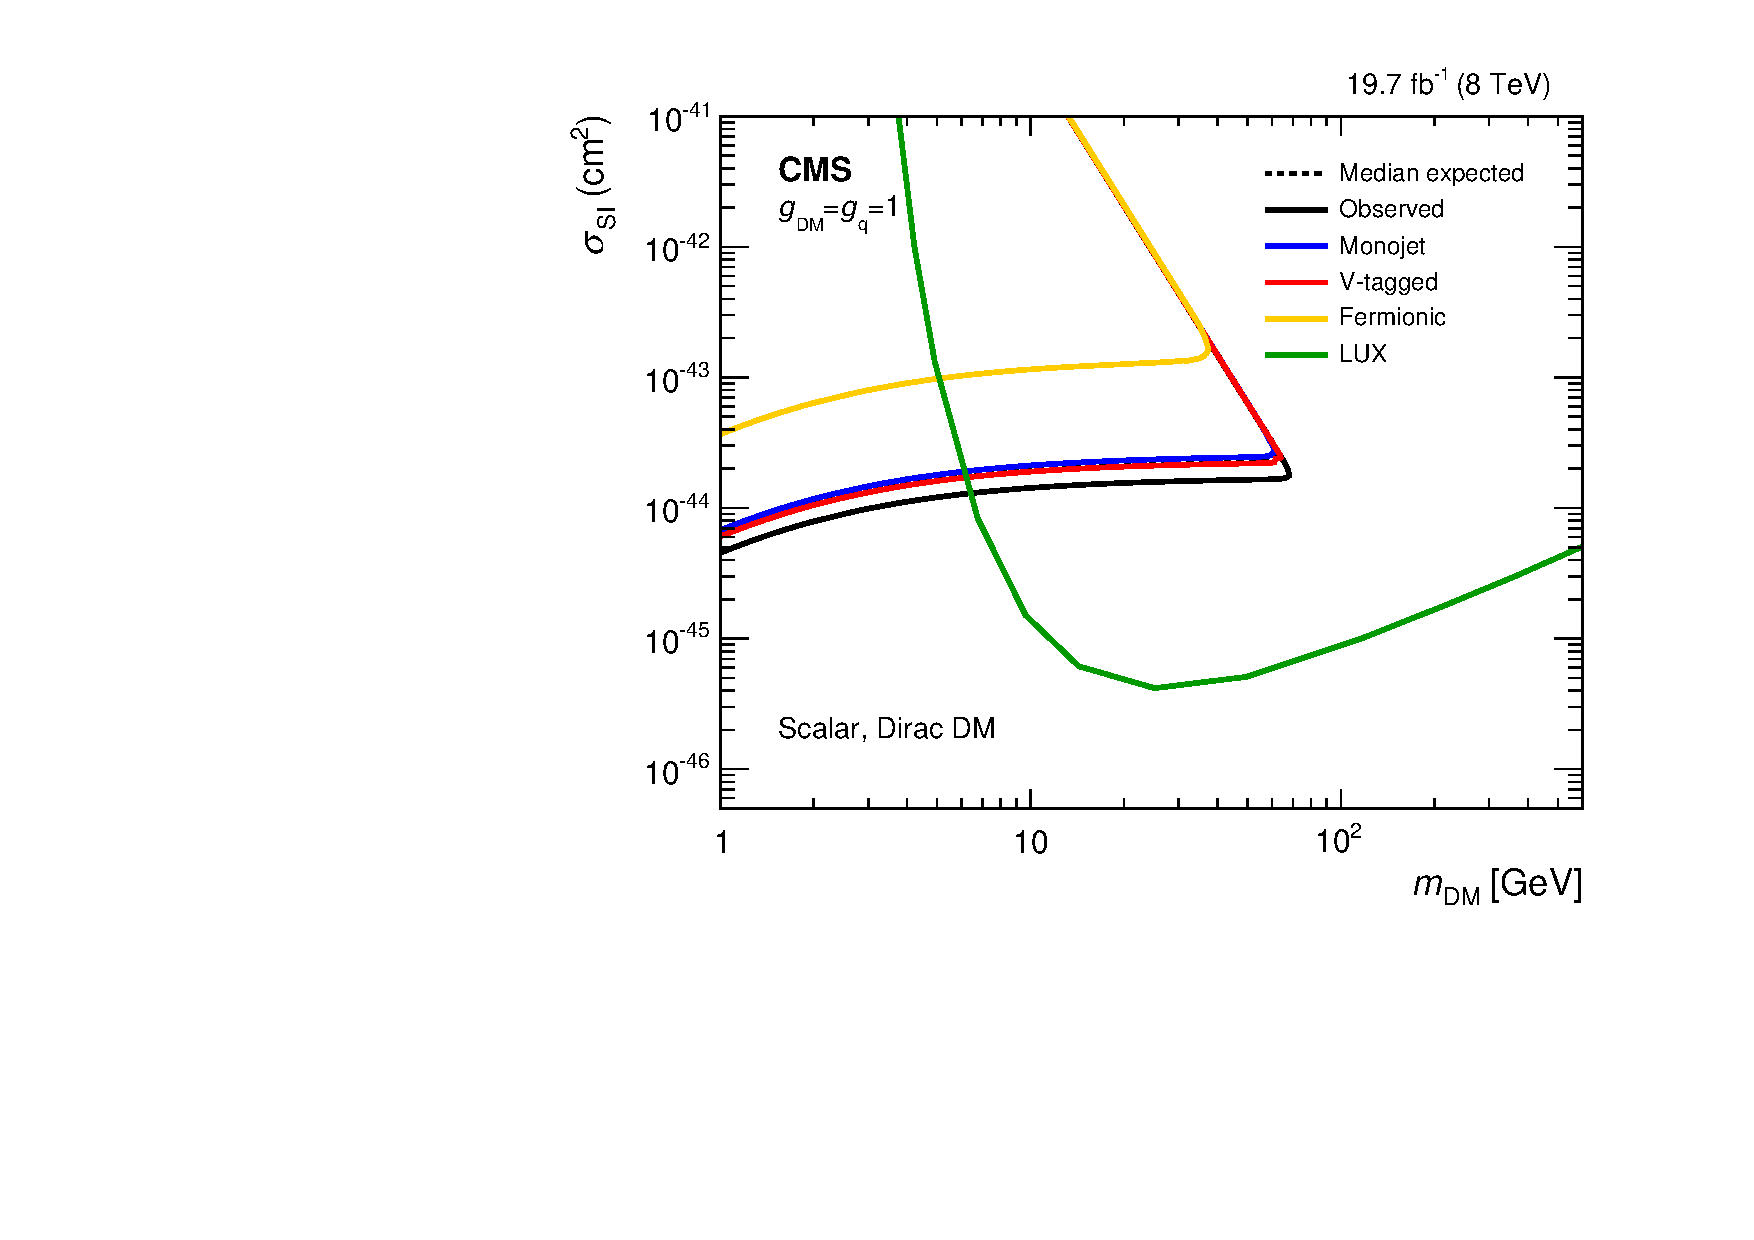
\includegraphics[angle=0,width=0.50\textwidth]{figures/MassLimit_1_805_0_Both_DD.pdf}
\label{fig:xslims_805} } \subfloat[][]{
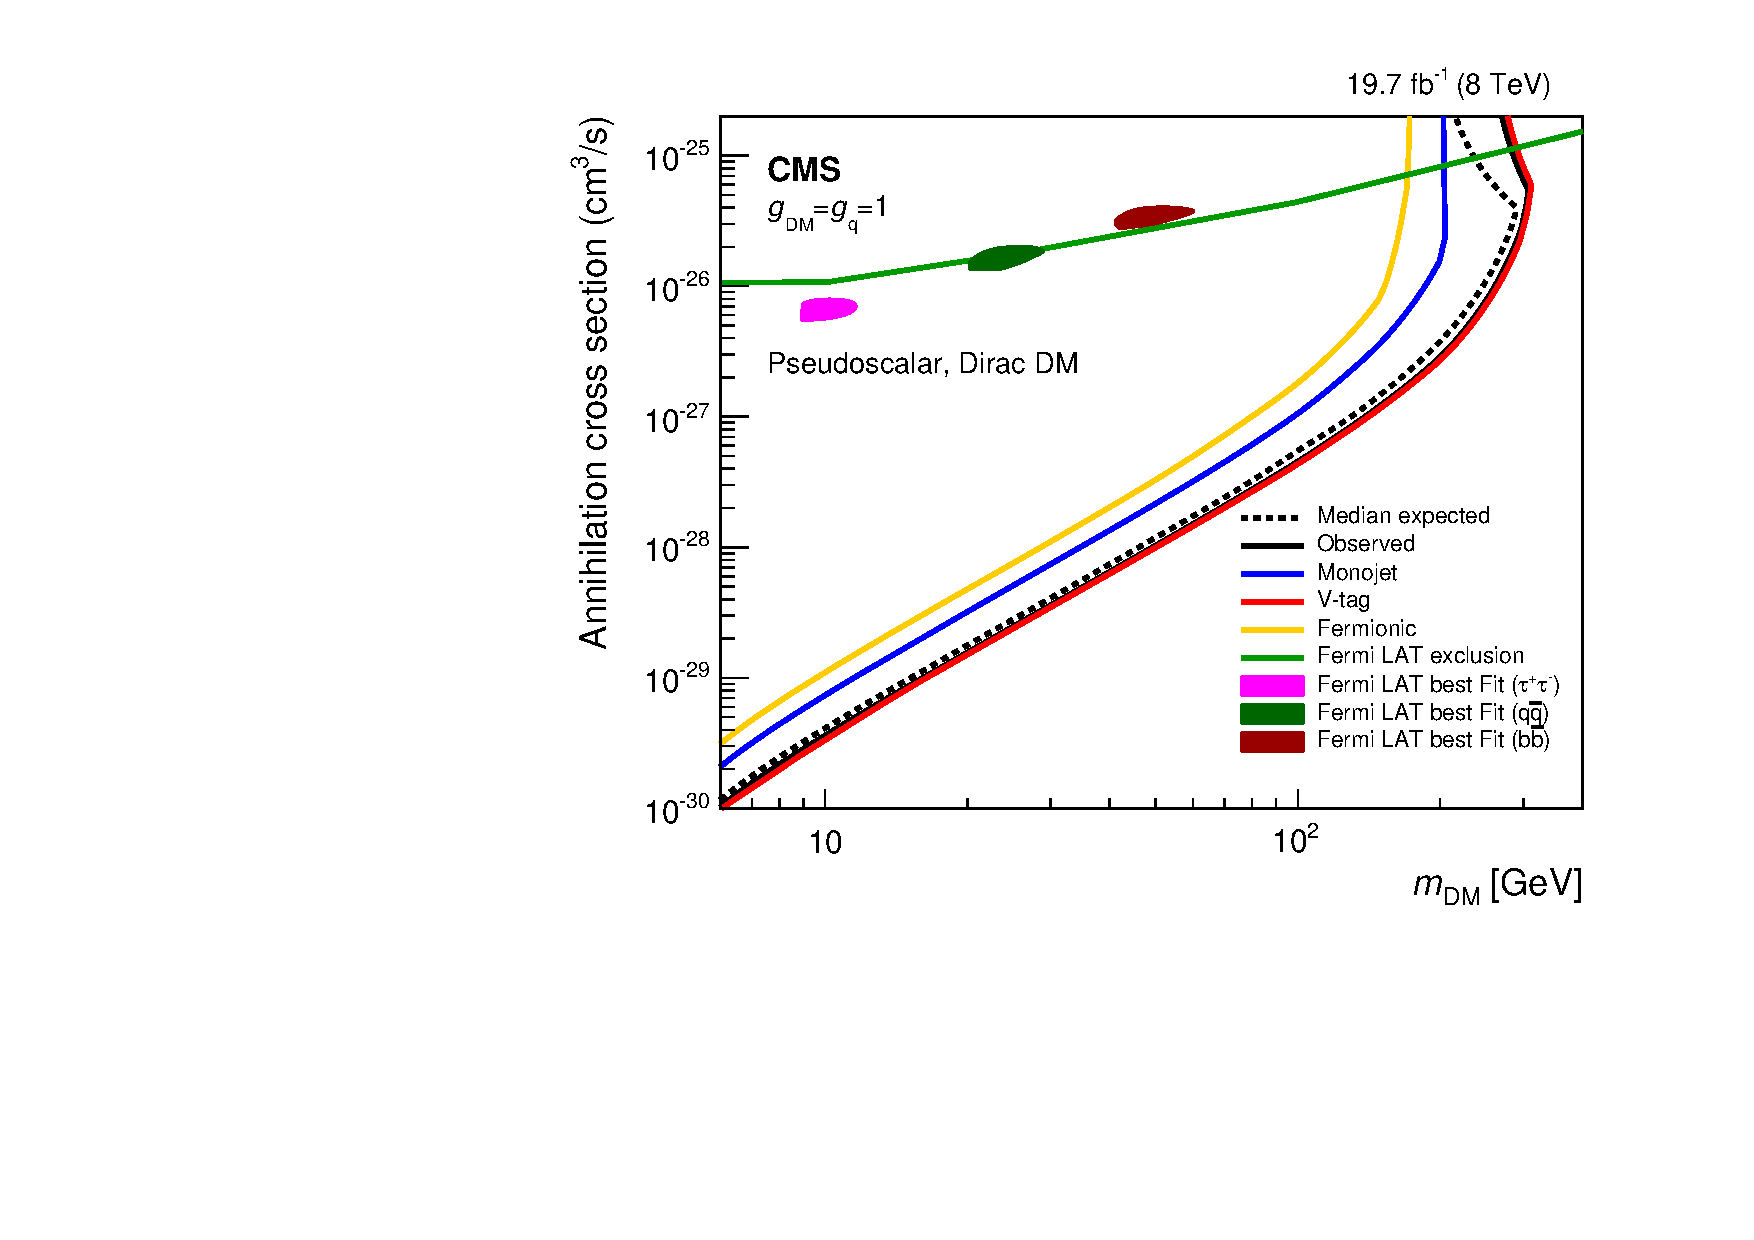
\includegraphics[angle=0,width=0.50\textwidth]{figures/MassLimit_1_806_0_Both_DD.pdf}
\label{fig:xslims_806} } \caption{90\% CL exclusion contours in the
$m_{\textrm{DM}}--\sigma_{\textrm{SI}}$ or $m_{\textrm{DM}}-\sigma_{\textrm{SD}}$ 
plane assuming (a) vector, (b) axial vector, 
(c) scalar mediators. 90\% CL exclusion in DM annihilation cross section as a function of 
$m_{\textrm{DM}}$ for a pseudoscalar mediator. For the scalar and pseudoscalar
case, the orange line shows the exclusion contours assuming the mediator only
couples to fermions (fermionic). The excluded region in all plots is to the top/left of the
contours. In the vector and axial vector scenarios, limits are shown
independently for monojet, V-tagged and V-resolved categories. The partial
combination of the V-tag categories  is
shown for which the V-boosted category provides the dominant contribution.  In all
of the mediator models, a minimum mediator width is assumed. For the pseudoscalar, 68\%
CL preferred regions, using data from Fermi LAT, for DM annihilation to
light-quarks ($\mathrm{q\bar{q}}$), ($\tau^{+}\tau^{-}$) and $\mathrm{b\bar{b}}$ are shown
by the solid green, pink and brown coloured regions, respectively.\label{fig:xslims} } 
\end{figure}

\clearpage
\section{Summary} 
A search has been presented for an excess of events with a
energetic jet in association with large missing transverse energy in a
data sample of proton-proton interactions at centre-of-mass energy of 8 TeV. The
data correspond to an integrated luminosity of 19.7\fbinv collected with the CMS
detector at the LHC.  This search is the first at CMS to utilise jet sub-structure
techniques in order to identify hadronically decaying vector bosons in both
Lorentz-boosted and resolved scenarios. Sensitivity to a potential mono-V signature is
achieved by the addition of two event categories which select hadronically decaying vector
boson using novel jet substructure techniques. 
The sensitivity of the search has been increased compared to the previous CMS result by using
the full shape of the $\ETm$ distribution to discriminate signal from standard
model backgrounds.  No significant deviation from the expectation from
standard model backgrounds is observed in the \ETm distributions.  The results of the search
are interpreted under a set of simplified models which describe the production
of dark matter via vector, axial vector, scalar or pseudoscalar mediation and constraints
on the parameter space of these simplified models are produced. The search is
the first at CMS to be interpreted under these simplified models for
DM production. 

\clearpage
%\appendix
%\section{Alternative Analyses}

Two alternative analyses were implemented in order to provide a cross-check of the 
modelling for the V+jets backgrounds described in section~\ref{sec:zjetsmodel}. 
For both analyses the selection and categorisation of the events 
are identical to the baseline analysis. In addition, the definitions of the control regions 
are also that used for the baseline analysis. All of the systematics described in the main text 
are also included in both analyses, though their effect is re-evaluated for each alternative analysis. 

\subsubsection{Parametric analysis}

In order to further constrain the tails of the distributions of \ETm in the V+jets backgrounds, the low and high ends 
of the spectrum can be correlated through the use of a parametric function. In this analysis, the high statistics 
of the lower \ETm events is exploited and the shape extrapolated to the high \ETm events. 
The \ETm distributions of the \Zvvjets~events and \Wlvjets~events in the signal region are parameterized as the sum of two exponential functions in the 
monojet category whereas for the boosted and resolved categories, due to the lower statistics 
in these categories, a single power law is used. An unbinned fit of these functions is first performed to the simulated Z+jets or W+jets events 
in the signal region.
Taking one event category, for each bin in fake \ETm, the number of expected events in each of the three 
control regions can be expressed as, 
\begin{equation}
N^{Z_{\mu\mu}/\gamma }_{i} (\boldsymbol{\alpha})=  \dfrac{1}{R^{Z/\gamma}_{i}} \int_{\mathrm{Bin_i}} f(\boldsymbol{\alpha},\ETm),
\end{equation} 
for the dimuon and photon plus jet control regions and,
\begin{equation}
N^{W}_{i}(\boldsymbol{\beta}) =  \dfrac{1}{R^{W}_{i}} \int_{\mathrm{Bin_i}} g(\boldsymbol{\beta},\ETm),
\end{equation} 
for the single muon control region, where $\boldsymbol{\alpha}$ and $\boldsymbol{\beta}$ are the free parameters 
of the double exponential or power law functions used to parameterize the\ETm spectrum of the 
 $\Zvvjets$ ($f$) and $\Wlvjets$ ($g$) backgrounds.
 The likelihood for each category then becomes,

\begin{align*}
\mathcal{L}_{\textrm{c}}(\boldsymbol{\alpha}^{\textrm{c}}\boldsymbol{\beta}^{\textrm{c}},\boldsymbol{\theta},\boldsymbol{\phi}) &=        
                \prod_{i} \mathrm{Possion}(d^{\textrm{c},\gamma}_{i} |B^{\textrm{c},\gamma}_{i}(\boldsymbol{\phi}) +\int_{\mathrm{bin}_{i}} \frac{1}{R^{\textrm{c},\gamma}_{i}(\boldsymbol{\theta})} f^{\textrm{c}}(\boldsymbol{\alpha}^{c},E_{T}^{miss})   ) \\
       &~\times \prod_{i} \mathrm{Possion}(d^{\textrm{c},Z}_{i}      |B^{\textrm{c},Z}_{i}(\boldsymbol{\phi})      +\int_{\mathrm{bin}_{i}} \frac{1}{R^{\textrm{c},Z}_{i}(\boldsymbol{\theta})} f^{\textrm{c}}(\boldsymbol{\alpha}^{c},E_{T}^{miss})        ) \\
       &~\times \prod_{i} \mathrm{Possion}(d^{\textrm{c},W}_{i}     |B^{\textrm{c},W}_{i}(\boldsymbol{\phi})      +\int_{\mathrm{bin}_{i}} \frac{1}{R^{\textrm{c},W}_{i}(\boldsymbol{\theta})} g^{\textrm{c}}(\boldsymbol{\beta}^{c},E_{T}^{miss})        ) \\
\end{align*}
where the constrained nuisance parameters $\boldsymbol{\theta}$ and $\boldsymbol{\phi}$ are the same as in the 
baseline analysis and the superscript ``c'' indicates components uncorrelated between categories.
The full likelihood is again a product of $\mathcal{L}_{\textrm{c}}$ over the three event categories.

As with the baseline analysis, the likelihood is maximised (fit) with respect to the parameters, this time being 
those of the parametric function, $\boldsymbol{\alpha}^{c}$ and $\boldsymbol{\beta}^{c}$  
 and the nuisance parameters. 
The ratio of the functions $f^{\textrm{c}}(\ETm)$ and $g^{\textrm{c}}(\ETm)$ at the values of the parameters which maximise the 
likelihood to that before the fit provides a correction as a function of \ETm which can be used to re-weight the Z+jets and W+jets simulation in the 
signal region. The results of the fit are shown in 
Figure~\ref{fig:combined_fit_result_mbin}.

\begin{figure*}[hbtp]\begin{center}
 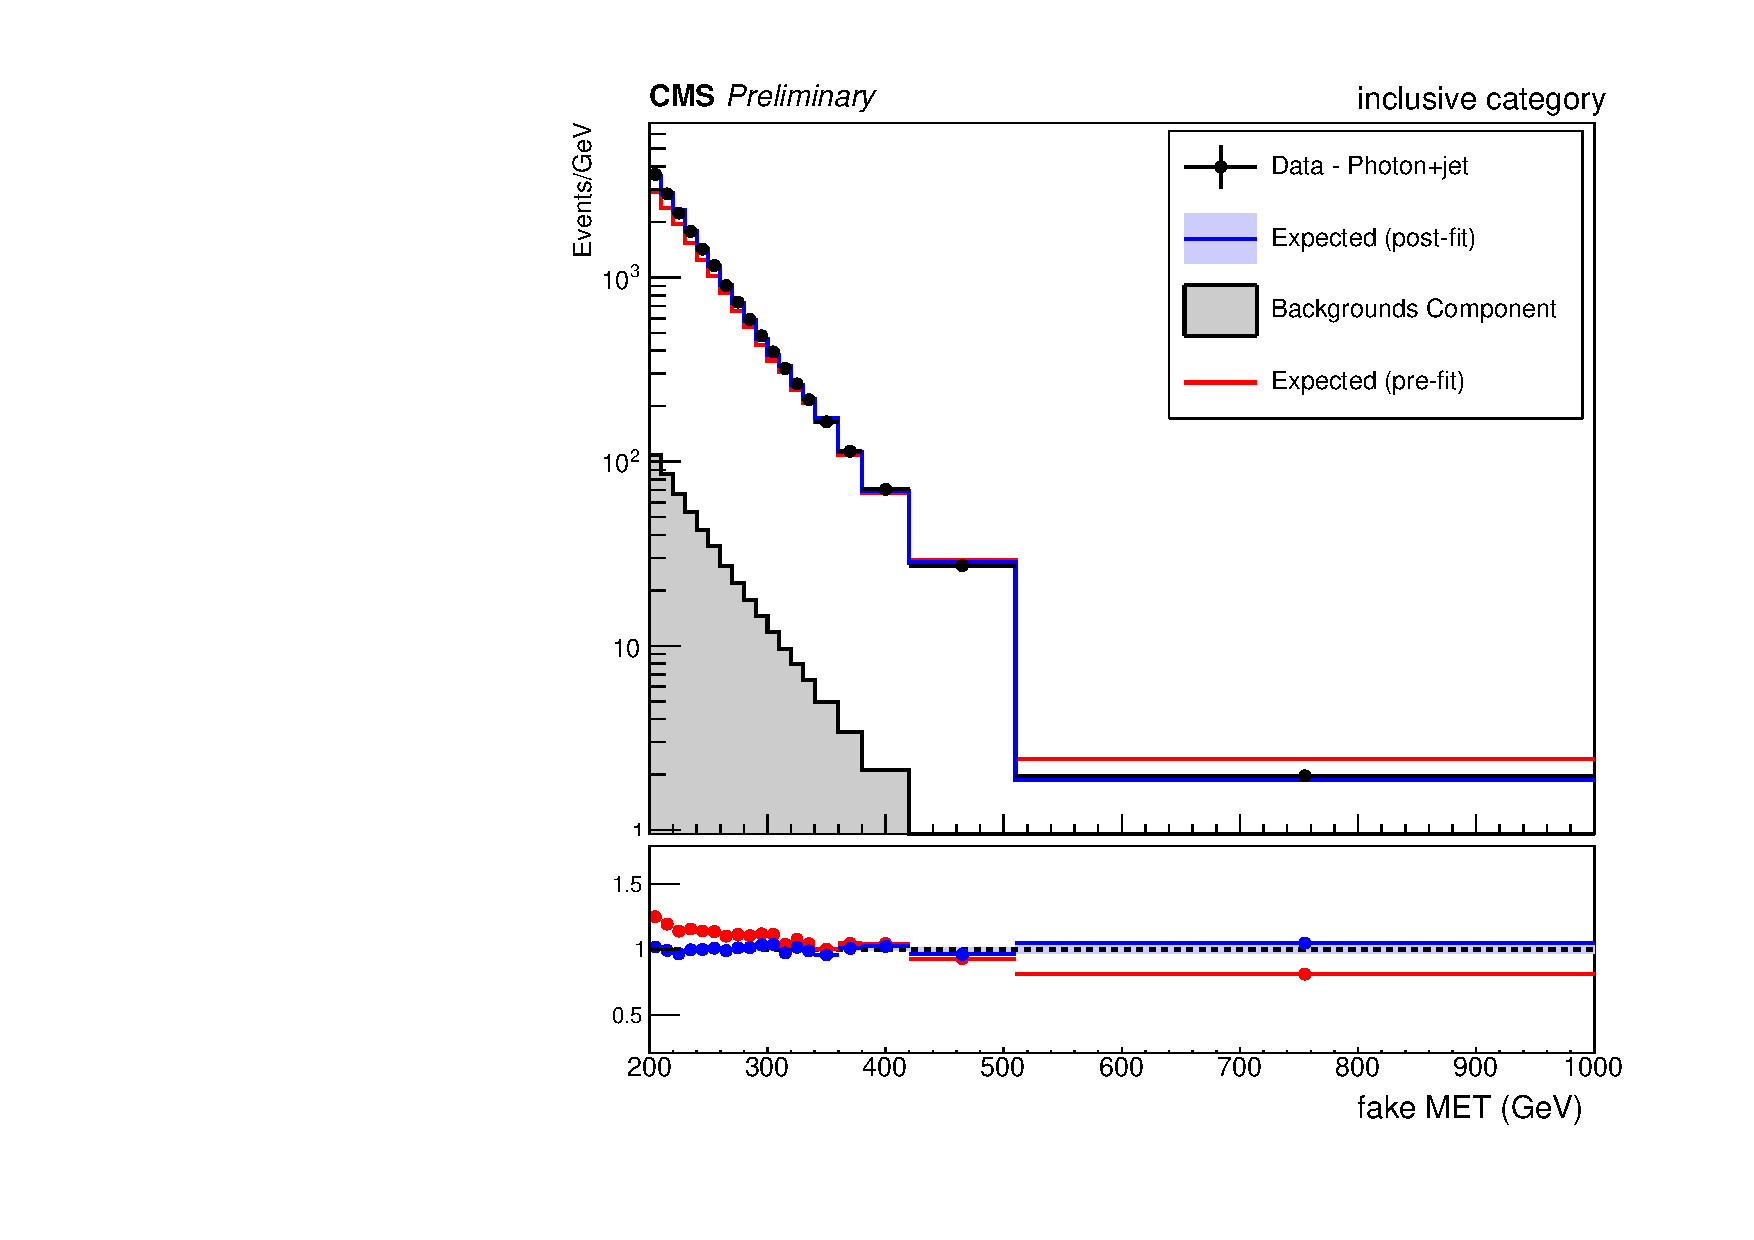
\includegraphics[width=0.32\textwidth]{fig/post_fit_photon_inclusive.pdf}
 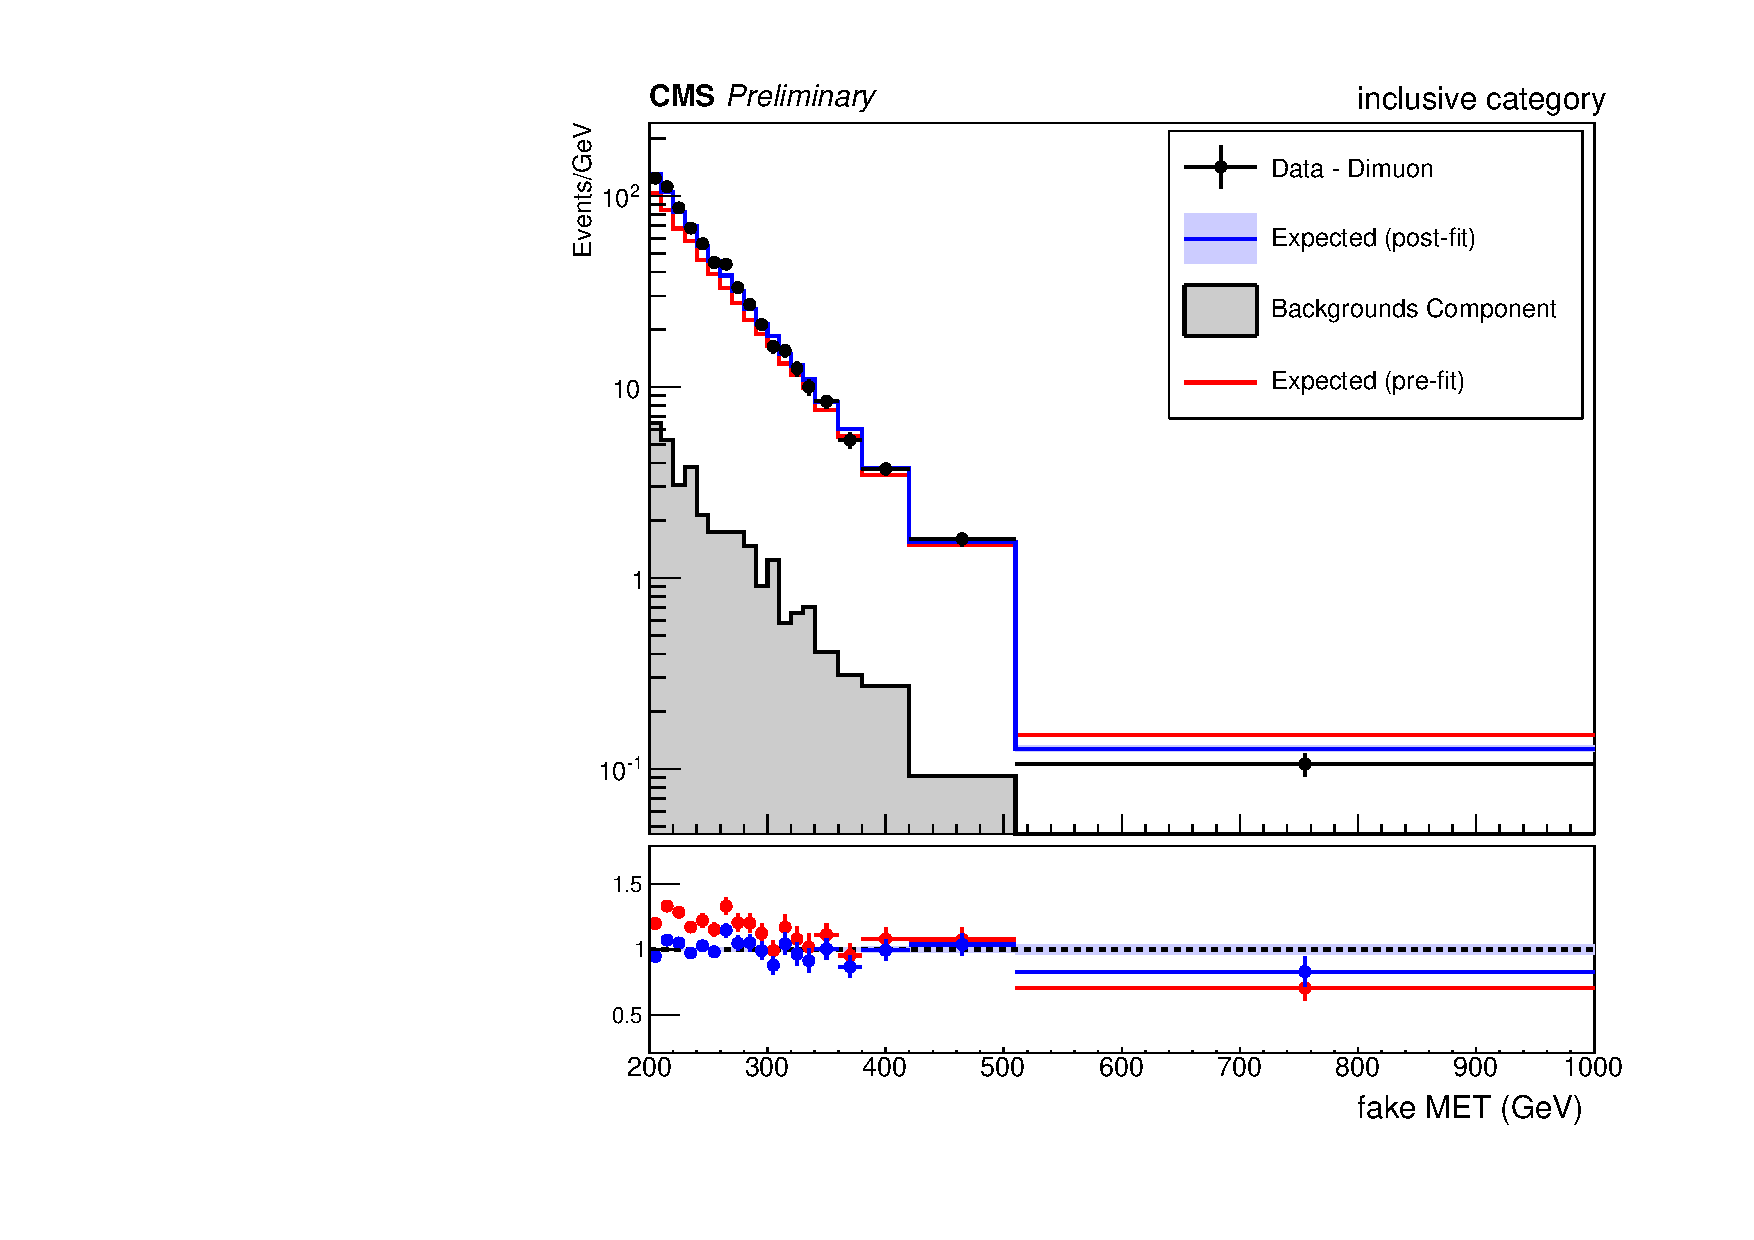
\includegraphics[width=0.32\textwidth]{fig/post_fit_zmm_inclusive.pdf}
 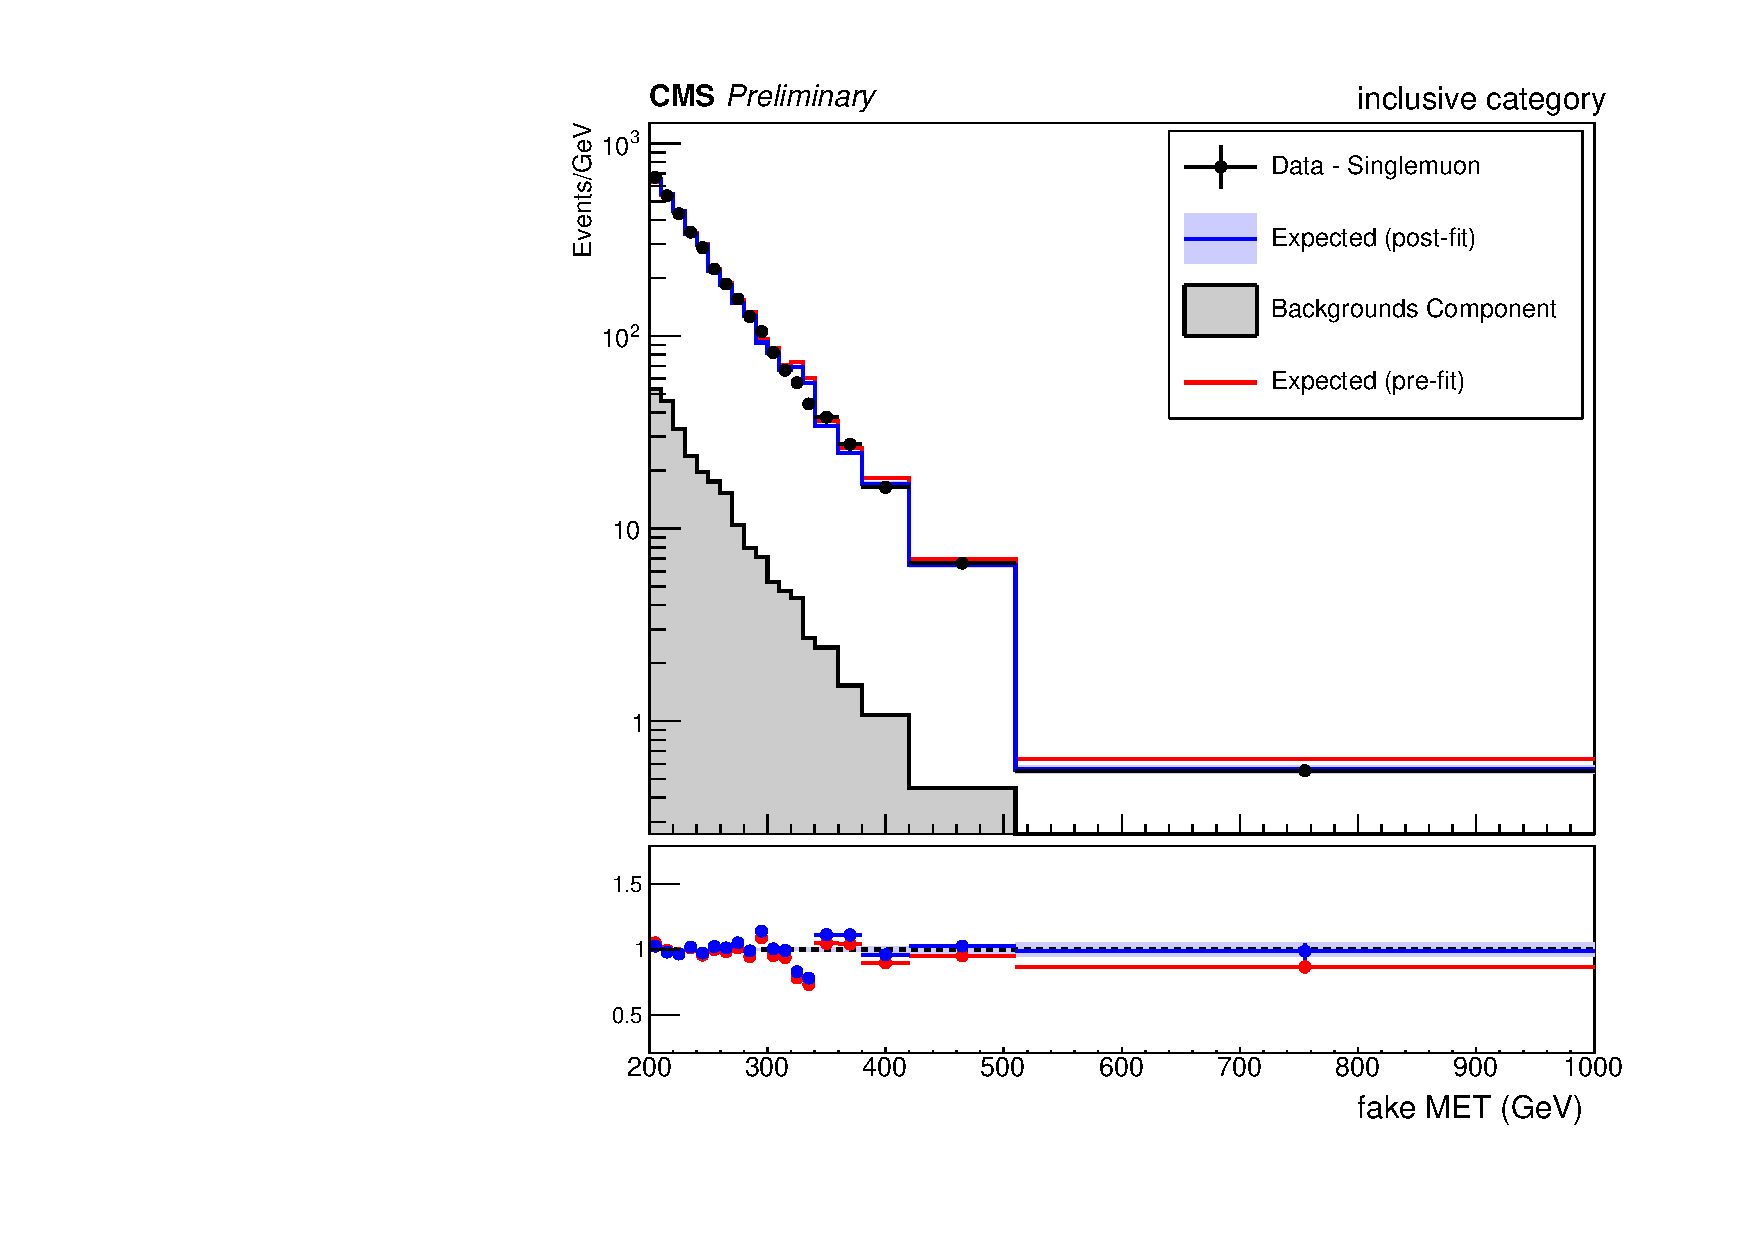
\includegraphics[width=0.32\textwidth]{fig/post_fit_wmn_inclusive.pdf}\\
 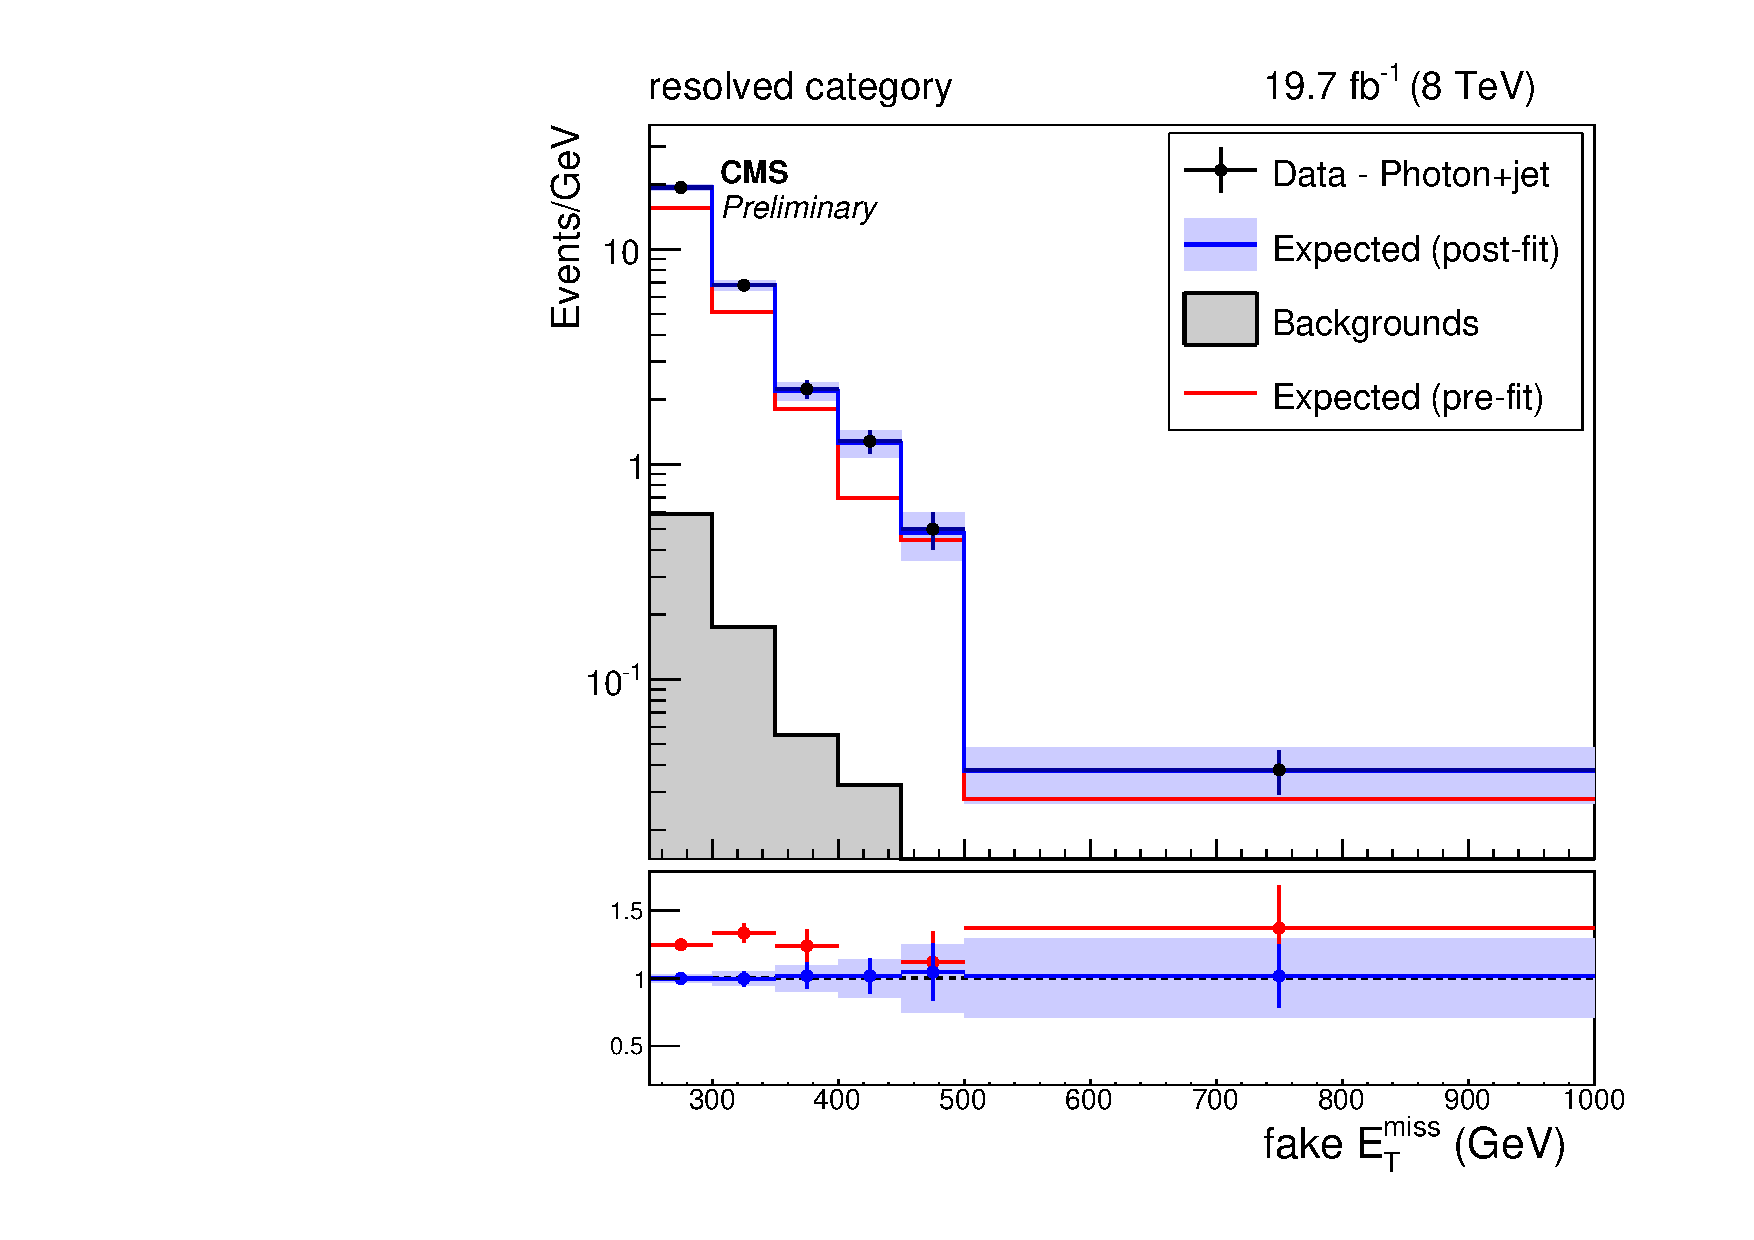
\includegraphics[width=0.32\textwidth]{fig/post_fit_photon_resolved.pdf}
 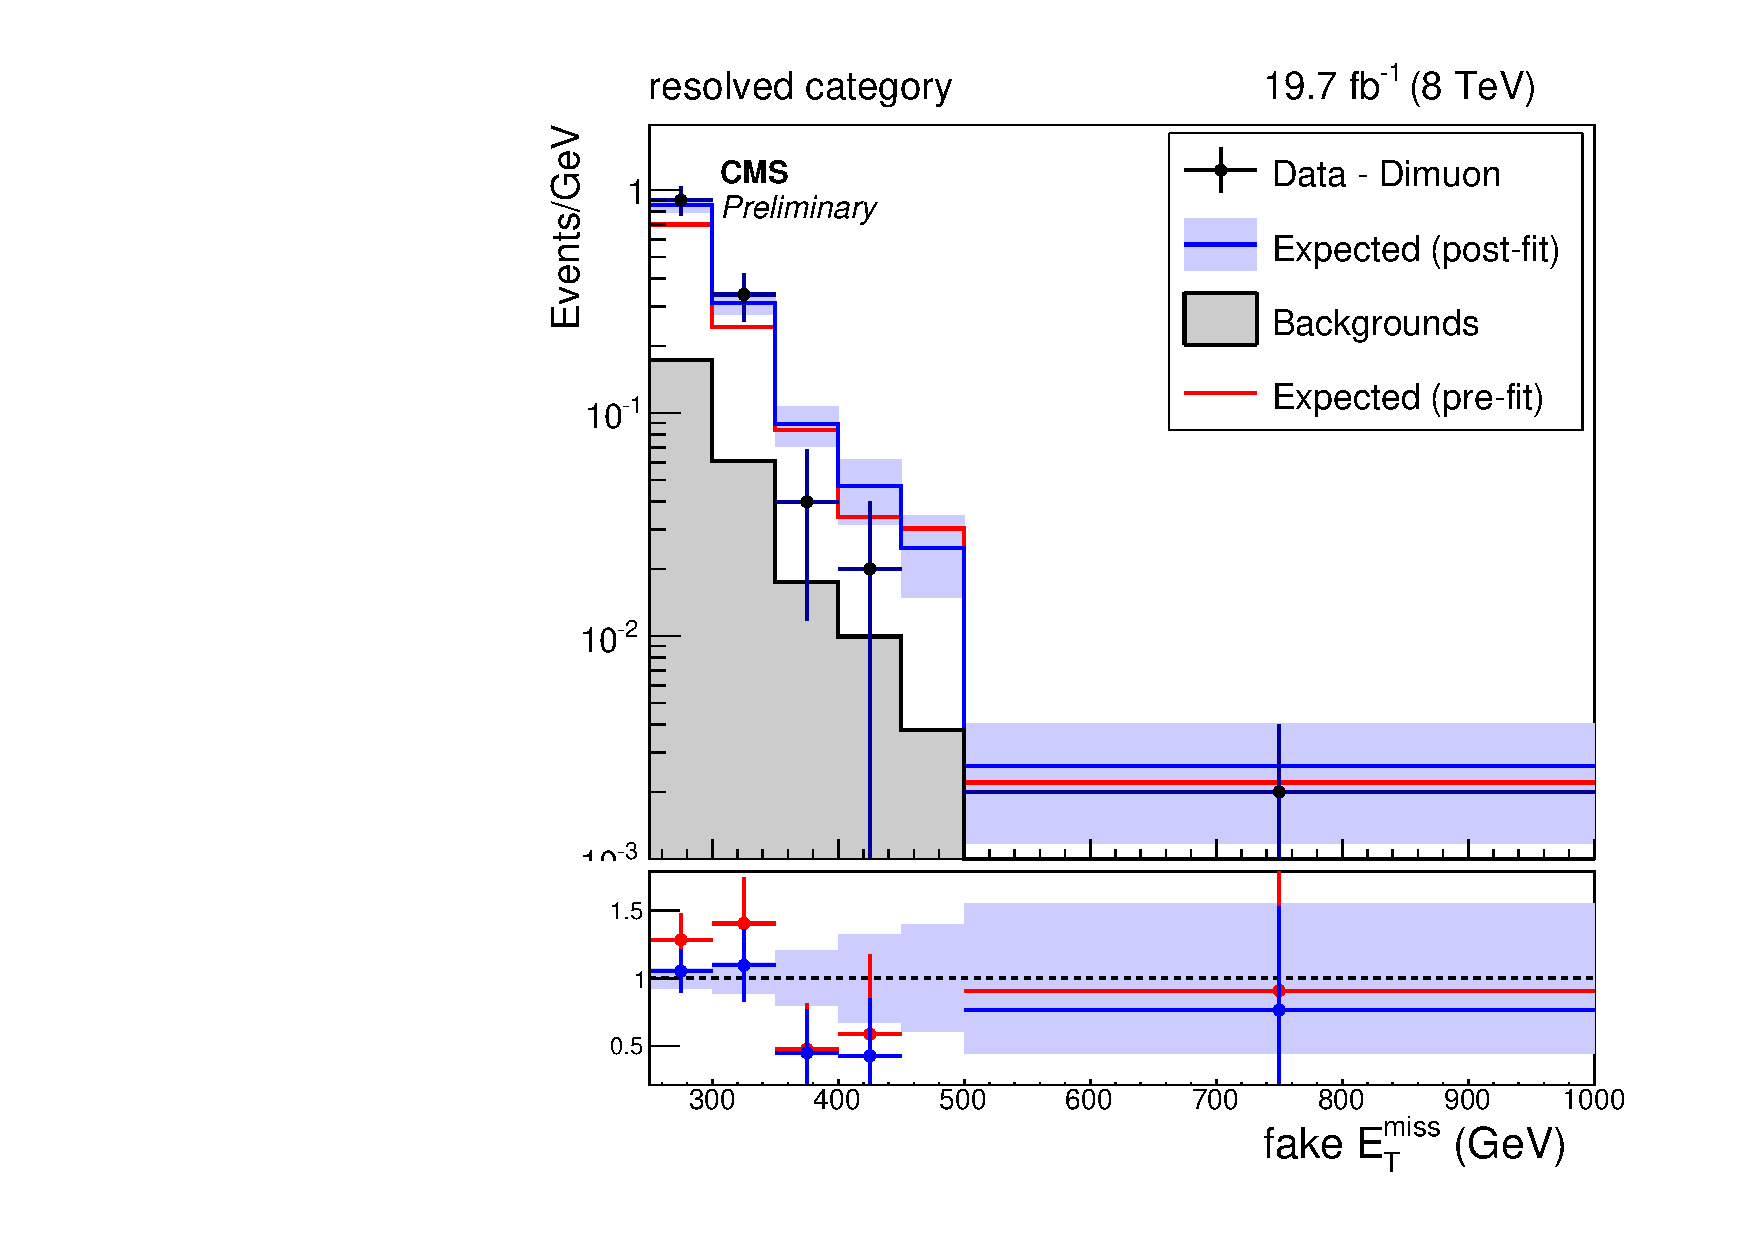
\includegraphics[width=0.32\textwidth]{fig/post_fit_zmm_resolved.pdf}
 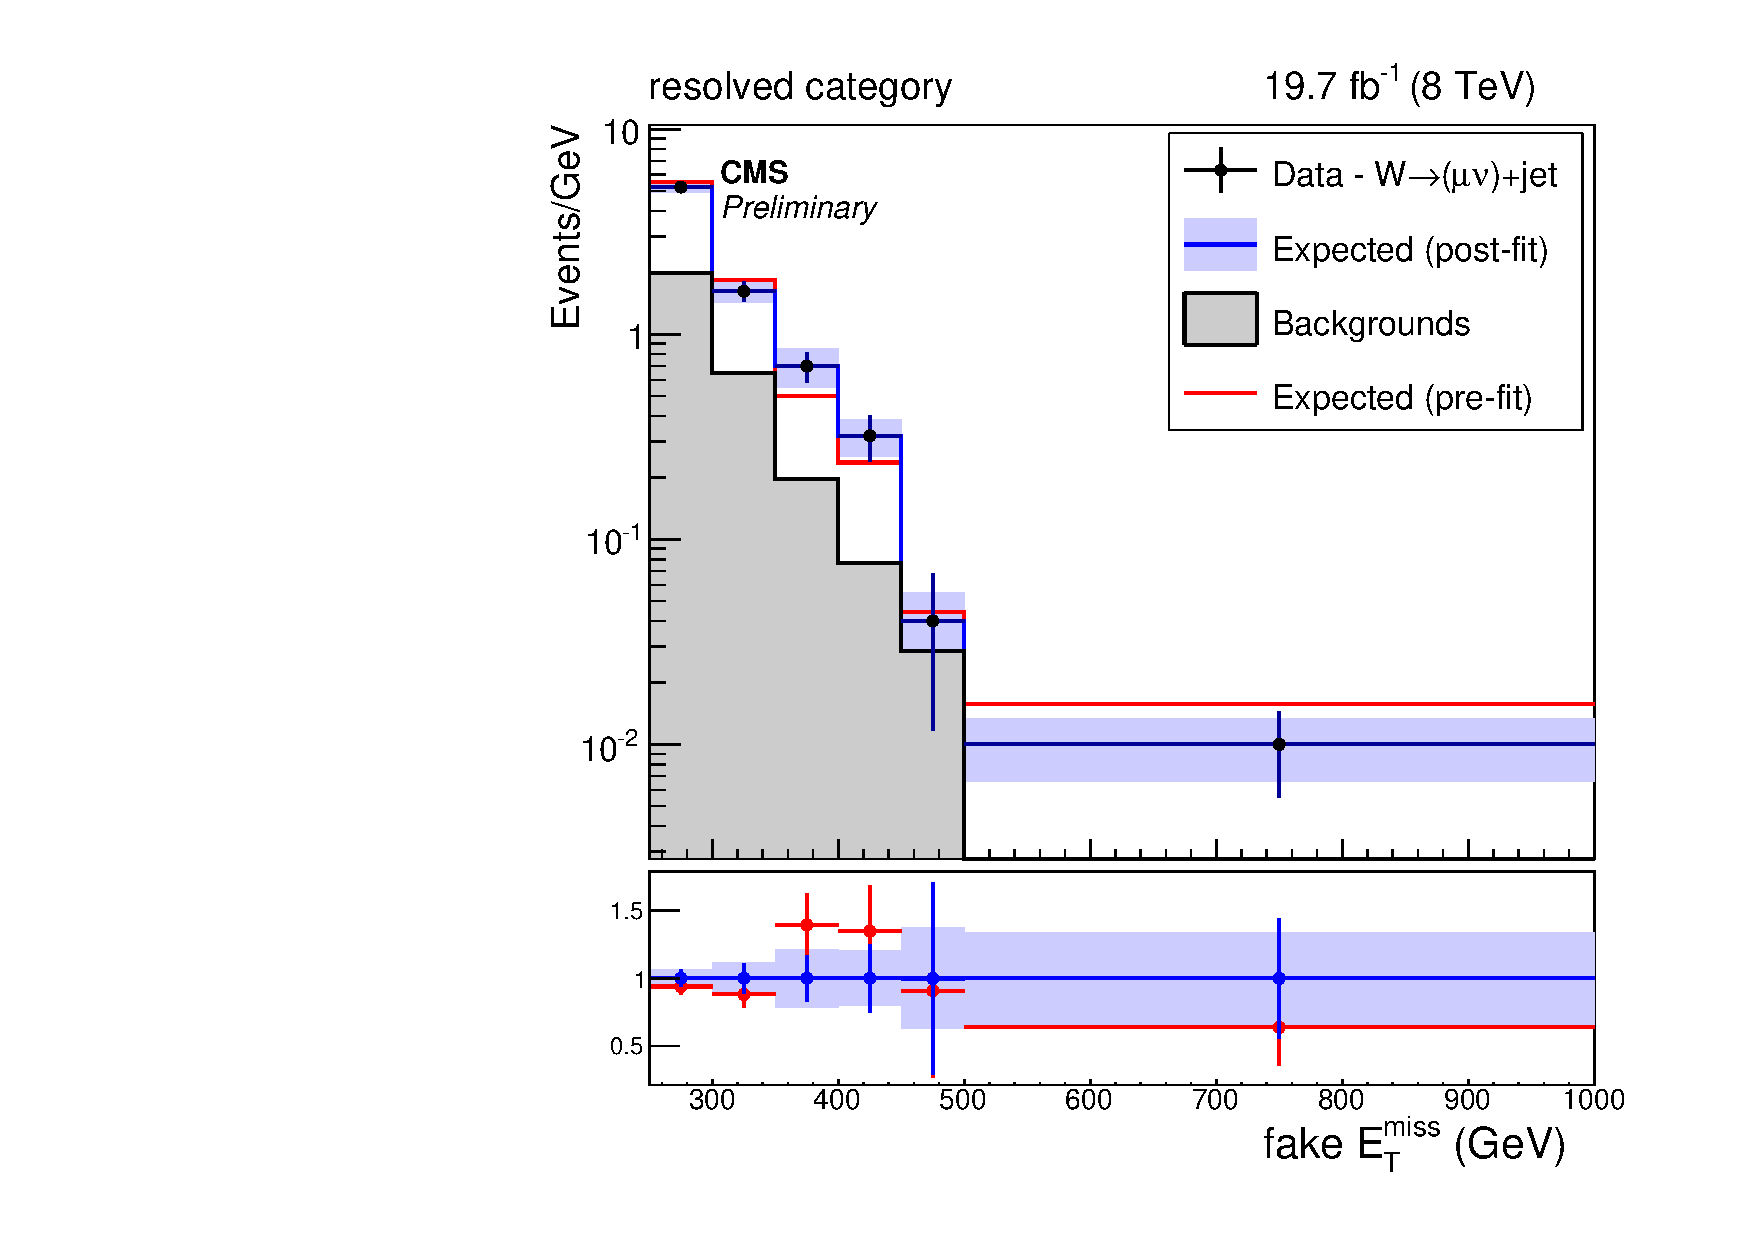
\includegraphics[width=0.32\textwidth]{fig/post_fit_wmn_resolved.pdf}\\
 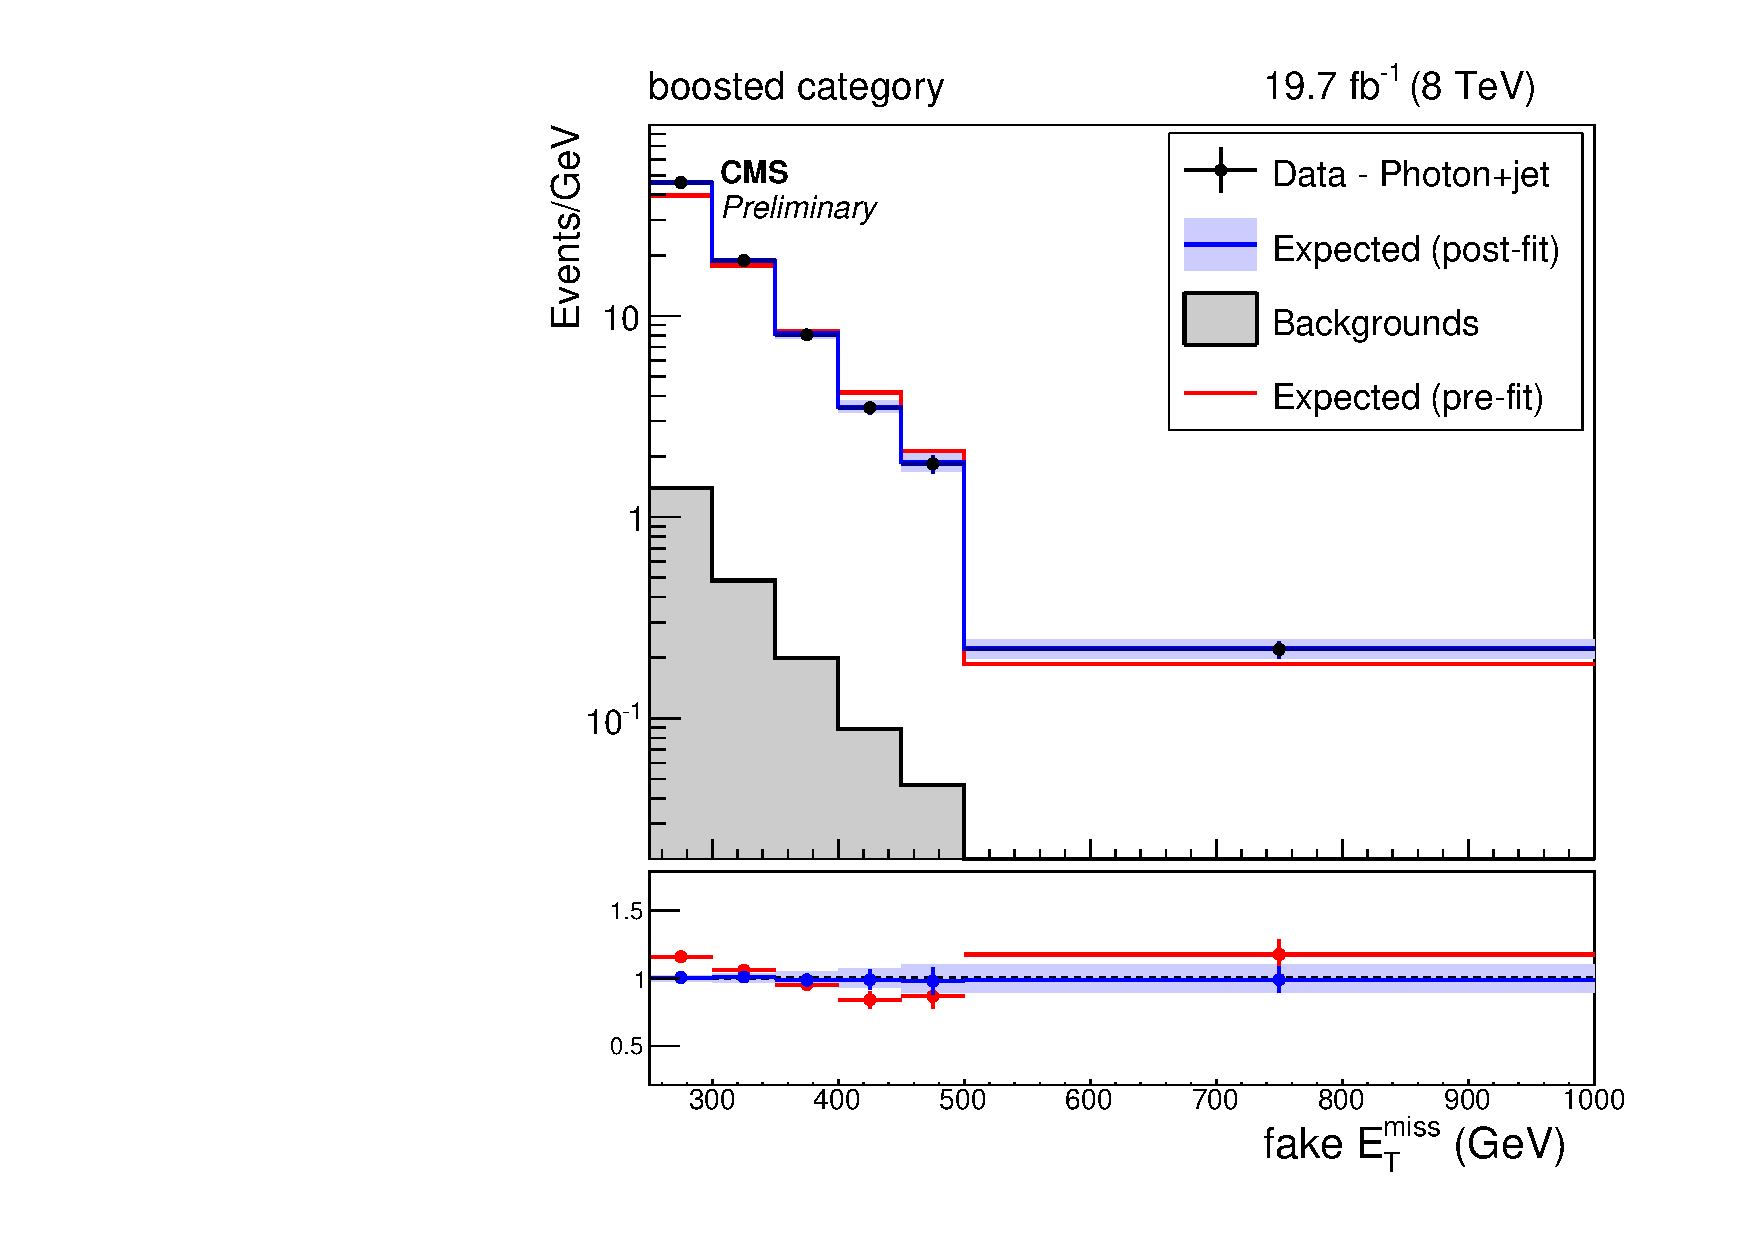
\includegraphics[width=0.32\textwidth]{fig/post_fit_photon_boosted.pdf}
 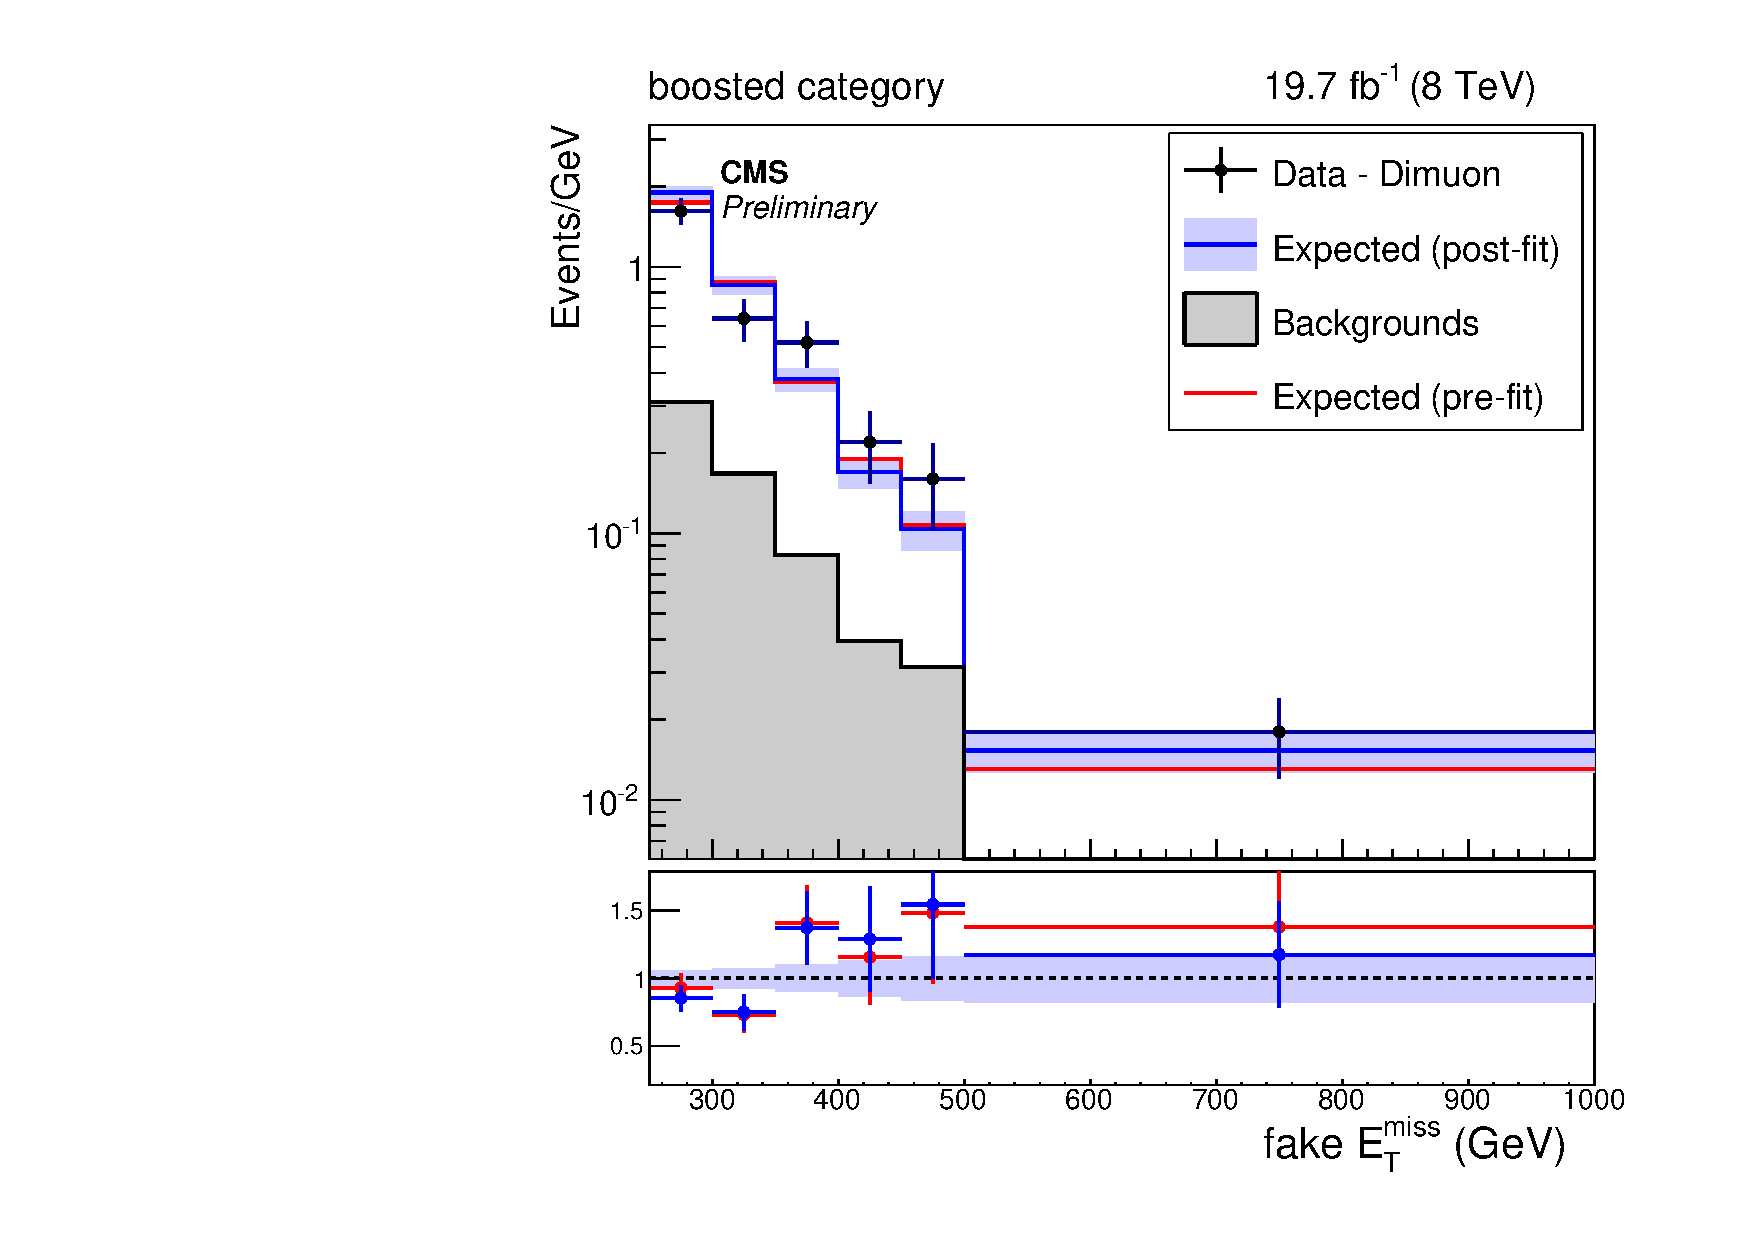
\includegraphics[width=0.32\textwidth]{fig/post_fit_zmm_boosted.pdf}
 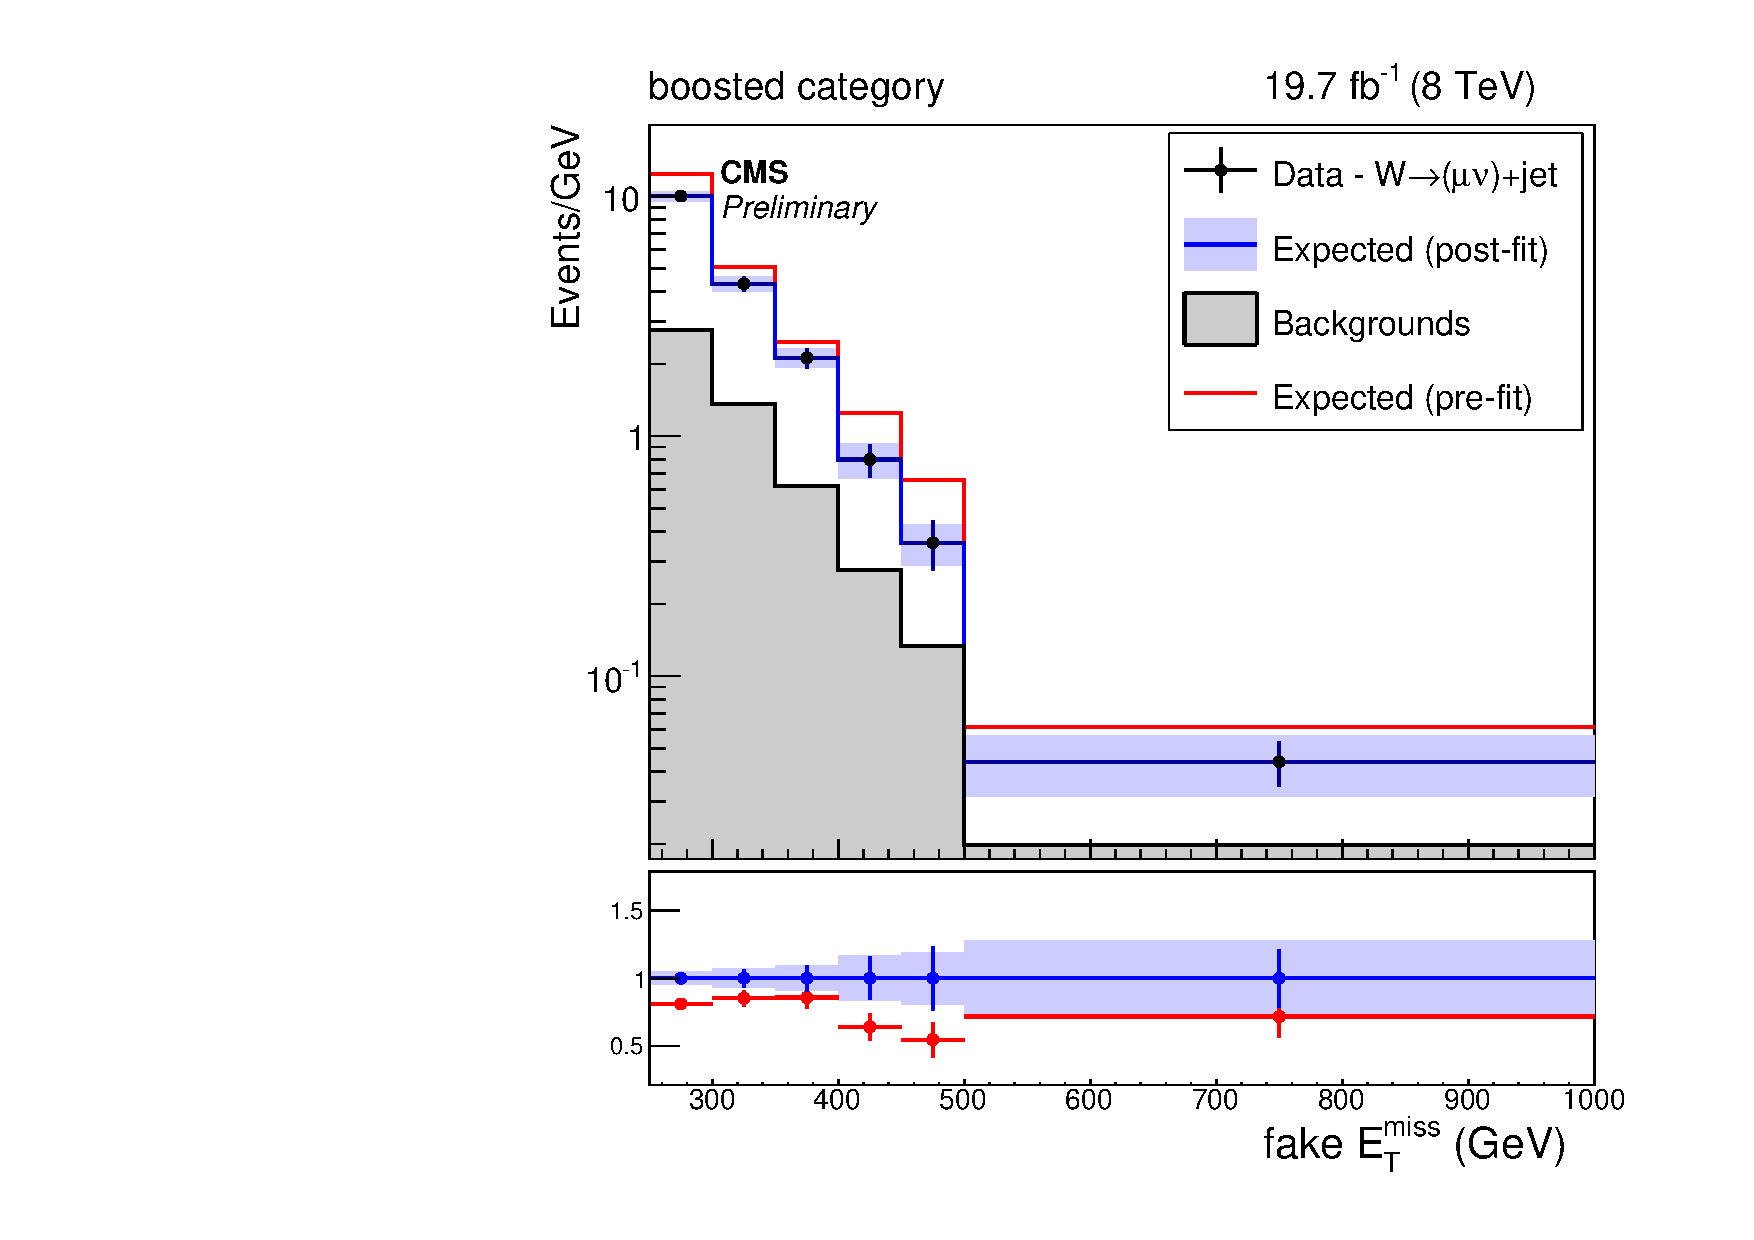
\includegraphics[width=0.32\textwidth]{fig/post_fit_wmn_boosted.pdf}\\
\end{center}
 \caption{Post-fit expected and observed (fake) \ETm distributions in the photon plus jet~(\cmsLeft), dimuon (middle) and single muon~(\cmsRight) 
 control regions from the parametric analysis. Each row, from top to bottom, shows the result of the fit in the monojet, resolved and boosted event categories 
 respectively. The red line represents the expected distribution before fitting to the control regions while the blue line shows the expectation after 
 the fit. In the the ratio, the blue and red points show the ratio of the observed data to the post-fit and pre-fit expectations 
 respectively. The blue bands indicate the statistical and systematic uncertainties from the fit.\label{fig:combined_fit_result_mbin} }
\end{figure}

\subsubsection{Single bin cut-and-count analysis}

The single bin  cut-and-count analysis has proven to be a robust style of analysis and frequently used in searches for new 
phenomena. It is however less sensitive than a shape-based analysis but may nevertheless be used as a 
cross-check of results. For the cut and count analysis, the \ETm shape is collapsed into a single bin with 
$\ETm> 500,~ 400, \textrm{and} 250$ GeV for the monojet, boosted and resolved event categories.
The threshold in the monojet category is chosen so that this analysis can also be directly compared to the DM 
interpretation results obtained in~\cite{monojet1}. For the other two categories, the threshold is relaxed due 
to the limited statistics avialable. 

The same likelihood as equation~\ref{eqn:candclh} 
is used to derive the correction for the V+jets backgrounds but with the bin index suppressed. The use of a single 
bin then removes both the power of the shape-based analysis the use of a functional form for deriving the corrections.
Table~\ref{tab:sbincandc} shows the expected yields from SM backgrounds, after applying the corrections, in 
each of the three event categories.

\begin{table*}[htbp]
  \begin{center}
    \topcaption{Expected yields for SM backgrounds and observed data for the cut-and-count analysis in the signal 
	region for each of the three event categories. The total uncertainty on the $\Zvvjets$ and $\Wlvjets$ components 
due to the statisitcal and systematic uncertainties due to the use of the three control regions is included. \emph{\textcolor{red} {Data are blind}}
      \label{tab:sbincandc}}
    \begin{tabular}{lccc}
      \hline
      \hline
      Expected Yields 		    & Boosted & Resolved & Monojet \\
      		 		    &($\ETm>$400 GeV) &($\ETm>$250 GeV) &($\ETm>$500 GeV) \\
      \hline
      \hline
      Z($\rightarrow \nu\nu$)+jets  & 117.2$\pm$9.4 (8\%)     & 445.6$\pm$20.7 (4.6\%) & 398.9$\pm$ 28.9 (7.3\%)  \\
      W($\rightarrow l\nu$)+jets    & 21.3 $\pm$3.5 (16.6\%)  & 293.9$\pm$23.0 (7.8\%) & 80.4 $\pm$ 4.9 (6.1\%) \\                
      Dibosons  		    & 23.2  & 36.5  & 7.4  \\           
      top  			    & 2.6   & 64.7  & 0.8  \\               
      Z($\rightarrow ll$)+jets      & 0.0   & 2.3   & 0.3  \\ 
      QCD		            & 0.0   & 34.2  & 0.0  \\ 
      \hline
      Total Backgrounds		    & 163.4 & 877.2 & 487.7  \\
      Data                          & X & X & X \\
      \hline
      \hline
    \end{tabular}
  \end{center}
\end{table*}


\subsubsection{Comparing the analysis}
The sensitivity of the analyses are compared by determining the expected 95\% CL upper limit on the branching ratio
of a Higgs boson with mass 125 GeV decaying invisibly. Additionally, the sensitivity is compared in the context of 
a effective field theory (EFT) by comparing the expected 90\% CL lower limit on the contact interaction scale, $\Lambda$, 
for a scalar contact interaction~\cite{Beltran:2010ww,Goodman:2010ku} as a function of the dark matter mass, $m_{DM}$. 
The limits are extracted using the combination of all three event categories. The comparison of the expected limits is 
given in Table~\ref{tab:compareanalyses}. 
 
\begin{table*}[htbp]
  \begin{center}
    \topcaption{Comparison of expected limits using the three alternate analyses.}
      \label{tab:compareanalyses}}
    \begin{tabular}{lr|ccc}
      \hline
      \hline
      	Expected limits	    & & Baseline & Parametric & Cut-and-count  \\
      \hline
       $ BR(H\rightarrow \textrm{invisibles})$, $m_{H}=125$ GeV  & &   &  & \\
       95\% CL upper limit				 & & 0.53  & 0.54 & 0.76\\
      \hline
       EFT scalar contact  $\Lambda$ (GeV) & &   &  & \\
       90\% CL lower limit			& $m_{DM}$ (GeV)&   &  & \\         
 
      & 1    				         & 448.6  & 452.3 & 424.1\\
      & 200  				 & 426.3  & 429.6 & 403.0\\
      & 400  				 & 377.8  & 380.9 & 357.7\\
      & 700  				 & 298.0  & 300.6 & 282.1\\
      & 1000 				 & 227.5  & 229.5 & 215.6\\
      
      \hline
      \hline
    \end{tabular}
  \end{center}
\end{table*}


The comparison shows that the baseline and parametric analyses perform equally well for a Higgs signal. 
This is expected due to the fact that for this signal, the monojet category is the most performing and for this category. 
In this category, the signal populates the lower end of the distribution and due to the large number of 
events in the photon control region, the systematic uncertainty (largely from the Electroweak corrections to the ratio of the differential 
cross-section between the photon and Z) dominates in this region.
The statistical component of the uncertainty, which is treated differently between the two, is therefore less relevant for the Higgs signal. 
For the EFT model, the parametric analysis performs slightly better than the baseline due to the fact that the signal for this model 
populates the higher end of the \ETm spectrum at which the parametric method is expected to constrain the V+jets backgrounds.
The cut-and-count analysis can be directly compared to the scalar EFT results obtained in ~\cite{monojet1}. This analysis shows roughly 8\% 
improvement in terms of the expected lower limit on $\Lambda$. This is due to the inclusive of the photon plus jet control region which 
significantly reduces the uncertainty on the $\Zvvjets$ background.

 

%%%%%%%%%%%%%%%%%%%%%%%%%%%%%%%%  Begin text %%%%%%%%%%%%%%%%%%%%%%%%%%%%%
%% **DO NOT REMOVE THE BIBLIOGRAPHY** which is located before the appendix.
%% You can take the text between here and the bibiliography as an example which you should replace with the actual text of your document.
%% If you include other TeX files, be sure to use "\input{filename}" rather than "\input filename".
%% The latter works for you, but our parser looks for the braces and will break when uploading the document.
%%%%%%%%%%%%%%%

%% **DO NOT REMOVE BIBLIOGRAPHY**
\bibliography{auto_generated}   % will be created by the tdr script.

%%% DO NOT ADD \end{document}!

